%%%%%%%%%%%%  Generated using docx2latex.com  %%%%%%%%%%%%%%

%%%%%%%%%%%%  v2.0.0-beta  %%%%%%%%%%%%%%

\documentclass[12pt]{article}
\usepackage{amsmath}
\usepackage{latexsym}
\usepackage{amsfonts}
\usepackage[normalem]{ulem}
\usepackage{array}
\usepackage{amssymb}
\usepackage{graphicx}
\usepackage[backend=biber,
style=numeric,
sorting=none,
isbn=false,
doi=false,
url=false,
]{biblatex}\addbibresource{bibliography.bib}

\usepackage{subfig}
\usepackage{wrapfig}
\usepackage{wasysym}
\usepackage{enumitem}
\usepackage{adjustbox}
\usepackage{ragged2e}
\usepackage[svgnames,table]{xcolor}
\usepackage{tikz}
\usepackage{longtable}
\usepackage{changepage}
\usepackage{setspace}
\usepackage{hhline}
\usepackage{multicol}
\usepackage{tabto}
\usepackage{float}
\usepackage{multirow}
\usepackage{makecell}
\usepackage{fancyhdr}
\usepackage[toc,page]{appendix}
\usepackage[hidelinks]{hyperref}
%\usepackage{hyperref}
%\hypersetup{colorlinks=false}
\usetikzlibrary{shapes.symbols,shapes.geometric,shadows,arrows.meta}
\tikzset{>={Latex[width=1.5mm,length=2mm]}}
\usepackage{flowchart}
\usepackage[paperheight=11.69in,paperwidth=8.27in,left=1in,right=1in,top=1.0in,bottom=1.0in,headheight=1in]{geometry}
\usepackage[utf8]{inputenc}
\usepackage[T1]{fontenc}
\TabPositions{0.5in,1.0in,1.5in,2.0in,2.5in,3.0in,3.5in,4.0in,4.5in,5.0in,5.5in,6.0in,}
\usepackage[margin=1cm]{caption} %  TS I added this to have the figures fit the text width


\urlstyle{same}


 %%%%%%%%%%%%  Set Depths for Sections  %%%%%%%%%%%%%%

% 1) Section
% 1.1) SubSection
% 1.1.1) SubSubSection
% 1.1.1.1) Paragraph
% 1.1.1.1.1) Subparagraph


\setcounter{tocdepth}{5}
\setcounter{secnumdepth}{5}


 %%%%%%%%%%%%  Set Depths for Nested Lists created by \begin{enumerate}  %%%%%%%%%%%%%%


\setlistdepth{9}
\renewlist{enumerate}{enumerate}{9}
		\setlist[enumerate,1]{label=\arabic*)}
		\setlist[enumerate,2]{label=\alph*)}
		\setlist[enumerate,3]{label=(\roman*)}
		\setlist[enumerate,4]{label=(\arabic*)}
		\setlist[enumerate,5]{label=(\Alph*)}
		\setlist[enumerate,6]{label=(\Roman*)}
		\setlist[enumerate,7]{label=\arabic*}
		\setlist[enumerate,8]{label=\alph*}
		\setlist[enumerate,9]{label=\roman*}

\renewlist{itemize}{itemize}{9}
		\setlist[itemize]{label=$\cdot$}
		\setlist[itemize,1]{label=\textbullet}
		\setlist[itemize,2]{label=$\circ$}
		\setlist[itemize,3]{label=$\ast$}
		\setlist[itemize,4]{label=$\dagger$}
		\setlist[itemize,5]{label=$\triangleright$}
		\setlist[itemize,6]{label=$\bigstar$}
		\setlist[itemize,7]{label=$\blacklozenge$}
		\setlist[itemize,8]{label=$\prime$}

\setlength{\topsep}{0pt}\setlength{\parindent}{0pt}

 %%%%%%%%%%%%  This sets linespacing (verticle gap between Lines) Default=1 %%%%%%%%%%%%%%


\renewcommand{\arraystretch}{1.3}

\title{ \vspace{8cm}
        Dragonereum \\
		\normalsize Digital scarcity game with blockchain and dragons}
%\date{\today}
\date{\vspace{10.5cm}
        \today \\	
		\small Version 1.1.0 Genesis}


%%%%%%%%%%%%%%%%%%%% Document code starts here %%%%%%%%%%%%%%%%%%%%



\begin{document}
\sloppy % TS this somehow prevents lines from spilling after the right margin

\maketitle
\setlength{\parskip}{9.96pt}
 \par


\vspace{\baselineskip}

\vspace{\baselineskip}

\vspace{\baselineskip}
 \par

 \par

 \par



%\abstract{
\section*{Abstract}
%\addcontentsline{toc}{section}{Abstract}
Dragonereum is a cryptocollectible game whereby users can own a dragon, trade their dragons, interbreed them and battle other dragons, collecting rewards and achievements along the way. All of these are done on the blockchain in an open, trusted and decentralized manner.\par

Our aim is to build the first truly decentralized digital scarcity game, where developers do not have any control over the game once it is deployed. The community will have the ability to verify all the transactions and actions without the involvement of trusted third parties.\par

This document discusses the technological and economic implementation of the system. It aims to describe such elements as: random number generation, decentralized breeding algorithm, battle implementation, game mechanics, and a broader economic model which emphasizes the strength of a collectible game built on blockchain.\par

In this document, we propose the philosophical background, technical foundations and the economic model of Dragonereum, whereby dragon supply is limited by the proposed game mechanics.%}

 %%%%%%%%%%%%  Starting New Page here %%%%%%%%%%%%%%

\newpage
\par


\vspace{\baselineskip}


 %%%%%%%%%%%%  This Produces Table Of Contents %%%%%%%%%%%%%%

\tableofcontents
%\addcontentsline{toc}{chapter}{Contents}

\vspace{\baselineskip}


 %%%%%%%%%%%%  Starting New Page here %%%%%%%%%%%%%%

\newpage

\vspace{\baselineskip}\section{Perspective}
%\addcontentsline{toc}{section}{State of Decentralized Games}
The appearance of decentralized games defined a new era for digital collectibles: players no longer have to rely on a trusted third party which issues assets in order to preserve the rarity of their belongings, but can fully rely on the autonomous, censorship resistant, trustless and transparent entity - the code of the smart contract.\par

However, the current offerings lack many important features of the decentralized \mbox{technology}, which limits the player’s experience to just storing assets securely on the blockchain:\par

\begin{itemize}
	\item The scope of actions one can do with his or her items is limited. Most cryptocollectible games function without a game mechanics or carefully crafted game ecosystem.\par

	\item Not properly set supply mechanisms. Unlimited supply reduces the attractiveness of a particular cryptocollectibe.\par

	\item The development teams retain full control over the released product and can add new custom-built assets at any time (though within some articulated limits) or even shut down the entire project.\par

	\item The presale monetization model is widely used thus shifting the development team’s efforts from game development to marketing and PR.\par

	\item Additionally, the current solutions still heavily rely upon a centralized infrastructure, which diminishes the advantages of blockchain usage and creates a weak spot and a single point of failure.
\end{itemize}\par

We propose a system which is built upon the basics of current technology, with advancements such as rich gamification and an in-game ecosystem with its own in-game cryptocurrency.\par

The supply of cryptocollectibles is limited by the proposed game design, and, following the game’s release, will no longer be under the team’s control. Once the game is formally released, the team will relinquish the control of token issue.\par

An improved free-to-play model is utilized where developers do not collect any fees from players for game assets and the application is built to serve with minimal ties to any servers.\par

Our long-term goal is to create a fully decentralized game, leveraging all of the unique advantages of the blockchain. More on this in \ref{Serverless application}.\par

In the following, we describe how we aim to achieve those goals. In Section \ref{Introduction to Dragonereum} we give an overview of Dragonereum’s game ecosystem. In Section \ref{Game Design Constraints} we\ describe the technological limitations faced by Dragonereum and how they are overcome, we outline how we obtain randomness and present the genetics and diversity of our dragon population.  Section \ref{Game Mechanics} explains in detail the game mechanics, and how the in-game currency is obtained and distributed. The implementation of the game is described in Section \ref{Implementation Details}, and the possible platforms with which Dragonereum can be integrated in Section \ref{Possible Integrations}. Lastly in Section \ref{Genesis} and Section \ref{GOLD} the details of the release of the genesis eggs and the Gold allocation are presented correspondingly.\par


\newpage
\vspace{\baselineskip}\section{Introduction to Dragonereum}
%\addcontentsline{toc}{section}{Introduction to Dragonereum}
  \label{Introduction to Dragonereum}  \par

Dragonereum is a cryptocollectible, person vs person game whereby users collect and breed unique dragons, engaging in battles along the way.\par

With our initial version of the decentralized application (dapp), a user will have the possibility to own and manage a dragon or a thunder of dragons. In addition to breeding and battling their dragons, users can buy and sell dragons, collect rewards, compete with other players for in-game achievements and make deals on the game’s marketplace.\par

Each dragon is owned and controlled by a particular address on the Ethereum network. Dragons are securely stored on the blockchain and cannot be modified, replicated or destroyed by any third party.\par

Every dragon has its unique set of genes which determines all features and traits of the dragon.\par

Therefore, a player will have to choose a type of dragon to control (Figure \ref{fig:A_selection_of_different_types_of_dragons__Each_row_represents_two_varieties_of_the_fire_ice_earth_air_and_cyber_type_}), decide on a battle strategy, determine which skills to train with experience earned in battles and how to get better offsprings with further improved \textit{basic skills} (\textit{attack, defense, stamina, speed, }and\textit{ intelligence}). \par



%%%%%%%%%%%%%%%%%%%% Figure/Image No: 1 starts here %%%%%%%%%%%%%%%%%%%%

\begin{Center}
\begin{figure}[!ht]
	\begin{Center}		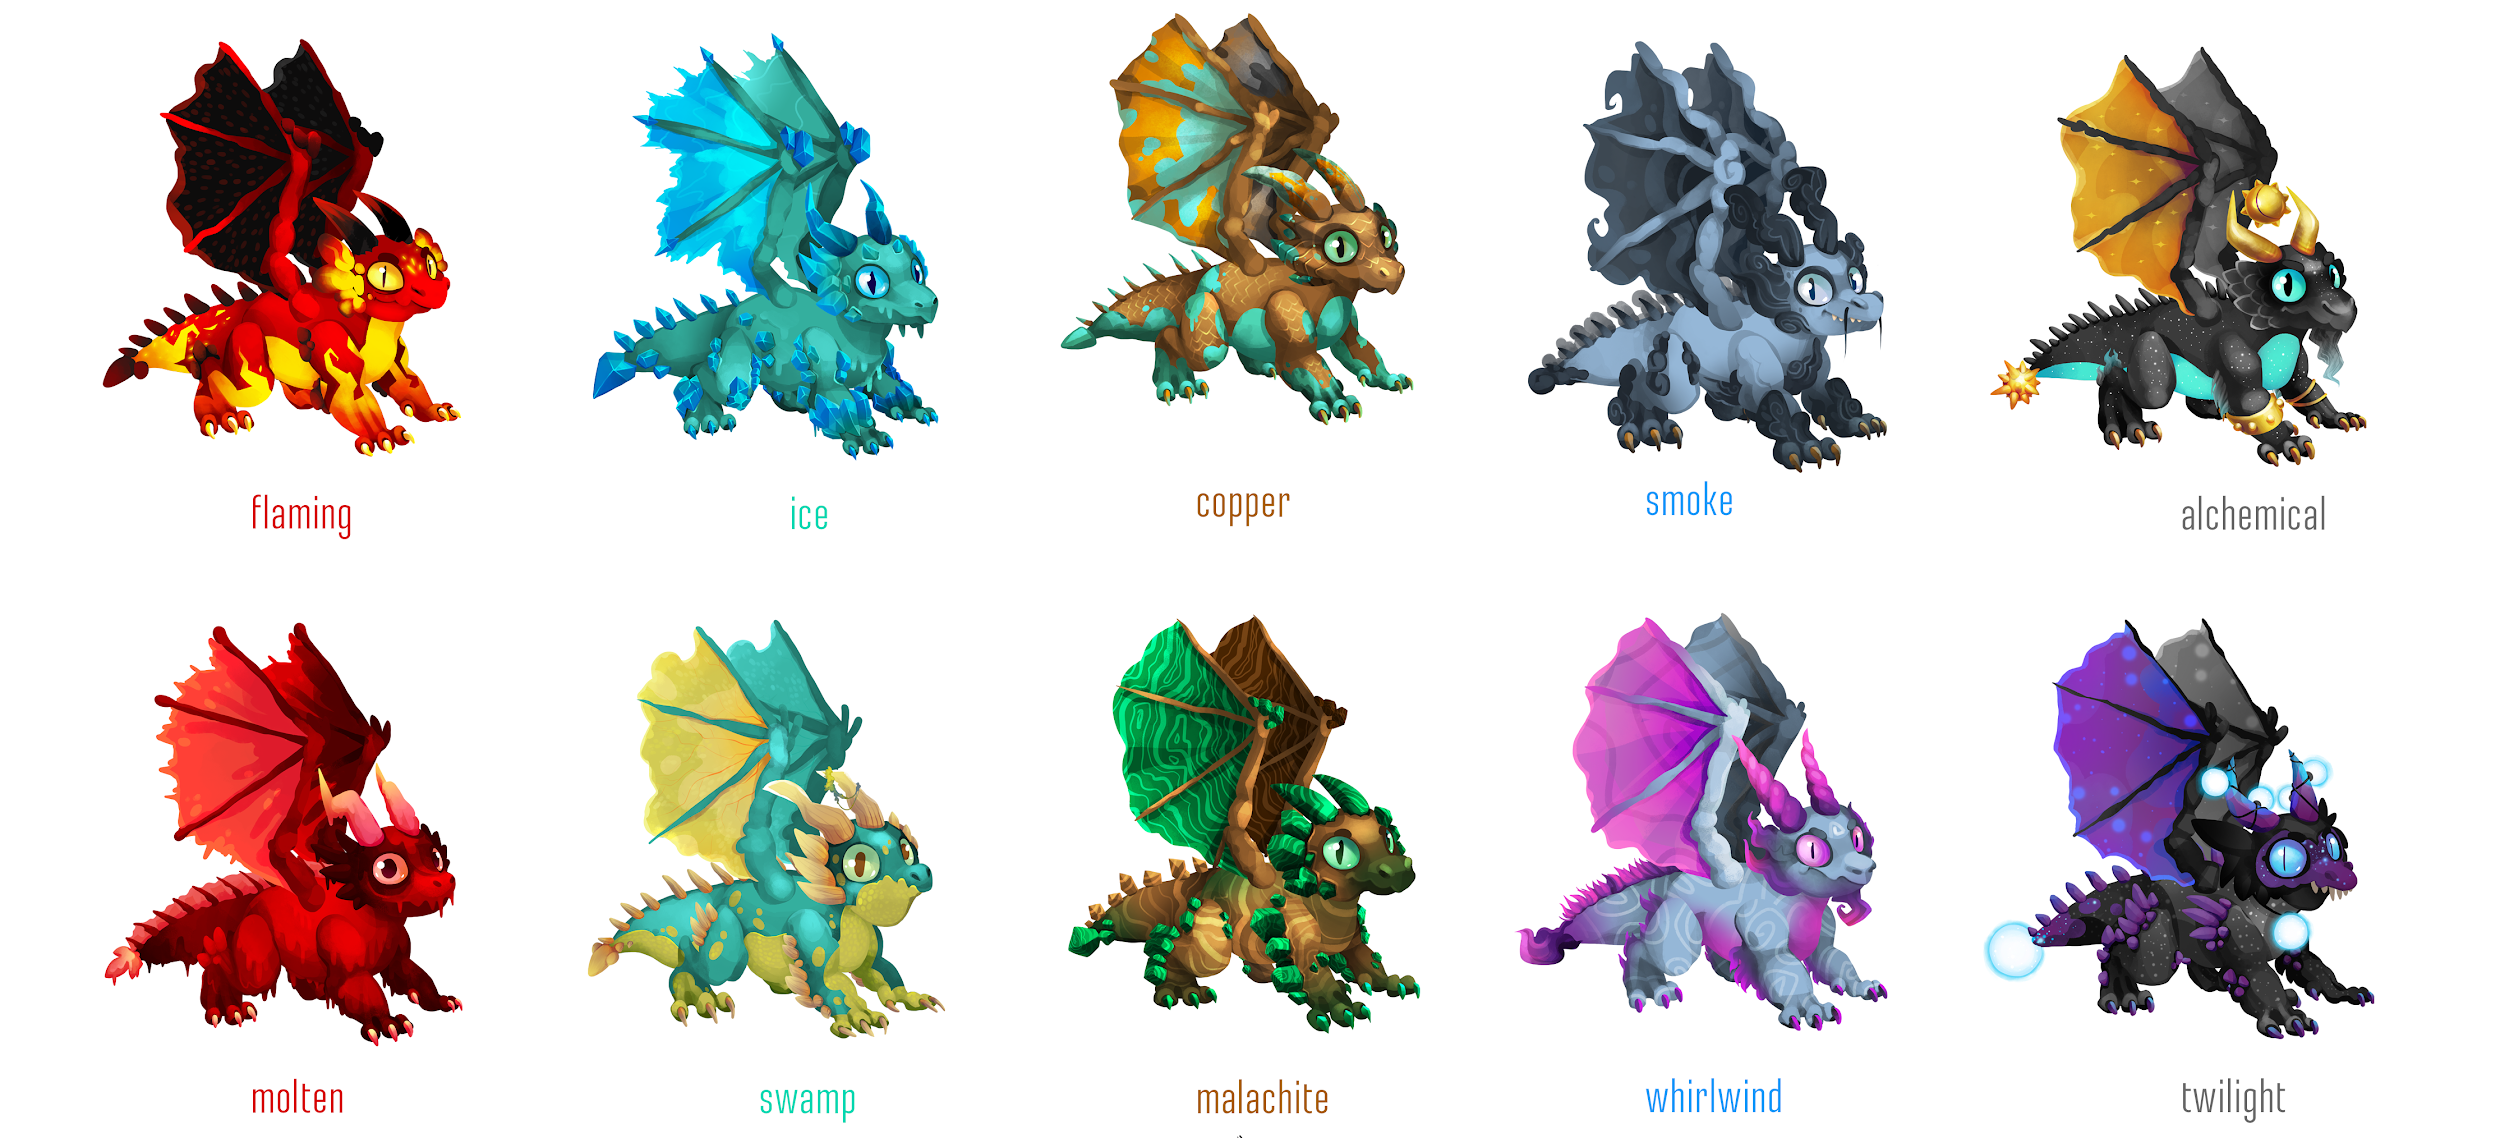
\includegraphics[width=6.27in,height=2.79in]{./media/image13.png}
		\caption{A selection of different types of dragons.  Each row represents two varieties of the fire, ice, earth, air, and cyber type. }
		\label{fig:A_selection_of_different_types_of_dragons__Each_row_represents_two_varieties_of_the_fire_ice_earth_air_and_cyber_type_}
	\end{Center}\end{figure}
\end{Center}

%%%%%%%%%%%%%%%%%%%% Figure/Image No: 1 Ends here %%%%%%%%%%%%%%%%%%%%


The player’s goal might be presented by two paths: a dragon training master or a dragon breeding master. The dragon training master will be an expert in leveling up dragons so he/she can get the strongest dragon and earn in-game rewards as a result of winning battles. The dragon breeding master will know how to interbreed dragons in order to get highly unique and valuable dragons which might be sold on the game’s marketplace. Additionally there might be some other unforeseen game paths beneficial to players which will be discovered by them.\par

The game starts with the purchase of a dragon egg or a dragon from another player or during the initial distribution of genesis eggs. In the case of an egg, a user knows the egg’s parents, but not what kind of dragon will appear from the egg, as this is decided during the egg incubation in accordance with the rules set by Dragonereum’s genetics.\par

After receiving a certain amount of experience and upgrading to the next level, a dragon will be able to either improve its skills or to breed. At that point, the user will have to decide whether to upgrade a dragon’s skillset or breed it in order to acquire a new dragon.\par

Offsprings will rarely outperform their parents right from the hatchery. However, their initial skills (at level 0) would generally be higher than the initial skills of the parent dragons. Therefore, with some training and a few level upgrades, the dragon will eventually outperform its parents.\par

As in the real world, occasionally there might be a mutation which will cause some of the traits of a new dragon to be much weaker or much stronger than those of its parents. Mutations affect individual genes, so any trait can receive a boost or a skill reset during breeding, but no one will be able to predict which gene will be affected and when.\par

As going up levels will require even more experience, it will become increasingly difficult to get any dragon’s descendants, thus limiting the total population of dragons and avoiding exponential growth.As such, the system is designed to encourage users to be active, and allow them to choose the winning strategy of their own choice.\par

There are five different dragon types (air, water, earth, fire, and cyber). Dragons of different types can interbreed, creating unique offsprings, as can be seen in Figure \ref{fig:Possible_offsprings_produced_by_dragons_of_different_types_interbreeding}.\par



%%%%%%%%%%%%%%%%%%%% Figure/Image No: 2 starts here %%%%%%%%%%%%%%%%%%%%
\begin{Center}
\begin{figure}[!ht]
	\begin{Center}		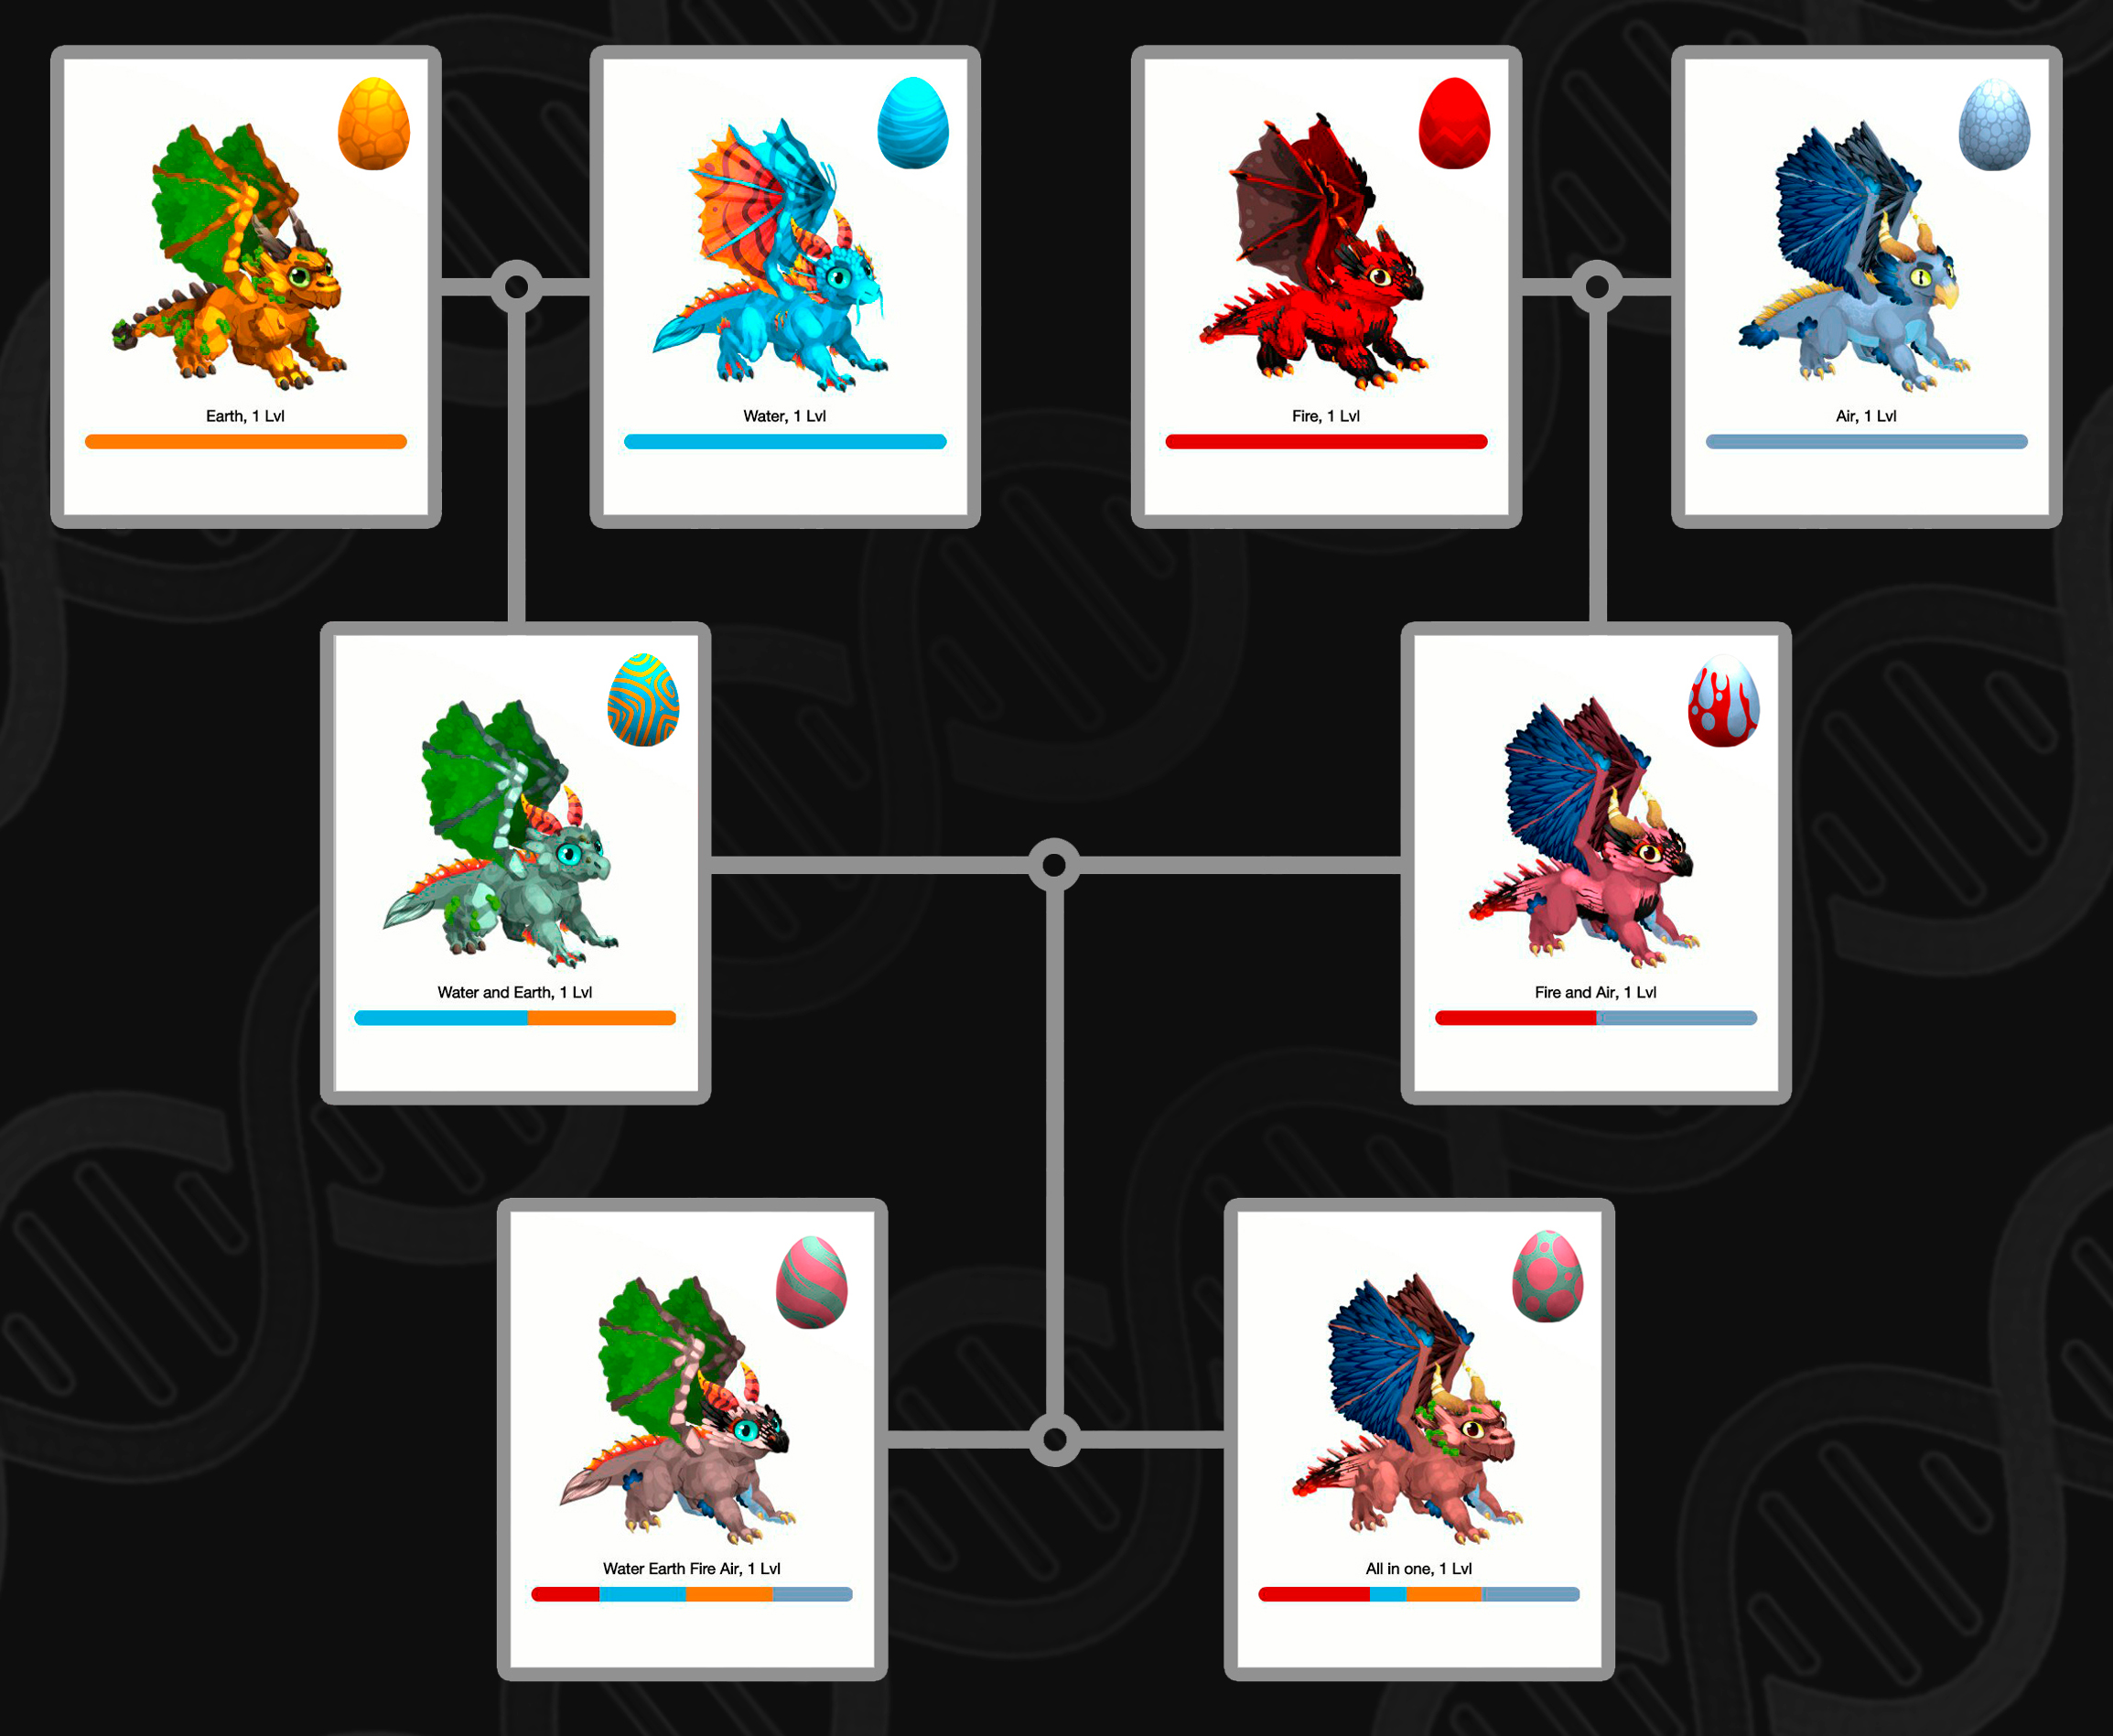
\includegraphics[width=6.27in,height=5.15in]{./media/image16.png}
		\caption{Possible offsprings produced by dragons of different types.}
		\label{fig:Possible_offsprings_produced_by_dragons_of_different_types_interbreeding}
	\end{Center}\end{figure}
\end{Center}

%%%%%%%%%%%%%%%%%%%% Figure/Image No: 2 Ends here %%%%%%%%%%%%%%%%%%%%




Every dragon has the ability to participate in battles. There will be two types of battles: regular battles and gladiator battles. Regular battles are described below, where they are referred to simply as battles, while gladiator battles will be outlined at the end of this section.\par

Taking into account the fact that battles are held on-chain they are represented not by a conjoined combat of two dragons but rather by an attack of one active dragon on another passive dragon. When a user wants their dragon to engage in a battle, providing their dragon has enough Health Points (HP), the application offers a choice of dragons of similar Dragon Strength (DS) with which it can battle. The DS is described in detail in Section \ref{Leveling up dragons}. Once a user chooses an opponent, the transaction with the battle is sent to the blockchain. As soon as the transaction is mined and included into the block, a user can see an animated battle together with the battle results\footnote{The defending dragon’s owner will similarly have the opportunity to see the animated battle once they go online}.\par

The attacking dragon always has an advantage as it can adjust its battle tactics according to its opponent’s skills. Defending dragons use the default battle tactics defined previously by the owner. All battle results are dependent on the overall skills of the battling dragons, as well as the battle tactics used during the battle. The battle tactics can be defined by two sliders:


\begin{itemize}
  \begin{samepage}
    \item The attack slider selects a value from a range between melee (short-distance attack) and ranged (long-distance attack)
    \item The action slider selects a value from a range between defense and attack
   \end{samepage}
\end{itemize}

Every move during a battle is determined by a weighted random number with the value of the weight determined by the positioning of the sliders (for example if the Action Slider is in the position of 20$\%$  defense and 80$\%$  attack - the dragon will make on average 20$\%$  defense moves and 80$\%$  attack moves). The dragons with faster speeds always make the first move.\par

\begin{samepage}
 Based on the battle tactics, settings and results of the RNG, dragons are able to:\par
 \begin{itemize}
    \item Change position
          \item Attack
          \item Stand on the defensive
          \item Use special attack or special defense
  \end{itemize}
\end{samepage}

Once the faster dragon has made the first move, the opponent has its turn. This continues until the HP for one of the dragons are depleted or the battle exceeds the move limit. If the move limit is exceeded or available gas is depleted, the dragon with higher percentage of HP compared to initial level of HP wins. If the dragons have an equal amount of HP left, the dragon which made the first move will be a winner.\par

The defeated dragon does not receive any points or bonuses. It only receives a flag protecting it from further attacks, which is valid for one day only.\par

The higher the intelligence level, the greater the chances of a dragon exploiting its \textit{special attack} or \textit{special defense} skills during the battle.\par

\textit{Special attack} or \textit{special defense} is the ability to use the special powers available for each type of dragon. It improves attack or defense during a move. These special moves use Mana.\par

The results of a battle will be displayed in a rich visual animation, which can be replayed and shared with friends.\par

A battle winner receives Experience Points (XP). When the required quantity of XP are earned, the dragon gets a level up and receives some DNA Points (DP), which can be used for breeding or converted into body part level ups and thereby improvements of skills. \par

Additionally, if the attacking dragon wins, it is credited with Gold as a bonus. Gold is an in-game cryptocurrency which will be distributed to winners from the game’s balance, and the ticker symbol for it is denoted by GOLD. The game’s creators will not have any control over Gold stored in the Dragonereum’s Treasury (which is one of the game’s smart contracts) once the control over the upgradability and halting mechanism will be transferred to the 0x000..0001 address (more details can be found in Section \ref{Serverless application}).\par

As Gold has limited availability, the reward for battle winners will decrease over time. The value of the reward will be aligned with the number of dragons in the population, Dragon Skillfulness Index (described in Section \ref{Dragon Skillfulness Index}) and the amount of Gold in the Treasury. Once the initial balance in the game's Treasury becomes depleted, the reward adjusts itself according to the sum of fees collected. These are collected for egg incubation and additional in-game features. Consequently, the first players will have an advantage with regards to Gold accumulation.\par

The only price set by Dragonereum is the amount of Gold required to incubate an egg. This way, Dragonereum controls the number of incubations along with the quantity of new dragons in its overall population.\par

Gold can also be spent on in-game services which will be offered by other players or a system. This will create a platform for social interactions between dragon owners.\par

Furthermore, as an additional incentive for players to get higher valued dragons and to engage in battles, there will be an internal ranking system, represented by a system of leaderboards, where players can keep track of their achievements and how they score against other dragon owners.\par

As already mentioned the battles described above are regular battles. Those battles allow players to earn XP and Gold from the Treasury.\par

Here, we will briefly overview gladiator battles, which are technically the same battles as regular battles, but they give players the possibility to place a bet on one of the dragons. They do not let players earn XP or Gold from the Treasury. The simplified process of the gladiator battle can be presented as follows:\par


\begin{itemize}
  \begin{samepage}
    \item A player decides to offer a dragon on the gladiator battle. He/she offers a dragon together with the amount of Eth or Gold he/she would like to place on the battle.
    \item Other players can offer their dragons for the battle together with their bets.
    \item The player who initiated the battle confirms one of the offers once the time is up for offers.
    \item Once opponents are set, other players (not necessarily those who participate in this battle) will be able to place bets.
    \item Once the timer set during the battle initiation has expired, any player can finalize the battle.
  \end{samepage}
\end{itemize}


\newpage
\vspace{\baselineskip}\section{Game Design Constraints}
%\addcontentsline{toc}{section}{Game Design Constraints}
\label{Game Design Constraints}   \par


As decentralized technologies are in their early period of development, the game was designed with several limitations in mind.\par

\textit{First of all}, the Ethereum network is currently limited to approximately 8M of gas or 15 tx/sec per block. Therefore, we had to limit the dragon population and gas-intensive events (battles, level ups, breeding, incubation, etc.) so that the game’s transactions will take just a part of the Ethereum’s bandwidth.\par

This is achieved by offering a limited quantity of genesis eggs and constraining the breeding speed which will limit the supply of new dragons and thus keep the overall game bandwidth within the Ethereum’s network capacity.\par

These initial limitations set a foundation for a broader game economy: supply of in-game currency, cost of incubation, size of a battle reward.\par

\textit{Secondly}, as every interaction with smart contracts requires a payment of a miners fee we have to limit the associated mental costs by reducing the number of actions that players have to make and make the code as efficient as possible.\par

\textit{Thirdly}, as Ethereum blocks are mined every 15 seconds we have to limit the interactivity of the game mechanics to suit this model.\par

Additionally, we want to mention that the proposed random number generator (RNG) is in reality a pseudorandom number generator (PRNG) and true randomness is currently unachievable on the blockchain. Therefore, for high value transactions we offer a solution which minimizes the chances of exploiting the game’s algorithms.\par

 %%%%%%%%%%%%  Starting New Page here %%%%%%%%%%%%%%

\newpage
\vspace{\baselineskip}\section{Obtaining Randomness}
%\addcontentsline{toc}{section}{Obtaining Randomness}
\label{Obtaining Randomness}   \par

There are two main approaches used for random number generation. The first relies on some physical phenomenon which is expected to be random. The second relies on a computational algorithm. The latter uses some initial value to generate a random number. However, a generated random number can be reproduced if the initial value (or source of it) and the RNG algorithm is known to the attacker. Hence, this approach, known as pseudorandom, is not truly random.\par

For some industries (e.g. online gambling), obtaining randomness, or to be more precise pseudorandomness, is a complex issue as the random numbers which influence a game’s outcome should be equally unpredictable for all parties.\par

Within the current online apps, there are multiple ways to obtain randomness, either independently or by relying on third parties. However, users of such apps rarely have the possibility to validate the process of obtaining these random numbers.\par

On the other hand, for decentralized apps (dapps), where an outcome relies upon the random number, this issue becomes increasingly important due to the limited availability of RNG methods, the price associated with the the use of current solutions and the time required for RNG.\par

To build a proper decentralized game, where an outcome is defined by a random number, the following specifications of RNG must be met  \cite{Tomas_Draksas_2017_Aug_28}:\par

\begin{enumerate}
	\item The RNG can generate a random number in a short period of time, ideally in less than 1 second.\par

	\item The RNG can be trusted and verified by being stored on a blockchain.\par

	\item The RNG should be capable of serving a large number of players simultaneously.\par

	\item A low gas/transaction cost to obtain a random number.
\end{enumerate}\par

Below we describe several different approaches to obtaining random numbers for Ethereum dapps available today.\par

\vspace{\baselineskip}
\subsection{Data from blockchain blocks}
%\addcontentsline{toc}{subsection}{Data from blockchain blocks}
\label{Data from blockchain blocks}  \par

It is possible to obtain a random (pseudo-random) number from the block data directly, i.e. based on a block number, a block hash, etc. This approach is fast (the random number is generated in the next mined block) and relatively cheap, but there is a possibility that the miners can influence the output of the block in order to affect a generated number. More on this further down.\par


\vspace{\baselineskip}
\subsection{Use of oracles}
%\addcontentsline{toc}{subsection}{Use of oracles}
\label{Use of oracles}  \par

This approach is based on some trusted external source of randomness, e.g. www.random.org, which is then delivered to the blockchain by other trusted external sources, e.g. http://www.oraclize.it  \cite{Oraclize_2017_May_18}.\par

This implementation is simple, but its weak spot is that oracles could also be compromised  \cite{Dao_Casino_Ksenya_Serova_2017_Jun_27}. It also takes longer to obtain a random number as two blockchain transactions are needed. In our tests, it took around 30 seconds to get a random value using this approach.\par

\vspace{\baselineskip}
\subsection{Commit-reveal}
%\addcontentsline{toc}{subsection}{Commit-reveal}
\label{Commit-reveal}  \par

RNG by this method requires two steps. During the first step, participants send hashes of random values and deposit a pledge. During the second step, the sent values are disclosed and a random number is generated based on these initial values  \cite{Dao_Casino_Ksenya_Serova_2017_Jun_27}. The pledge is required to ensure the faithfulness of the participants. This method is used by RanDAO, Sleth, and Maker-Darts  \cite{Dao_Casino_Ksenya_Serova_2017_Jun_27}.\par

The disadvantages of this method are that a fee is required for most implementations in order to involve participants for random number generation, and that this method is subject to DDOS attacks. The latter results in a loss of pledges by honest participants  \cite{Dao_Casino_Ksenya_Serova_2017_Jun_27}.\par


\vspace{\baselineskip}
\subsection{Future blocks}
%\addcontentsline{toc}{subsection}{Future blocks}
\label{Future blocks}  \par

During this RNG, a user sends a transaction that calls the RNG function. The sender's address is added to a list of requests by the RNG smart contract. In the next step, a user requests a random number via another transaction after some blocks have been mined by the network. The required action is taken using a generated random number, based on an initial input and some hashing algorithm, e.g. sha256.\par

This approach is slower than the other solutions (2 blocks will take about 30 seconds) and the current limitations of the EVM (Ethereum Virtual Machine) allow us to look back only 256 blocks. Hence, a user could just skip a generated number if it does not match his/her expectations.\par

\vspace{\baselineskip}
\subsection{Signidice algorithm}
%\addcontentsline{toc}{subsection}{Signidice algorithm}
\label{Signidice algorithm}  \par

This approach of RNG is described in Gluk256 repository  \cite{Dao_Casino_Ksenya_Serova_2017_Jun_27},  \cite{Gluk256_2016_Aug_26}. The Ethereum smart contract receives a newly generated public key from the owner and awaits a value from the user. After receipt of this value, the owner hashes it with a private key, thus generating a required random number, which might be confirmed by an already published public key.\par

Regardless of the fact that a penalty for parties which do not reveal their signatures should be implemented, it is still possible to use this method for our use-cases. However, we consider this approach to be too complex for our initial requirements (more on this below).\par

\vspace{\baselineskip}
\subsection{Dragonereum’s solution}
%\addcontentsline{toc}{subsection}{Dragonereum’s solution}
\label{Dragonereums solution}  \par

According to the initial requirements, the RNG has to generate a random number as fast as possible (ideally it should take less than 1 second, however, the processing time is currently limited by Ethereum’s rate of block creation). The best solution in this case is to use data from a blockchain block.\par

Our solution uses a block’s hash to generate random numbers. As every transaction rely on different input data (dragon genetics, battle skills and tactics, etc), different dragons will receive different results even if several transactions are included in one block and therefore have same random number,\par

\begin{Center}
\textit{uint256(keccak256(abi.encodePacked(blockhash(block.number - 1), now)));}
\end{Center}\par

where \textit{ now} is the block.timestamp.\par

For complex computations where several different random numbers are required we use the remainder of the division of the initially generated random number and repeat the procedure until the necessary amount of random numbers is obtained.\par

\vspace{\baselineskip}
\subsection{Miner attack resistance analysis}
%\addcontentsline{toc}{subsection}{Miner attack resistance analysis}
\label{Miner attack resistance analysis}  \par

The aforementioned algorithm is subject to miner attacks as the timestamp can be manipulated by a miner and several transactions can be included in the block in order to receive the \textit{\_seed }which matches the desired value.\par

The timestamp submitted by a miner has to comply with the following rules:\par

\begin{itemize}
	\item The timestamp of the current block has to be greater than the timestamp of the parent block\par

	\item The timestamp can not be set too far into the future\par

	\item The timestamp should not be earlier than when the block was actually mined in order to keep the difficulty as low as possible.
\end{itemize}\par

Larger miners can safely manipulate the timestamp for some time without negative consequences. Therefore, we assume that a timestamp can be manipulated by a miner in the range of approximately 10 seconds (the timestamp in the Ethereum blockchain stored in a second format), as constant higher deviation of the timestamp will result in a rejection of the block by other nodes. \par

Therefore, a malicious miner can have 10 times higher possibilities to manipulate the random number generation outcome. However, the use of the pure implementation of this RNG algorithm is limited in Dragonereum just by the battle transactions.\par

\begin{justify}
\textbf{Low-value transactions}
\end{justify}\par

\begin{justify}
Battle transactions (regular battles only) allow players to earn Gold and XP for dragons participating in battles. We assume that these kind of transactions are low-value as each battle rewards users with a limited amount of in-game cryptocurrency and XP which does not have direct monetary value.
\end{justify}\par

\begin{justify}
Battle transactions can not be compromised by regular players as the RNG includes block.timestamp which is set by a miner. Players can guess what the timestamp will be by looking into historical data and making some assumptions, however it will still be random as it can not be determined in advance with certainty.
\end{justify}\par

\begin{justify}
However, this approach is easily exploitable by a sophisticated attacker who can employ a smart contract to check the value of block.timestamp during the block creation. We overcome this issue by allowing this function to be called only by an externally owned accounts  \cite{account_types_gas_and_transactions} (onlyHuman modifier).
\end{justify}\par

\begin{justify}
Miners on the other hand will have the possibility to alter the timestamp in order to benefit their own battle transactions. However, their possibilities for manipulation are limited by the factors outlined above. Additionally, to gain advantage by manipulating a timestamp the miner will have to do it over a long period of time, which will have a high chance of being noticed by the community. Thus, hurting the goodwill of the company behind it and potentially costing much more in lost profits since part of the miners might potentially leave the mining pool.
\end{justify}\par

\begin{justify}
Additionally, regular players will be able to win the same amount of Gold (a maximum of 200 GOLD at the initial stage of the game, given the player has a dragon of DS close to the maximum) just by battling dragons of similar DS.
\end{justify}\par

\begin{justify}
Also, recent developments evidentiated that miners do not easily tend towards manipulation techniques even when a much higher value is at stake  \cite{SECBIT_2018_Aug_22}. Therefore, we assume that the proposed RNG is sufficient for these use cases.
\end{justify}\par

\textbf{High-value transactions}\par

There are two types of transactions that we consider to be high-value. Those are:\par

\begin{itemize}
	\item Breeding transactions\par

	\item Gladiator battle transactions
\end{itemize}\par

\begin{justify}
In the case of high-value transactions an attacker will have a much greater economic motivation to engage in a possible transaction manipulation. For both of these types of transactions we offer certain tweaks to the original algorithm in order to make it more manipulation resistant.
\end{justify}\par

\begin{justify}
With an original algorithm an attacking miner has a very high chance to clone the required genes (in an ideal situation it is 7/16 or 43.75$\%$  for an individual gene and 0.09$\%$  ( $10*(7/16*9/10)^{10}$) for the whole genome, please refer to Section  \ref{Blockchain breeding algorithm}). In order to prevent this, we supplemented our RNG algorithm with additional steps in the case of a breeding transaction.
\end{justify}\par

\begin{justify}
Instead of $``$direct$"$ breeding, in which case a miner will have an unlimited number of chances to initiate a breeding during a suitable moment, we introduce a Nest - an incubator with two eggs waiting to be hatched. Only one egg can be send to the Nest in a block and each forthcoming egg (i) opens the earliest placed egg in the Nest (i-2).
\end{justify}\par

\begin{justify}
A regular player will have the same likelihood of predicting the timestamp that a miner sets for a block, however, now the miner only has a limited amount of time to find a suitable moment to implement the attack, as other miners might include the transaction of someone else sending an egg to the Nest, thus hatching the egg of the attacker.
\end{justify}\par

In\ the case of gladiator battles - the feature which potentially might store the highest amount of value for the widest array of stakeholders, we offer a variation of the Future blocks approach (see Section  \ref{Future blocks}). When a gladiator battle is set and an initial timer has run out any player can run the battle at any moment. In the case when the 256 block limit is exceeded, a new timer is set in the future and once it runs out, anyone can start the battle at any time.\par

This approach allows any interested party to conduct a battle, therefore withdrawing the possibility of waiting for an appropriate moment by those players who will not be happy with the outcome.\par


\vspace{\baselineskip}
The proposed solutions are not ideal and have a degree of vulnerability, however at the current state of decentralized technology and given the use cases, those solutions offer a balance between the simplicity of implementation/usability and the resistance to an attack.\par

We hope that with the introduction of true randomness in a future development of the Ethereum ecosystem there will be a possibility to switch to more secure algorithms which at the same time will not be more difficult from the player’s point of view.\par

\newpage
\vspace{\baselineskip}\section{Blockchain Genetics}
%\addcontentsline{toc}{section}{Blockchain Genetics}
\label{Blockchain Genetics}   \par

\subsection{Blockchain breeding algorithm}
%\addcontentsline{toc}{subsection}{Blockchain breeding algorithm}
  \label{Blockchain breeding algorithm}  \par

A major limitation of current non-blockchain games is the process of new character creation. Current solutions allow the user to choose some characteristics of a character or supply a default character with a preconfigured range of abilities. Additionally, all current solutions are centralized by design, so the player does not control or have the ability to verify the process of game character creation, the number of created characters or their set of skills.\par

As such, the game’s creators can, at any moment, release newly created characters with an improved skill set or unique appearance, thus destroying all economic incentives of current players who invested time and money into their characters. This is particularly important for cases where all created characters are collectibles.\par

We propose a system whereby any third party (even the creators) has no control over new character creation after the release of the system.\par

To build such a system, all steps of the creation process should be done on blockchain. In order to do that, two main principles must be met:\par

\begin{enumerate}
	\item A random number has to be generated on the blockchain or at least stored on the blockchain.\par

	\item Character breeding also has to be done on the blockchain via a publicly accessible smart contract.
\end{enumerate}\par

RNG was already described in this document and here we will dig into on-chain breeding in the context of its implementation on the EVM.\par

In Dragonereum, dragon genetics play a crucial role as they determine every aspect of a dragon’s character, appearance and fighting abilities. Thus they define the market value of a particular dragon as a cryptocollectible item. As such we attempted to make the genetics of dragons similar to the genetics of real-world animals, nevertheless adding some additional features as we are talking about dragons, aren’t we? Additionally, we have to keep the complexity at a level appropriate to EVM.\par

Also in order to minimize costs, we reduced the complexity of the smart contract to the level where users pay less, but the predictability of breeding is not sacrificed.\par

We hope that with future releases of new solutions and Ethereum protocols, the cost of breeding will be reduced and there will be a possibility to switch to more advanced forms of breeding algorithms.\par

In the following text we will describe the breeding algorithm.\par

Two dragons upgraded to a certain level can breed and produce an egg. This egg can be incubated\footnote{The egg is placed in the Nest. Once the third egg is placed to the Nest, the first egg placed there will hatch, so the addition of the third egg in the incubator opens the first egg. The process of hatching continues with the addition of every new egg, out of the eggs inside the Nest, the egg that was in there first hatches everytime a new egg is added.}  and a new dragon with the traits of both parents will be born.\par

As can be seen from Dragonereum’s egg code (part of a ERC721 token) it stores just the information about parents so the traits of a dragon are determined from this information during the incubation.\par



\begin{footnotesize}
\begin{verbatim}
struct Egg {
       uint256[2] parents;
       uint8 type; // type of a dragon (only for genesis eggs)
   }

\end{verbatim}
\end{footnotesize}

A hatched dragon on the other hand has much more information stored inside its ERC721 code.\par

\begin{footnotesize}
\begin{verbatim}
// health and mana are multiplied by 100
struct HealthAndMana {
       uint256 timestamp; // timestamp of last HP or mana update
       uint32 remainingHealth; // remaining from last update
       uint32 remainingMana; // remaining from last update
       uint32 maxHealth;
       uint32 maxMana;
}
struct Level {
       uint8 level; // current level of dragon
       uint8 experience; // XP current level
       uint16 points; // DNA points
}
struct Tactics {
       uint8 melee; // ranged/melee tactics in percentages
       uint8 attack; // defense/attack tactics in percentages
}
struct Battles {
       uint16 wins;
       uint16 defeats;
}
// multilpied by 100
struct Skills {
       uint32 attack;
       uint32 defense;
       uint32 stamina;
       uint32 speed;
       uint32 intelligence;
}
// types:
// 0 - water, 1 - fire, 2 - air, 3 - earth, 4 - cyber
struct Dragon {
       uint16 generation;
       uint256[4] genome;
       uint256[2] parents;
       uint8[11] types; // array of weights of dragon's types
       uint256 birth; // timestamp
}
Dragon[] public dragons;
// dragon id -> value
mapping (uint256 => bytes32) public names;
mapping (uint256 => HealthAndMana) public healthAndMana;
mapping (uint256 => Tactics) public tactics;
mapping (uint256 => Battles) public battles;
mapping (uint256 => Skills) public skills;
mapping (uint256 => Level) public levels;
mapping (uint256 => uint32) public coolness; // Dragon Skillfulness Index multiplied by 100
// id -> type of skill (dragon type)
mapping (uint256 => uint8) public specialAttacks;
mapping (uint256 => uint8) public specialDefenses;
// classes:
// 0 - no skill
// 1 - attack multiplier
// 2 - defense multiplier
// 3 - stamina multiplier
// 4 - speed multiplier
// 5 - intelligence multiplier
// 6 - healing
// 7 - mana regeneration
// id -> class
mapping (uint256 => uint8) public peacefulSkills;
// classes:
// 1 - attack, 2 - defense, 3 - stamina, 4 - speed, 5 - intelligence
// id -> class -> effect
mapping (uint256 => mapping (uint8 => uint32)) public buffs;

\end{verbatim}
\end{footnotesize}

The genome is stored in an array of 4 numbers of uint256 type, that equals to 128 bytes in total. As it is shown below this is a sufficient size from the diversity perspective.\par

Dragonereum’s dragons have 10 body parts, each consisting of 4 sets of genes, therefore, an example of the whole genome of a dragon will look as follows:\par

\textbf{0302841} 0400941 0204180 0207320 0105800 \textbf{0102291} 0407630 0401391 \textbf{0201591} 0306510 0300351 0202210 \textbf{0005190} 0305350 0007531 0204551 \textbf{0305021} 0004421 0005011 0409360 \textbf{0202431} 0107660 0006810 0103420 0202250 \textbf{0002831} 0103821 0304430 \textbf{0407111} 0107070 0004201 0102570 \textbf{0405551} 0303861 0104861 0306670 0200110 \textbf{0105031} 0104531 0106750\par

The order of the body parts is: head, eyes, horns, body, wings, arms, legs, tail, spikes, and skin. The active gene describing the body part in each set of 4 is written in bold type. Each particular body part gives the dragons a boost for a set of\textit{ basic skills}.\ For example, the head is responsible for attack, stamina, and intelligence, while the eyes are responsible for defense, speed and intelligence (see Section \ref{Body parts and basic skills}).\par

The genome sequence determines the appearance and skills of a dragon. Also individual genes from it take part in the breeding process. In this example the first body part is represented by the following code:\par

\textbf{0302841} 0400941 0204180 0207320\par


\vspace{\baselineskip}

\begin{samepage}
Let's break down the first gene, which is the dominant one in this case, of the first set of genes and see how it influences the appearance of our theoretical dragon: 

03 - dragon type (earth dragon) \\
02 - gene variety (copper dragon) \\
84 - gene level \\
1 - dominant 
\end{samepage}

Similar to the natural world, every gene can be recessive (weak) or dominant (strong) and has an influence on the outcome of genome creation during breeding. Every new dragon has two sets of genes (one from each parent) according to the following rules:
\begin{itemize}
	\item The dominant gene always suppresses the recessive gene.
	\item A pair of recessive genes will always be transferred to the next generation.
\end{itemize}

An active gene determines the appearance and skills of a dragon. Active genes are defined by another set of rules:

\begin{enumerate}
	\item If a pair of genes consists of two dominant genes, the first dominant gene will become the active gene for this dragon.
	\item If a pair of genes consists of a dominant and a recessive gene, the dominant gene will become the active gene.
	\item If a pair of genes consists of two recessive genes, then the first of the pair will become the active gene.
\end{enumerate}

Therefore, according to rule 1, 0302841 from the example above, is our active gene which determines the appearance of the head as both genes in the first pair are dominant. As can be seen from Figure \ref{fig:A_dragon_with_an_Earth_Copper_head_whose_genome_is_studied_in_the_text} this dragon will have a Copper dragon's head.\par

\begin{Center}
%%%%%%%%%%%%%%%%%%%% Figure/Image No: 3 starts here %%%%%%%%%%%%%%%%%%%%

\begin{figure}[H]
	\begin{Center}
		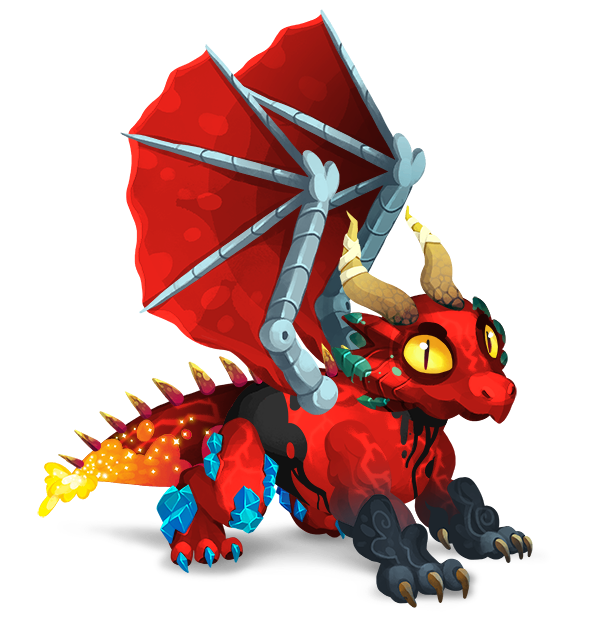
\includegraphics[width=4.26in,height=4.38in]{./media/BGimage28.png}
		\caption{A dragon with an Earth Copper head, whose genome is studied in the text.}
		\label{fig:A_dragon_with_an_Earth_Copper_head_whose_genome_is_studied_in_the_text}
	\end{Center}
\end{figure}


%%%%%%%%%%%%%%%%%%%% Figure/Image No: 3 Ends here %%%%%%%%%%%%%%%%%%%%
\end{Center}\par

Dragonereum’s breeding algorithm is represented below.\par

\begin{footnotesize}
\begin{verbatim}
function breeding(
       uint8[16][10] memory _momGenome, // parsed genome
       uint8[16][10] memory _dadGenome, // parsed genome
       uint8 _uglinessChance // if inbreeding
   ) internal returns (uint8[16][10] genome) {
       uint256 _seed = random.random(2**256 - 1);
       uint256 _random;
       uint8 _mutationChance = _uglinessChance == 0 ? MUTATION_CHANCE :
_uglinessChance;
       uint8 _geneType;
       for (uint8 i = 0; i < 10; i++) {
           (_random, _seed) = _getSpecialRandom(_seed, 4); // 0..9999
           genome[i] = _calculateGen(_momGenome[i], _dadGenome[i], (_random % 
16).toUint8()); // get 1 random pair from 16 genes pairs
           (_random, _seed) = _getSpecialRandom(_seed, 1); // 0..9
           if (_random < _mutationChance) {
               _geneType = 0;
               if (_uglinessChance == 0) {
                   (_random, _seed) = _getSpecialRandom(_seed, 2); // 0..99
                   _geneType = (_random % 9).add(1).toUint8(); // 1..9
               }
               genome[i] = _mutateGene(genome[i], _geneType);
           }
       }
   }
\end{verbatim}
\end{footnotesize}

An example of a breeding can be found in our article explaining breeding, mutations and inbreeding effects on dragons \cite{Dragonereum_2018_Mar_26}.\par 

This approach allows us to create a truly trusted world of cryptocollectible dragons, where everyone will be able to observe the breeding process, and no one will be able to influence the results, thus completely removing the necessity of trust as is the case with other solutions available today.

\vspace{\baselineskip}\subsection{Dragon diversity }
%\addcontentsline{toc}{subsection}{Dragon diversity }
\label{Dragon diversity}   


\begin{Center}
%%%%%%%%%%%%%%%%%%%% Figure/Image No: 3 starts here %%%%%%%%%%%%%%%%%%%%

\begin{figure}[!ht]
	\begin{Center}
		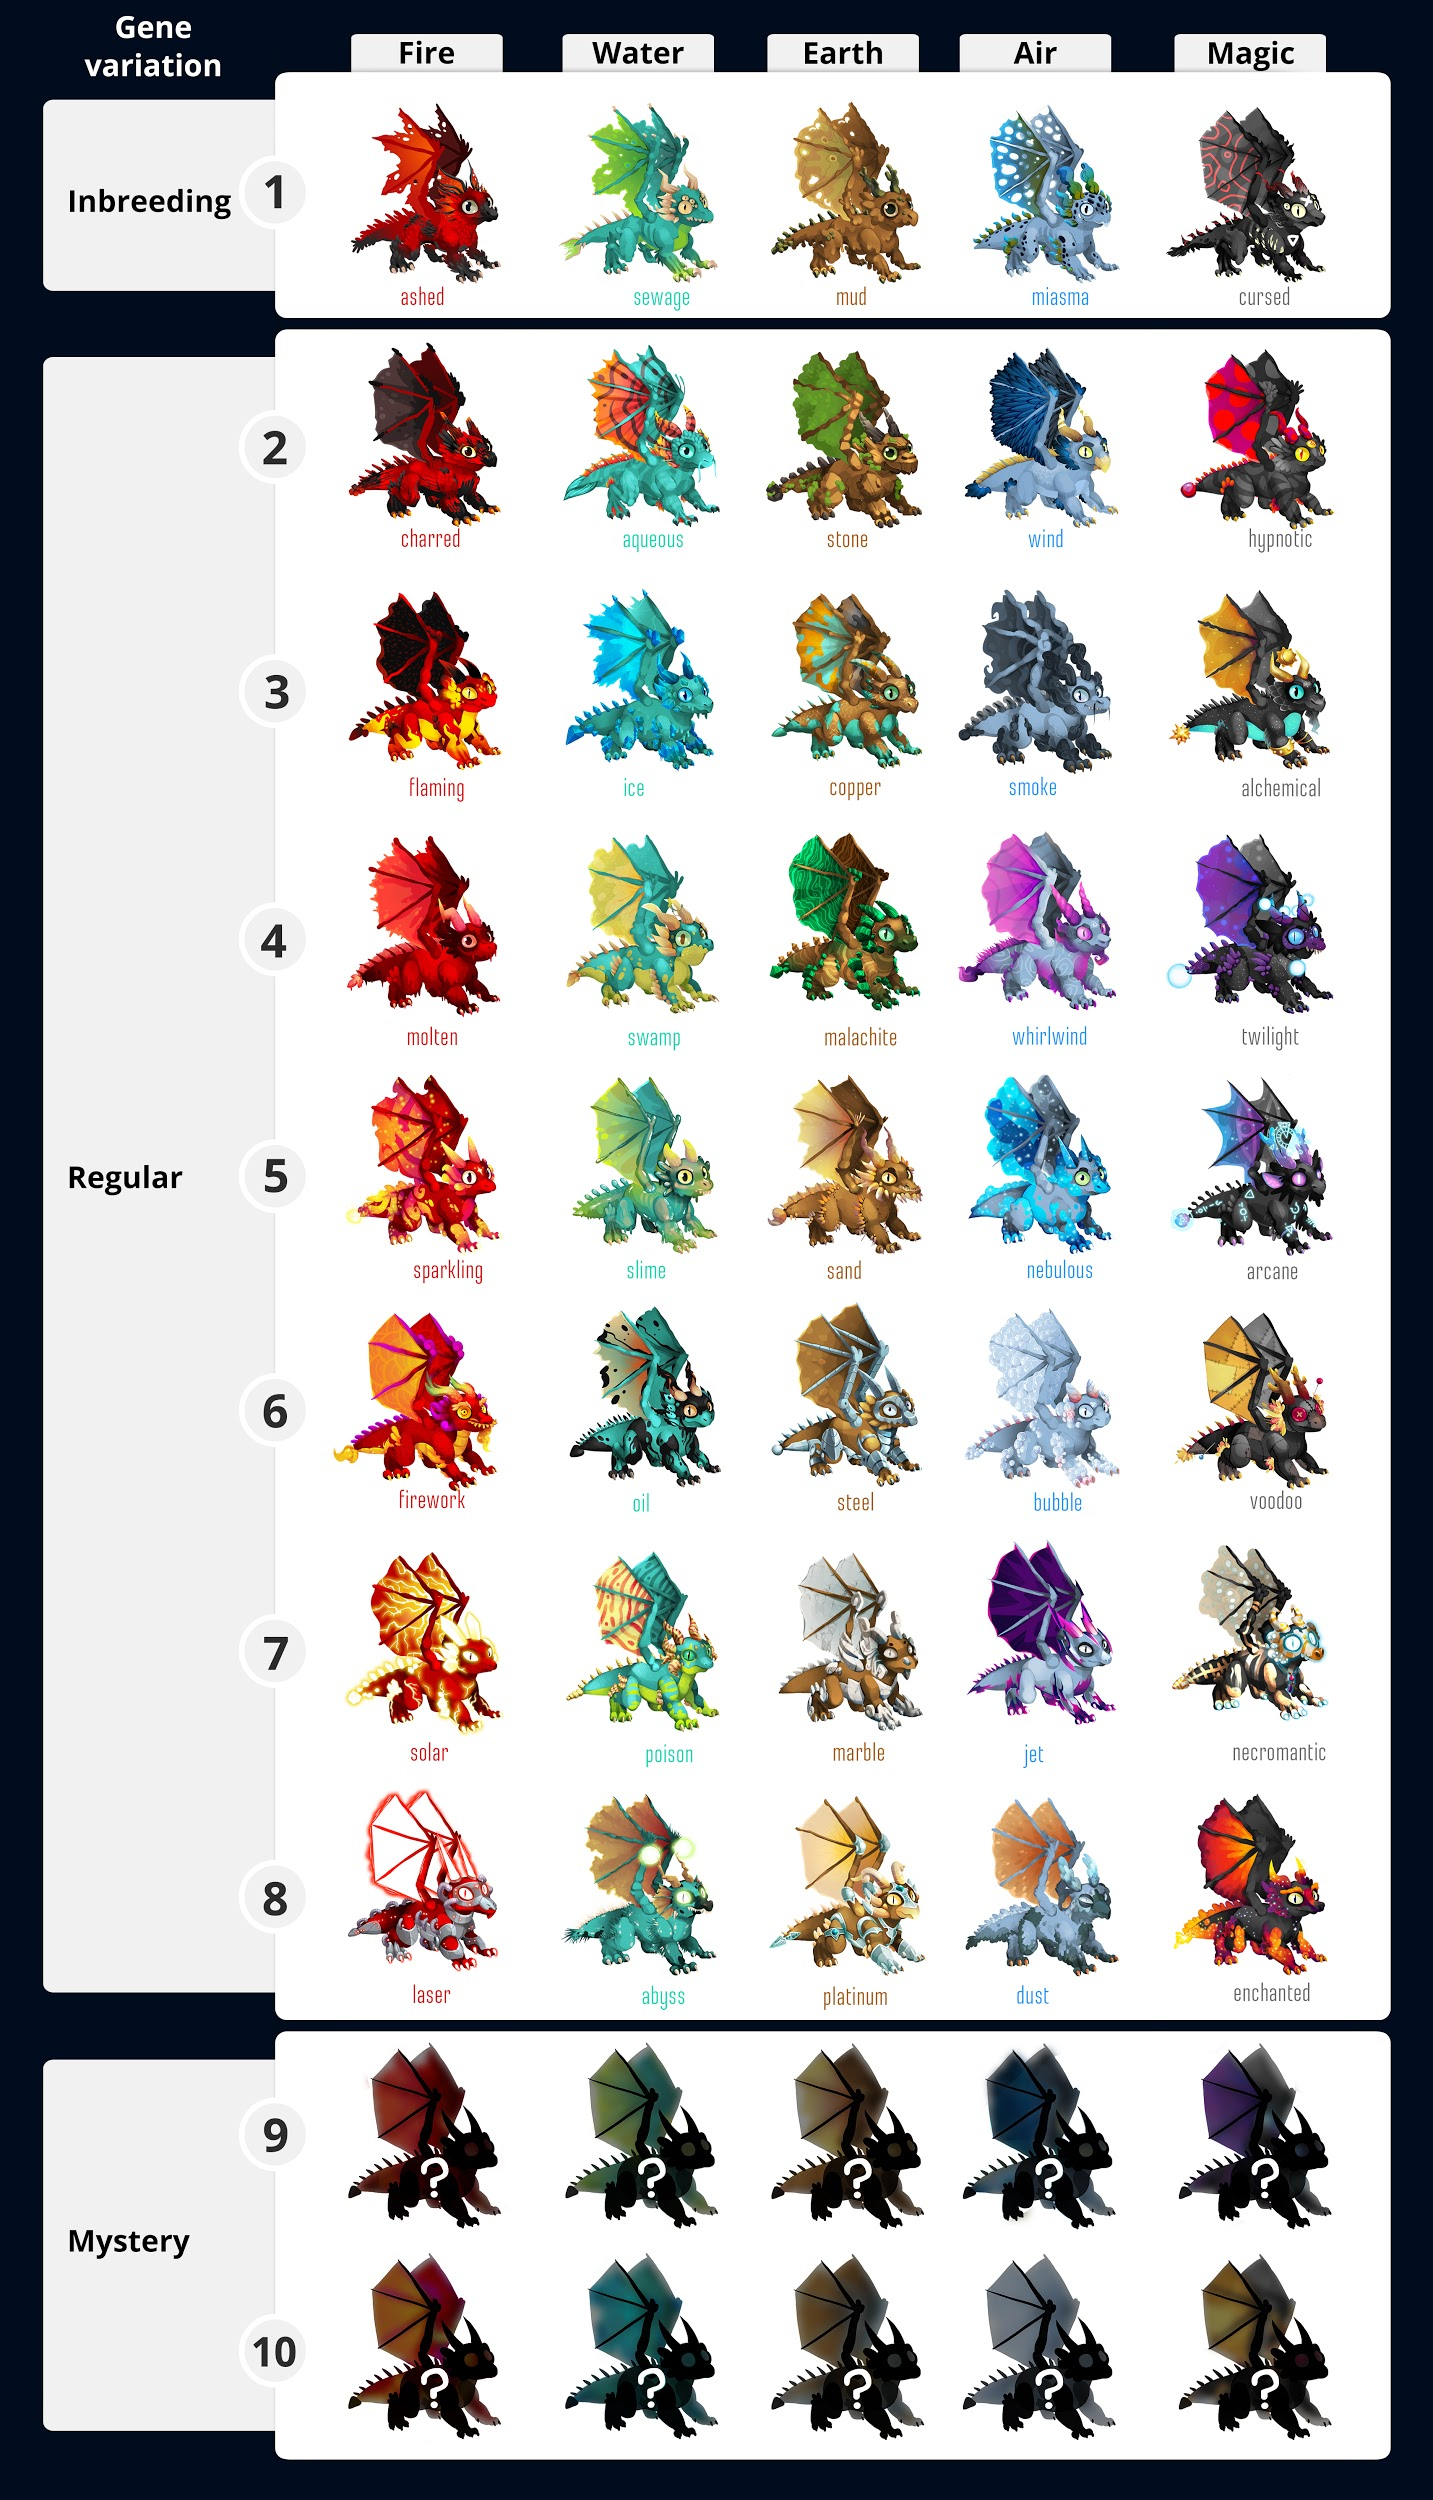
\includegraphics[width=4.85in,height=8.48in]{./media/image14.jpg}
		\caption{The different dragon types, with all of their possible variations, including inbreeding - row 1, regular rows 2-8, and mystery rows 9, and 10.}
		\label{fig:The_different_dragon_types_with_all_of_their_possible_variations_including_inbreeding_row_1_regular_rows_28_and_mystery_rows_9_and_10}
	\end{Center}
\end{figure}


%%%%%%%%%%%%%%%%%%%% Figure/Image No: 3 Ends here %%%%%%%%%%%%%%%%%%%%



\end{Center}\par


Five different dragon types will be released during Dragonereum’s launch. Each type will inherit Regular genes according to the gene variety Table shown in Figure  \ref{fig:The_different_dragon_types_with_all_of_their_possible_variations_including_inbreeding_row_1_regular_rows_28_and_mystery_rows_9_and_10}.  There will be 10000 genesis eggs released during the Genesis. Inbreeding genes and genes of highest quality (Mystery Genes) will play no part in the genesis dragon creation process.\par

Since every dragon has ten different body parts, each dragon type has 282 475 249 (7\textsuperscript{10}) different dragon varieties. This is not including Inbreeding and Mystery Genes. Therefore, the chance of receiving two similar dragons during Genesis is 0.000708026634928287$\%$  (1 in 141 237). Consequently, we do not do additional checks for the existence of a particular dragon appearance as chances are very small but this check will require additional gas usage by the smart contract.\par

Five types of dragons will result in 2 758 547 353 515 625 different breeds when combined. Again, that is without inbreeding and Mystery genes. If all those dragons are to be evenly distributed among the population of the Earth, each person would receive around 360 000 varieties of dragons.\par

Together with inbreeding and Mystery Genes, there will be 97 656 250 000 000 000 different dragons originating from those initial five types. This is 12 800 000 for each person in the World.

 %%%%%%%%%%%%  Starting New Page here %%%%%%%%%%%%%%

\newpage
\par

\section{Game Mechanics}
%\addcontentsline{toc}{section}{Game Mechanics}
 \label{Game Mechanics}  \par
 
Our aim is to create a cryptocollectible game, whereby those users who spend more time playing the game have the possibility to own higher valued dragons and accumulate higher amounts of Gold.\par

In order to do this the game ecosystem should be balanced and should meet the following criteria:\par

\begin{itemize}
	\item The growth of the dragon population should be limited by the game mechanics.\par

	\item Early game adopters should have an advantage in accumulating Gold over those players who joined the game at a later date, given that all other comparing factors are on an equal footing.\par

	\item There should not be one winning strategy that will allow someone to gain advantage over other players.
\end{itemize}\par

In this section we address these issues and explain the solutions that are implemented in order to comply with those requirements.\par

However, before we do this we have to get a deeper understanding of the game mechanics and underlying math. We have explained some game concepts in Section \ref{Introduction to Dragonereum}, and here we will dig into the details and formulas.\par

\subsection{Body parts and basic skills}
%\addcontentsline{toc}{subsection}{Body parts and basic skills}
\label{Body parts and basic skills}  \par

As it was discussed, there are five Basic Skills: \textit{attack}, \textit{defense}, \textit{stamina}, \textit{speed}, and \textit{intelligence}. The basic skills are calculated based on the dragon’s genetics and obtained experience (body parts level ups).\par

\begin{itemize}
	\item \textit{Attack} -- affects the degree of damage a dragon can cause in a battle.\par

	\item \textit{Defense} -- measures the ability of a dragon to defend itself during a battle. If the dragon engages in a battle with a dragon which has less \textit{attack}, \textit{defense} determines the damage it can do to the weaker attacking dragon.\par

	\item \textit{Stamina -- }measures the maximum amount of HP and the speed of regeneration.\par

	\item \textit{Speed} -- defines which dragon moves first and each dragon’s maximum reach.\par

	\item \textit{Intelligence -- }determines the maximum amount of Mana, along with \textit{speed} for regeneration and the probability of \textit{special attack} or \textit{special defense} being used in battles.
\end{itemize}\par

The total skills of a dragon are calculated by summing up all body parts increased by Level Ups. So if you upgrade the wings of a dragon, the total skills of a dragon will also receive a boost.\par

As it was noted in Section \ref{Blockchain breeding algorithm} each dragon has ten body parts. Each body part is responsible for three particular basic skills and it does not contribute to the remaining two, see  Table \ref{tab:The table shows which body parts are responsible for which particular skills.}.\par




%%%%%%%%%%%%%%%%%%%% Table No: 1 starts here %%%%%%%%%%%%%%%%%%%%


\begin{table}[!ht]
 			\centering
\begin{tabular}{p{0.84in}p{0.84in}p{0.84in}p{0.84in}p{0.84in}p{0.84in}}
\hhline{~-----}
%row no:1
\multicolumn{1}{p{0.84in}|}{} & 
\multicolumn{1}{p{0.84in}|}{\Centering {\fontsize{10pt}{12.0pt}\selectfont Attack}} & 
\multicolumn{1}{p{0.84in}|}{\Centering {\fontsize{10pt}{12.0pt}\selectfont Defense}} & 
\multicolumn{1}{p{0.84in}|}{\Centering {\fontsize{10pt}{12.0pt}\selectfont Stamina}} & 
\multicolumn{1}{p{0.84in}|}{\Centering {\fontsize{10pt}{12.0pt}\selectfont Speed}} & 
\multicolumn{1}{p{0.84in}|}{\Centering {\fontsize{10pt}{12.0pt}\selectfont Intelligence}} \\
\hhline{------}
%row no:2
\multicolumn{1}{|p{0.84in}|}{{\fontsize{10pt}{12.0pt}\selectfont Head}} & 
\multicolumn{1}{p{0.84in}|}{\Centering {\( \checkmark \)}} & 
\multicolumn{1}{p{0.84in}|}{\Centering {\fontsize{10pt}{12.0pt}\selectfont  $\times$  }} & 
\multicolumn{1}{p{0.84in}|}{\Centering {\( \checkmark \)}} & 
\multicolumn{1}{p{0.84in}|}{\Centering {\fontsize{10pt}{12.0pt}\selectfont  $\times$  }} & 
\multicolumn{1}{p{0.84in}|}{\Centering {\( \checkmark \)}} \\
\hhline{------}
%row no:3
\multicolumn{1}{|p{0.84in}|}{{\fontsize{10pt}{12.0pt}\selectfont Eyes}} & 
\multicolumn{1}{p{0.84in}|}{\Centering {\fontsize{10pt}{12.0pt}\selectfont  $\times$  }} & 
\multicolumn{1}{p{0.84in}|}{\Centering {\( \checkmark \)}} & 
\multicolumn{1}{p{0.84in}|}{\Centering {\fontsize{10pt}{12.0pt}\selectfont  $\times$  }} & 
\multicolumn{1}{p{0.84in}|}{\Centering {\( \checkmark \)}} & 
\multicolumn{1}{p{0.84in}|}{\Centering {\( \checkmark \)}} \\
\hhline{------}
%row no:4
\multicolumn{1}{|p{0.84in}|}{{\fontsize{10pt}{12.0pt}\selectfont Horns}} & 
\multicolumn{1}{p{0.84in}|}{\Centering {\( \checkmark \)}} & 
\multicolumn{1}{p{0.84in}|}{\Centering {\( \checkmark \)}} & 
\multicolumn{1}{p{0.84in}|}{\Centering {\fontsize{10pt}{12.0pt}\selectfont  $\times$  }} & 
\multicolumn{1}{p{0.84in}|}{\Centering {\fontsize{10pt}{12.0pt}\selectfont  $\times$  }} & 
\multicolumn{1}{p{0.84in}|}{\Centering {\( \checkmark \)}} \\
\hhline{------}
%row no:5
\multicolumn{1}{|p{0.84in}|}{{\fontsize{10pt}{12.0pt}\selectfont Body}} & 
\multicolumn{1}{p{0.84in}|}{\Centering {\( \checkmark \)}} & 
\multicolumn{1}{p{0.84in}|}{\Centering {\( \checkmark \)}} & 
\multicolumn{1}{p{0.84in}|}{\Centering {\( \checkmark \)}} & 
\multicolumn{1}{p{0.84in}|}{\Centering {\fontsize{10pt}{12.0pt}\selectfont  $\times$  }} & 
\multicolumn{1}{p{0.84in}|}{\Centering {\fontsize{10pt}{12.0pt}\selectfont  $\times$  }} \\
\hhline{------}
%row no:6
\multicolumn{1}{|p{0.84in}|}{{\fontsize{10pt}{12.0pt}\selectfont Wings}} & 
\multicolumn{1}{p{0.84in}|}{\Centering {\fontsize{10pt}{12.0pt}\selectfont  $\times$  }} & 
\multicolumn{1}{p{0.84in}|}{\Centering {\fontsize{10pt}{12.0pt}\selectfont  $\times$  }} & 
\multicolumn{1}{p{0.84in}|}{\Centering {\( \checkmark \)}} & 
\multicolumn{1}{p{0.84in}|}{\Centering {\( \checkmark \)}} & 
\multicolumn{1}{p{0.84in}|}{\Centering {\( \checkmark \)}} \\
\hhline{------}
%row no:7
\multicolumn{1}{|p{0.84in}|}{{\fontsize{10pt}{12.0pt}\selectfont Arms}} & 
\multicolumn{1}{p{0.84in}|}{\Centering {\( \checkmark \)}} & 
\multicolumn{1}{p{0.84in}|}{\Centering {\fontsize{10pt}{12.0pt}\selectfont  $\times$  }} & 
\multicolumn{1}{p{0.84in}|}{\Centering {\( \checkmark \)}} & 
\multicolumn{1}{p{0.84in}|}{\Centering {\( \checkmark \)}} & 
\multicolumn{1}{p{0.84in}|}{\Centering {\fontsize{10pt}{12.0pt}\selectfont  $\times$  }} \\
\hhline{------}
%row no:8
\multicolumn{1}{|p{0.84in}|}{{\fontsize{10pt}{12.0pt}\selectfont Legs}} & 
\multicolumn{1}{p{0.84in}|}{\Centering {\fontsize{10pt}{12.0pt}\selectfont  $\times$  }}& 
\multicolumn{1}{p{0.84in}|}{\Centering {\( \checkmark \)}} & 
\multicolumn{1}{p{0.84in}|}{\Centering {\( \checkmark \)}} & 
\multicolumn{1}{p{0.84in}|}{\Centering {\( \checkmark \)}} & 
\multicolumn{1}{p{0.84in}|}{\Centering {\fontsize{10pt}{12.0pt}\selectfont  $\times$  }} \\
\hhline{------}
%row no:9
\multicolumn{1}{|p{0.84in}|}{{\fontsize{10pt}{12.0pt}\selectfont Tail}} & 
\multicolumn{1}{p{0.84in}|}{\Centering {\( \checkmark \)}} & 
\multicolumn{1}{p{0.84in}|}{\Centering {\fontsize{10pt}{12.0pt}\selectfont  $\times$  }} & 
\multicolumn{1}{p{0.84in}|}{\Centering {\( \checkmark \)}} & 
\multicolumn{1}{p{0.84in}|}{\Centering {\( \checkmark \)}} & 
\multicolumn{1}{p{0.84in}|}{\Centering {\fontsize{10pt}{12.0pt}\selectfont  $\times$  }} \\
\hhline{------}
%row no:10
\multicolumn{1}{|p{0.84in}|}{{\fontsize{10pt}{12.0pt}\selectfont Spike}} & 
\multicolumn{1}{p{0.84in}|}{\Centering {\( \checkmark \)}} & 
\multicolumn{1}{p{0.84in}|}{\Centering {\( \checkmark \)}} & 
\multicolumn{1}{p{0.84in}|}{\Centering {\fontsize{10pt}{12.0pt}\selectfont  $\times$  }} & 
\multicolumn{1}{p{0.84in}|}{\Centering {\fontsize{10pt}{12.0pt}\selectfont  $\times$  }} & 
\multicolumn{1}{p{0.84in}|}{\Centering {\( \checkmark \)}} \\
\hhline{------}
%row no:11
\multicolumn{1}{|p{0.84in}|}{{\fontsize{10pt}{12.0pt}\selectfont Pattern}} & 
\multicolumn{1}{p{0.84in}|}{\Centering {\fontsize{10pt}{12.0pt}\selectfont  $\times$  }} & 
\multicolumn{1}{p{0.84in}|}{\Centering {\( \checkmark \)}} & 
\multicolumn{1}{p{0.84in}|}{\Centering {\fontsize{10pt}{12.0pt}\selectfont  $\times$  }} & 
\multicolumn{1}{p{0.84in}|}{\Centering {\( \checkmark \)}} & 
\multicolumn{1}{p{0.84in}|}{\Centering {\( \checkmark \)}} \\
\hhline{------}

\end{tabular}\caption{The table shows which body parts are responsible for which particular skills.}
\label{tab:The table shows which body parts are responsible for which particular skills.}

 \end{table}


%%%%%%%%%%%%%%%%%%%% Table No: 1 ends here %%%%%%%%%%%%%%%%%%%%


\subsection{Dragon types/families}
%\addcontentsline{toc}{subsection}{Dragon types/families}
\label{Dragon types/families}  \par

A dragon might have a combination of body parts of different types and varieties depending on the genome of the particular dragon.\par

Each dragon type/family is better at a particular basic skill, as shown in  Table \ref{tab:The dragon type factor for each basic skill.}. For example, fire dragons have more \textit{attack} compared to other dragon families.\par



%%%%%%%%%%%%%%%%%%%% Table No: 2 starts here %%%%%%%%%%%%%%%%%%%%


\begin{table}[!ht]
 			\centering
\begin{tabular}{p{0.84in}p{0.84in}p{0.84in}p{0.84in}p{0.84in}p{0.84in}}
\hhline{~-----}
%row no:1
\multicolumn{1}{p{0.84in}|}{} & 
\multicolumn{1}{p{0.84in}|}{\Centering {\fontsize{10pt}{12.0pt}\selectfont Attack}} & 
\multicolumn{1}{p{0.84in}|}{\Centering {\fontsize{10pt}{12.0pt}\selectfont Defense}} & 
\multicolumn{1}{p{0.84in}|}{\Centering {\fontsize{10pt}{12.0pt}\selectfont Stamina}} & 
\multicolumn{1}{p{0.84in}|}{\Centering {\fontsize{10pt}{12.0pt}\selectfont Speed}} & 
\multicolumn{1}{p{0.84in}|}{\Centering {\fontsize{10pt}{12.0pt}\selectfont Intelligence}} \\
\hhline{------}
%row no:2
\multicolumn{1}{|p{0.84in}|}{{\fontsize{10pt}{12.0pt}\selectfont Fire}} & 
\multicolumn{1}{p{0.84in}|}{\Centering {\fontsize{10pt}{12.0pt}\selectfont 1.5}} & 
\multicolumn{1}{p{0.84in}|}{\Centering {\fontsize{10pt}{12.0pt}\selectfont 1}} & 
\multicolumn{1}{p{0.84in}|}{\Centering {\fontsize{10pt}{12.0pt}\selectfont 1}} & 
\multicolumn{1}{p{0.84in}|}{\Centering {\fontsize{10pt}{12.0pt}\selectfont 1}} & 
\multicolumn{1}{p{0.84in}|}{\Centering {\fontsize{10pt}{12.0pt}\selectfont 1}} \\
\hhline{------}
%row no:3
\multicolumn{1}{|p{0.84in}|}{{\fontsize{10pt}{12.0pt}\selectfont Water}} & 
\multicolumn{1}{p{0.84in}|}{\Centering {\fontsize{10pt}{12.0pt}\selectfont 1}} & 
\multicolumn{1}{p{0.84in}|}{\Centering {\fontsize{10pt}{12.0pt}\selectfont 1}} & 
\multicolumn{1}{p{0.84in}|}{\Centering {\fontsize{10pt}{12.0pt}\selectfont 1.5}} & 
\multicolumn{1}{p{0.84in}|}{\Centering {\fontsize{10pt}{12.0pt}\selectfont 1}} & 
\multicolumn{1}{p{0.84in}|}{\Centering {\fontsize{10pt}{12.0pt}\selectfont 1}} \\
\hhline{------}
%row no:4
\multicolumn{1}{|p{0.84in}|}{{\fontsize{10pt}{12.0pt}\selectfont Earth}} & 
\multicolumn{1}{p{0.84in}|}{\Centering {\fontsize{10pt}{12.0pt}\selectfont 1}} & 
\multicolumn{1}{p{0.84in}|}{\Centering {\fontsize{10pt}{12.0pt}\selectfont 1.5}} & 
\multicolumn{1}{p{0.84in}|}{\Centering {\fontsize{10pt}{12.0pt}\selectfont 1}} & 
\multicolumn{1}{p{0.84in}|}{\Centering {\fontsize{10pt}{12.0pt}\selectfont 1}} & 
\multicolumn{1}{p{0.84in}|}{\Centering {\fontsize{10pt}{12.0pt}\selectfont 1}} \\
\hhline{------}
%row no:5
\multicolumn{1}{|p{0.84in}|}{{\fontsize{10pt}{12.0pt}\selectfont Air}} & 
\multicolumn{1}{p{0.84in}|}{\Centering {\fontsize{10pt}{12.0pt}\selectfont 1}} & 
\multicolumn{1}{p{0.84in}|}{\Centering {\fontsize{10pt}{12.0pt}\selectfont 1}} & 
\multicolumn{1}{p{0.84in}|}{\Centering {\fontsize{10pt}{12.0pt}\selectfont 1}} & 
\multicolumn{1}{p{0.84in}|}{\Centering {\fontsize{10pt}{12.0pt}\selectfont 1.5}} & 
\multicolumn{1}{p{0.84in}|}{\Centering {\fontsize{10pt}{12.0pt}\selectfont 1}} \\
\hhline{------}
%row no:6
\multicolumn{1}{|p{0.84in}|}{{\fontsize{10pt}{12.0pt}\selectfont Cyber}} & 
\multicolumn{1}{p{0.84in}|}{\Centering {\fontsize{10pt}{12.0pt}\selectfont 1}} & 
\multicolumn{1}{p{0.84in}|}{\Centering {\fontsize{10pt}{12.0pt}\selectfont 1}} & 
\multicolumn{1}{p{0.84in}|}{\Centering {\fontsize{10pt}{12.0pt}\selectfont 1}} & 
\multicolumn{1}{p{0.84in}|}{\Centering {\fontsize{10pt}{12.0pt}\selectfont 1}} & 
\multicolumn{1}{p{0.84in}|}{\Centering {\fontsize{10pt}{12.0pt}\selectfont 1.5}} \\
\hhline{------}

\end{tabular}\caption{The dragon type factor for each basic skill.}
\label{tab:The dragon type factor for each basic skill.}

 \end{table}


%%%%%%%%%%%%%%%%%%%% Table No: 2 ends here %%%%%%%%%%%%%%%%%%%%

Additionally, every dragon type has a unique advantage (in the form of higher damage) over other dragon types, similar to the $``$rock-paper-scissors$"$  game, as shown in Figure \ref{fig:Fire}. For example, water dragons will generally outperform fire dragons as water puts out fire.\par



%%%%%%%%%%%%%%%%%%%% Figure/Image No: 4 starts here %%%%%%%%%%%%%%%%%%%%

\begin{figure}[!ht]
	\begin{Center}
		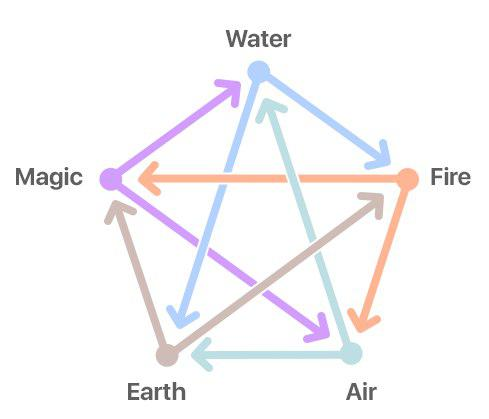
\includegraphics[width=3.32in,height=2.84in]{./media/image22.jpg}
		\caption{Each dragon family has an advantage over the two dragon families towards which the arrows are pointed: water over earth and fire, fire over air and cyber, air over earth and water, earth over cyber and fire, and cyber over water and air.} 
		\label{fig:Fire}
	\end{Center}
\end{figure}


%%%%%%%%%%%%%%%%%%%% Figure/Image No: 4 Ends here %%%%%%%%%%%%%%%%%%%%

\par

Also, each dragon family has a particular \textit{special attack, special defense} and \textit{special peaceful skill}.\par


\subsection{Dragon varieties}
%\addcontentsline{toc}{subsection}{Dragon varieties}
\label{Dragon varieties}  \par

Each dragon family has genes of different quality. The differences between these varieties influence the dragon’s appearance and strength of skills. Therefore, one water dragon might be stronger than another water dragon even without updates or leveling up.\par

The appearance was already displayed in Figure  \ref{fig:The_different_dragon_types_with_all_of_their_possible_variations_including_inbreeding_row_1_regular_rows_28_and_mystery_rows_9_and_10} of Section \ref{Dragon diversity}, and here we discuss the skills of the different varieties.\par

 Table \ref{tab: The dragon variety factors for each basic skills depending on the dragon gene variation.} below provides the dragon variety factors for the five basic skills depending on the different dragon varieties \par



%%%%%%%%%%%%%%%%%%%% Table No: 3 starts here %%%%%%%%%%%%%%%%%%%%


\begin{table}[!ht]
 			\centering
\begin{tabular}{p{0.84in}p{0.65in}p{0.68in}p{0.68in}p{0.68in}p{0.68in}p{0.68in}}
\hhline{-------}
%row no:1
\multicolumn{1}{|p{0.84in}|}{{\fontsize{10pt}{12.0pt}\selectfont Variety}} & 
\multicolumn{1}{p{0.65in}|}{{\fontsize{10pt}{12.0pt}\selectfont Codename}} & 
\multicolumn{1}{p{0.68in}|}{\Centering {\fontsize{10pt}{12.0pt}\selectfont Attack}} & 
\multicolumn{1}{p{0.68in}|}{\Centering {\fontsize{10pt}{12.0pt}\selectfont Defense}} & 
\multicolumn{1}{p{0.68in}|}{\Centering {\fontsize{10pt}{12.0pt}\selectfont Stamina}} & 
\multicolumn{1}{p{0.68in}|}{\Centering {\fontsize{10pt}{12.0pt}\selectfont Speed}} & 
\multicolumn{1}{p{0.68in}|}{\Centering {\fontsize{10pt}{12.0pt}\selectfont Intelligence}} \\
\hhline{-------}
%row no:2
\multicolumn{1}{|p{0.84in}|}{{\fontsize{10pt}{12.0pt}\selectfont 1 (inbreeding)}} & 
\multicolumn{1}{p{0.65in}|}{{\fontsize{10pt}{12.0pt}\selectfont Inbreeding}} & 
\multicolumn{1}{p{0.68in}|}{\Centering {\fontsize{10pt}{12.0pt}\selectfont 0.5}} & 
\multicolumn{1}{p{0.68in}|}{\Centering {\fontsize{10pt}{12.0pt}\selectfont 0.5}} & 
\multicolumn{1}{p{0.68in}|}{\Centering {\fontsize{10pt}{12.0pt}\selectfont 0.5}} & 
\multicolumn{1}{p{0.68in}|}{\Centering {\fontsize{10pt}{12.0pt}\selectfont 0.5}} & 
\multicolumn{1}{p{0.68in}|}{\Centering {\fontsize{10pt}{12.0pt}\selectfont 0.5}} \\
\hhline{-------}
%row no:3
\multicolumn{1}{|p{0.84in}|}{{\fontsize{10pt}{12.0pt}\selectfont 2 (regular)}} & 
\multicolumn{1}{p{0.65in}|}{{\fontsize{10pt}{12.0pt}\selectfont Common 0}} & 
\multicolumn{1}{p{0.68in}|}{\Centering {\fontsize{10pt}{12.0pt}\selectfont 1.5}} & 
\multicolumn{1}{p{0.68in}|}{\Centering {\fontsize{10pt}{12.0pt}\selectfont 1.5}} & 
\multicolumn{1}{p{0.68in}|}{\Centering {\fontsize{10pt}{12.0pt}\selectfont 1}} & 
\multicolumn{1}{p{0.68in}|}{\Centering {\fontsize{10pt}{12.0pt}\selectfont 1}} & 
\multicolumn{1}{p{0.68in}|}{\Centering {\fontsize{10pt}{12.0pt}\selectfont 1}} \\
\hhline{-------}
%row no:4
\multicolumn{1}{|p{0.84in}|}{{\fontsize{10pt}{12.0pt}\selectfont 3 (regular)}} & 
\multicolumn{1}{p{0.65in}|}{{\fontsize{10pt}{12.0pt}\selectfont Common 1}} & 
\multicolumn{1}{p{0.68in}|}{\Centering {\fontsize{10pt}{12.0pt}\selectfont 1}} & 
\multicolumn{1}{p{0.68in}|}{\Centering {\fontsize{10pt}{12.0pt}\selectfont 1.5}} & 
\multicolumn{1}{p{0.68in}|}{\Centering {\fontsize{10pt}{12.0pt}\selectfont 1.5}} & 
\multicolumn{1}{p{0.68in}|}{\Centering {\fontsize{10pt}{12.0pt}\selectfont 1}} & 
\multicolumn{1}{p{0.68in}|}{\Centering {\fontsize{10pt}{12.0pt}\selectfont 1}} \\
\hhline{-------}
%row no:5
\multicolumn{1}{|p{0.84in}|}{{\fontsize{10pt}{12.0pt}\selectfont 4 (regular)}} & 
\multicolumn{1}{p{0.65in}|}{{\fontsize{10pt}{12.0pt}\selectfont Common 2}} & 
\multicolumn{1}{p{0.68in}|}{\Centering {\fontsize{10pt}{12.0pt}\selectfont 1}} & 
\multicolumn{1}{p{0.68in}|}{\Centering {\fontsize{10pt}{12.0pt}\selectfont 1}} & 
\multicolumn{1}{p{0.68in}|}{\Centering {\fontsize{10pt}{12.0pt}\selectfont 1.5}} & 
\multicolumn{1}{p{0.68in}|}{\Centering {\fontsize{10pt}{12.0pt}\selectfont 1.5}} & 
\multicolumn{1}{p{0.68in}|}{\Centering {\fontsize{10pt}{12.0pt}\selectfont 1}} \\
\hhline{-------}
%row no:6
\multicolumn{1}{|p{0.84in}|}{{\fontsize{10pt}{12.0pt}\selectfont 5 (regular)}} & 
\multicolumn{1}{p{0.65in}|}{{\fontsize{10pt}{12.0pt}\selectfont Common 3}} & 
\multicolumn{1}{p{0.68in}|}{\Centering {\fontsize{10pt}{12.0pt}\selectfont 1}} & 
\multicolumn{1}{p{0.68in}|}{\Centering {\fontsize{10pt}{12.0pt}\selectfont 1}} & 
\multicolumn{1}{p{0.68in}|}{\Centering {\fontsize{10pt}{12.0pt}\selectfont 1}} & 
\multicolumn{1}{p{0.68in}|}{\Centering {\fontsize{10pt}{12.0pt}\selectfont 1.5}} & 
\multicolumn{1}{p{0.68in}|}{\Centering {\fontsize{10pt}{12.0pt}\selectfont 1.5}} \\
\hhline{-------}
%row no:7
\multicolumn{1}{|p{0.84in}|}{{\fontsize{10pt}{12.0pt}\selectfont 6 (regular)}} & 
\multicolumn{1}{p{0.65in}|}{{\fontsize{10pt}{12.0pt}\selectfont Rare 0}} & 
\multicolumn{1}{p{0.68in}|}{\Centering {\fontsize{10pt}{12.0pt}\selectfont 2}} & 
\multicolumn{1}{p{0.68in}|}{\Centering {\fontsize{10pt}{12.0pt}\selectfont 2}} & 
\multicolumn{1}{p{0.68in}|}{\Centering {\fontsize{10pt}{12.0pt}\selectfont 2}} & 
\multicolumn{1}{p{0.68in}|}{\Centering {\fontsize{10pt}{12.0pt}\selectfont 1}} & 
\multicolumn{1}{p{0.68in}|}{\Centering {\fontsize{10pt}{12.0pt}\selectfont 1}} \\
\hhline{-------}
%row no:8
\multicolumn{1}{|p{0.84in}|}{{\fontsize{10pt}{12.0pt}\selectfont 7 (regular)}} & 
\multicolumn{1}{p{0.65in}|}{{\fontsize{10pt}{12.0pt}\selectfont Rare 1}} & 
\multicolumn{1}{p{0.68in}|}{\Centering {\fontsize{10pt}{12.0pt}\selectfont 1}} & 
\multicolumn{1}{p{0.68in}|}{\Centering {\fontsize{10pt}{12.0pt}\selectfont 2}} & 
\multicolumn{1}{p{0.68in}|}{\Centering {\fontsize{10pt}{12.0pt}\selectfont 2}} & 
\multicolumn{1}{p{0.68in}|}{\Centering {\fontsize{10pt}{12.0pt}\selectfont 2}} & 
\multicolumn{1}{p{0.68in}|}{\Centering {\fontsize{10pt}{12.0pt}\selectfont 1}} \\
\hhline{-------}
%row no:9
\multicolumn{1}{|p{0.84in}|}{{\fontsize{10pt}{12.0pt}\selectfont 8 (regular)}} & 
\multicolumn{1}{p{0.65in}|}{{\fontsize{10pt}{12.0pt}\selectfont Rare 2}} & 
\multicolumn{1}{p{0.68in}|}{\Centering {\fontsize{10pt}{12.0pt}\selectfont 1}} & 
\multicolumn{1}{p{0.68in}|}{\Centering {\fontsize{10pt}{12.0pt}\selectfont 1}} & 
\multicolumn{1}{p{0.68in}|}{\Centering {\fontsize{10pt}{12.0pt}\selectfont 2}} & 
\multicolumn{1}{p{0.68in}|}{\Centering {\fontsize{10pt}{12.0pt}\selectfont 2}} & 
\multicolumn{1}{p{0.68in}|}{\Centering {\fontsize{10pt}{12.0pt}\selectfont 2}} \\
\hhline{-------}
%row no:10
\multicolumn{1}{|p{0.84in}|}{{\fontsize{10pt}{12.0pt}\selectfont 9 (mystery)}} & 
\multicolumn{1}{p{0.65in}|}{{\fontsize{10pt}{12.0pt}\selectfont Epic 0}} & 
\multicolumn{1}{p{0.68in}|}{\Centering {\fontsize{10pt}{12.0pt}\selectfont 4}} & 
\multicolumn{1}{p{0.68in}|}{\Centering {\fontsize{10pt}{12.0pt}\selectfont 4}} & 
\multicolumn{1}{p{0.68in}|}{\Centering {\fontsize{10pt}{12.0pt}\selectfont 4}} & 
\multicolumn{1}{p{0.68in}|}{\Centering {\fontsize{10pt}{12.0pt}\selectfont 1}} & 
\multicolumn{1}{p{0.68in}|}{\Centering {\fontsize{10pt}{12.0pt}\selectfont 1}} \\
\hhline{-------}
%row no:11
\multicolumn{1}{|p{0.84in}|}{{\fontsize{10pt}{12.0pt}\selectfont 10 (mystery)}} & 
\multicolumn{1}{p{0.65in}|}{{\fontsize{10pt}{12.0pt}\selectfont Epic 1}} & 
\multicolumn{1}{p{0.68in}|}{\Centering {\fontsize{10pt}{12.0pt}\selectfont 1}} & 
\multicolumn{1}{p{0.68in}|}{\Centering {\fontsize{10pt}{12.0pt}\selectfont 1}} & 
\multicolumn{1}{p{0.68in}|}{\Centering {\fontsize{10pt}{12.0pt}\selectfont 4}} & 
\multicolumn{1}{p{0.68in}|}{\Centering {\fontsize{10pt}{12.0pt}\selectfont 4}} & 
\multicolumn{1}{p{0.68in}|}{\Centering {\fontsize{10pt}{12.0pt}\selectfont 4}} \\
\hhline{-------}

\end{tabular}\caption{The dragon variety factors for each basic skills depending on the dragon gene variation.}
\label{tab: The dragon variety factors for each basic skills depending on the dragon gene variation.}

 \end{table}


%%%%%%%%%%%%%%%%%%%% Table No: 3 ends here %%%%%%%%%%%%%%%%%%%%

In  Table \ref{tab: The dragon variety factors for each basic skills depending on the dragon gene variation.}, the first row shows the dragon variety factor for inbreeding dragons, as such it is penalized by our genetics algorithm to be 0.5.\par

The genes of the highest quality (9–10 in  Table \ref{tab: The dragon variety factors for each basic skills depending on the dragon gene variation.} above) are Mystery Genes and will only be accessible as a result of mutations. Genesis dragons will not have these genes at all (more on it in Section \ref{Genesis}).\par

The chance for a regular mutation to occur (excluding the case when two relatives interbreed) can be described as follows:\par

\begin{itemize}
  \begin{samepage}
	\item During the incubation there is a 10$\%$  probability for each gene to mutate.\par

	\item The mutated gene might be of any of the varieties between 2 (regular) and 10 (mystery) listed in column 1 of  Table \ref{tab: The dragon variety factors for each basic skills depending on the dragon gene variation.} with an equal probability (the 1 (Inbreeding) variety is received only in the case when close relatives interbreed).\par
  \end{samepage}
\end{itemize}

Details of inbreeding penalties and chances are described in our Medium  \mbox{articles (\url{https://medium.com/@dragonereum})}. \par

If a player chooses to inbreed close relatives there is a high probability for a negative mutation will occur. This probability depends on different cases and is:\par

\begin{itemize}
  \begin{samepage}
	\item Very high for inbreeding full siblings (80$\%$ )\par

	\item High for inbreeding half-siblings (70$\%$ )\par

	\item 50$\%$  for second and third cousins. The chances of negative mutations might increase if these dragons have several close relatives. 
  \end{samepage}
\end{itemize}\par

\subsection{Calculating the overall basic skills of a dragon}
%\addcontentsline{toc}{subsection}{Calculating the overall basic skills of a dragon}
\label{Calculating the overall basic skills of a dragon}  \par

The overall skills of a dragon will be calculated as the sum of skills for all its body parts:
\begin{center}
   \begin{equation}
   \label{Eq:Sk}
      Sk(j) = \sum_{i=1}^{10} bp^i(j)*f_{dt}^i(j)*f_{dv}^i(j)*L^i,
   \end{equation}
\end{center}
where  $Sk(j)$  is one of the five \textit{basic skills}, $bp$  is the body part influence on the particular skill as shown in  Table \ref{tab:The table shows which body parts are responsible for which particular skills.}, a checkmark corresponds to $bp=1$ and a cross corresponds to $bp=0$,   $f_{dt}$  is the dragon type factor shown in  Table \ref{tab:The dragon type factor for each basic skill.},  $f_{dv}$  is the dragon variety factor in  Table \ref{tab: The dragon variety factors for each basic skills depending on the dragon gene variation.} and $L$ is the body part level\footnote{The body part level is the level of the active gene for each body part.}. The index  $j$ denotes the basic skill,  $j \in$ {\textit{attack, defense, stamina, speed, intelligence} , and the summation index $i$  in the superscript, denotes the body part,  $i \in$ {head, eyes, horns, body, wings, arms, legs, tail, spike, pattern}. The following notation for the basic skill will also be used through the text: Sk(attack)$\equiv$A, Sk(defense)$\equiv$D, Sk(stamina)$\equiv$S, Sk(speed)$\equiv$V, Sk(intelligence)$\equiv$I.\par 

This can be illustrated by the following example in  Table \ref{tab:An example, illustrating the calculation of the basic skill for a specific body part - the Ashed Legs at level 3 of a particular dragon.}.  The numbers in the last column will be added to the other body parts and the result will show the dragon’s aptitude for in the different basic skills.

%%%%%%%%%%%%%%%%%%%% Table No: 4 starts here %%%%%%%%%%%%%%%%%%%%
\begin{table}[H]
	\centering
\begin{tabular}{p{0.68in}p{0.69in}p{0.81in}p{0.97in}p{1.29in}p{0.36in}}
\hhline{------}
%row no:1
\multicolumn{1}{|p{0.68in}|}{{\fontsize{10pt}{12.0pt}\selectfont Skill}} & 
\multicolumn{1}{p{0.69in}|}{{\fontsize{10pt}{12.0pt}\selectfont Body part}} & 
\multicolumn{1}{p{0.81in}|}{{\fontsize{10pt}{12.0pt}\selectfont Dragon type}} & 
\multicolumn{1}{p{0.97in}|}{{\fontsize{10pt}{12.0pt}\selectfont Gene variation}} & 
\multicolumn{1}{p{1.29in}|}{{\fontsize{10pt}{12.0pt}\selectfont Level of a body part}} & 
\multicolumn{1}{p{0.36in}|}{{\fontsize{10pt}{12.0pt}\selectfont Total}} \\
\hhline{------}
%row no:2
\multicolumn{1}{|p{0.68in}|}{} & 
\multicolumn{1}{p{0.69in}|}{\Centering {\fontsize{10pt}{12.0pt}\selectfont Leg}} & 
\multicolumn{1}{p{0.81in}|}{\Centering {\fontsize{10pt}{12.0pt}\selectfont Fire}} & 
\multicolumn{1}{p{0.97in}|}{\Centering {\fontsize{10pt}{12.0pt}\selectfont Inbreeding}} & 
\multicolumn{1}{p{1.29in}|}{\Centering {\fontsize{10pt}{12.0pt}\selectfont 3}} & 
\multicolumn{1}{p{0.36in}|}{} \\
\hhline{------}
%row no:3
\multicolumn{1}{|p{0.68in}|}{{\fontsize{10pt}{12.0pt}\selectfont Attack}} & 
\multicolumn{1}{p{0.69in}|}{\Centering {\fontsize{10pt}{12.0pt}\selectfont 0}} & 
\multicolumn{1}{p{0.81in}|}{\Centering {\fontsize{10pt}{12.0pt}\selectfont 1.5}} & 
\multicolumn{1}{p{0.97in}|}{\Centering {\fontsize{10pt}{12.0pt}\selectfont 0.5}} & 
\multicolumn{1}{p{1.29in}|}{\Centering {\fontsize{10pt}{12.0pt}\selectfont 3}} & 
\multicolumn{1}{p{0.36in}|}{\Centering {\fontsize{10pt}{12.0pt}\selectfont 0}} \\
\hhline{------}
%row no:4
\multicolumn{1}{|p{0.68in}|}{{\fontsize{10pt}{12.0pt}\selectfont Defense}} & 
\multicolumn{1}{p{0.69in}|}{\Centering {\fontsize{10pt}{12.0pt}\selectfont 1}} & 
\multicolumn{1}{p{0.81in}|}{\Centering {\fontsize{10pt}{12.0pt}\selectfont 1}} & 
\multicolumn{1}{p{0.97in}|}{\Centering {\fontsize{10pt}{12.0pt}\selectfont 0.5}} & 
\multicolumn{1}{p{1.29in}|}{\Centering {\fontsize{10pt}{12.0pt}\selectfont 3}} & 
\multicolumn{1}{p{0.36in}|}{\Centering {\fontsize{10pt}{12.0pt}\selectfont 1.5}} \\
\hhline{------}
%row no:5
\multicolumn{1}{|p{0.68in}|}{{\fontsize{10pt}{12.0pt}\selectfont Stamina}} & 
\multicolumn{1}{p{0.69in}|}{\Centering {\fontsize{10pt}{12.0pt}\selectfont 1}} & 
\multicolumn{1}{p{0.81in}|}{\Centering {\fontsize{10pt}{12.0pt}\selectfont 1}} & 
\multicolumn{1}{p{0.97in}|}{\Centering {\fontsize{10pt}{12.0pt}\selectfont 0.5}} & 
\multicolumn{1}{p{1.29in}|}{\Centering {\fontsize{10pt}{12.0pt}\selectfont 3}} & 
\multicolumn{1}{p{0.36in}|}{\Centering {\fontsize{10pt}{12.0pt}\selectfont 1.5}} \\
\hhline{------}
%row no:6
\multicolumn{1}{|p{0.68in}|}{{\fontsize{10pt}{12.0pt}\selectfont Speed}} & 
\multicolumn{1}{p{0.69in}|}{\Centering {\fontsize{10pt}{12.0pt}\selectfont 1}} & 
\multicolumn{1}{p{0.81in}|}{\Centering {\fontsize{10pt}{12.0pt}\selectfont 1}} & 
\multicolumn{1}{p{0.97in}|}{\Centering {\fontsize{10pt}{12.0pt}\selectfont 0.5}} & 
\multicolumn{1}{p{1.29in}|}{\Centering {\fontsize{10pt}{12.0pt}\selectfont 3}} & 
\multicolumn{1}{p{0.36in}|}{\Centering {\fontsize{10pt}{12.0pt}\selectfont 1.5}} \\
\hhline{------}
%row no:7
\multicolumn{1}{|p{0.68in}|}{{\fontsize{10pt}{12.0pt}\selectfont Intelligence}} & 
\multicolumn{1}{p{0.69in}|}{\Centering {\fontsize{10pt}{12.0pt}\selectfont 0}} & 
\multicolumn{1}{p{0.81in}|}{\Centering {\fontsize{10pt}{12.0pt}\selectfont 1}} & 
\multicolumn{1}{p{0.97in}|}{\Centering {\fontsize{10pt}{12.0pt}\selectfont 0.5}} & 
\multicolumn{1}{p{1.29in}|}{\Centering {\fontsize{10pt}{12.0pt}\selectfont 3}} & 
\multicolumn{1}{p{0.36in}|}{\Centering {\fontsize{10pt}{12.0pt}\selectfont 0}} \\
\hhline{------}

\end{tabular}\caption{An example, illustrating the calculation of the basic skill for a specific body part - the Ashed Legs at level 3 of a particular dragon.}
\label{tab:An example, illustrating the calculation of the basic skill for a specific body part - the Ashed Legs at level 3 of a particular dragon.}

 \end{table}
%%%%%%%%%%%%%%%%%%%% Table No: 4 ends here %%%%%%%%%%%%%%%%%%%%
\noindent 
The maximum available health and mana points are calculated in Equation \ref{Eq:Health} and \ref{Eq:Mana}. 
\begin{center}
  \begin{equation} \label{Eq:Health}
    H = 5 \times S,
  \end{equation}
  \begin{equation} \label{Eq:Mana}
    M = 5 \times I,
  \end{equation}
\end{center}
The current levels of health and mana points available to a dragon might be lower than the maximum calculated in Equation \ref{Eq:Health} and \ref{Eq:Mana}, as a result of a battle, in which the Mana could have been used to activate the \textit{special attack }or \textit{special defense }skills, while the HP could be lost as a result of damage done by an opponent. Mana and HP restore automatically over time.\par

\subsection{Dragon Skillfulness Index}
%\addcontentsline{toc}{subsection}{Dragon Skillfulness Index}
\label{Dragon Skillfulness Index}  \par

In order to represent the dragon skillset in an easier way we offer an aggregative parameter called the Dragon Skillfulness Index. The Dragon Skillfulness Index will be displayed next to the dragon’s name, Figure \ref{fig:The_dragon_display_showing_the_image_of_the_dragon_the_dragons_name_and_the_Dragon_Skillfulness_Index_on_the_left_of_the_name}.\par



%%%%%%%%%%%%%%%%%%%% Figure/Image No: 5 starts here %%%%%%%%%%%%%%%%%%%%

\begin{figure}[!ht]
	\begin{FlushLeft}		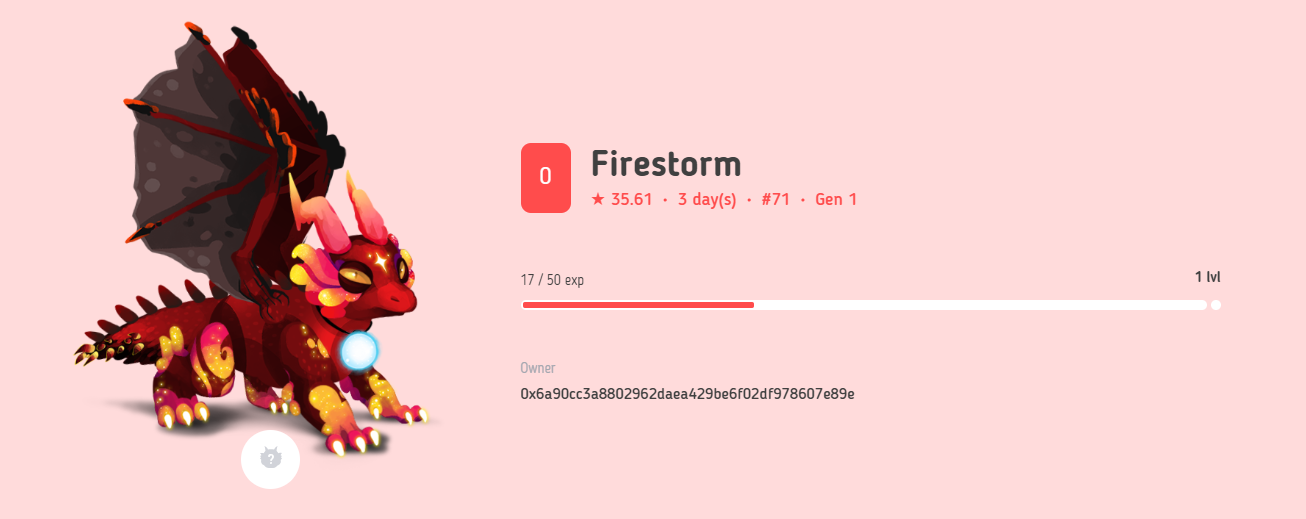
\includegraphics[width=6.27in,height=2.49in]{./media/image21.png}
		\caption{The dragon display, showing the image of the dragon, the dragon's name and the Dragon Skillfulness Index under the name.}
		\label{fig:The_dragon_display_showing_the_image_of_the_dragon_the_dragons_name_and_the_Dragon_Skillfulness_Index_on_the_left_of_the_name}
	\end{FlushLeft}\end{figure}


%%%%%%%%%%%%%%%%%%%% Figure/Image No: 5 Ends here %%%%%%%%%%%%%%%%%%%%


\par

The Dragon Skillfulness Index is calculated as follows:\par

\setlength{\parskip}{0.0pt}
\begin{center}
  \begin{equation} \label{Eq:I_{ds}}
      I_{ds}=\sum_{k=1}^{40} P_g(k),
  \end{equation}
\end{center} \par

\setlength{\parskip}{9.96pt}
Where,   $I_{ds}$ \  is the Dragon Skillfulness Index, the\ gene points,   $P_g$  are calculated in Equation   \ref{Eq:GPoints}   below, and the index k runs from 1 to 40 for each gene in the dragon’s genome as shown in Section  \ref{Blockchain breeding algorithm} . \par


\begin{center}
  \begin{equation} \label{Eq:GPoints}
     P_g=L_g*f_{gv}*f_{dr},
  \end{equation}
\end{center}
Where\   $L_g$ \ is the gene level,   $f_{gv}$  is the gene variety factor,\ and  $f_{dr}$   is the dominant or recessive factor, for a dominant gene   $f_{dr}=1$  and for a recessive gene   $f_{dr}=0.7$, described in  Section \ref{Blockchain breeding algorithm}. The gene variety factor for each dragon variety is given in  Table \ref{tab:The gene variation multiplier depending on the different dragon variations}.\par


\vspace{\baselineskip}


%%%%%%%%%%%%%%%%%%%% Table No: 5 starts here %%%%%%%%%%%%%%%%%%%%


\begin{table}[!ht]
 			\centering
\begin{tabular}{p{0.89in}p{0.79in}p{1.57in}}
\hhline{---}
%row no:1
\multicolumn{1}{|p{0.89in}|}{{\fontsize{10pt}{12.0pt}\selectfont Gene Variety}} & 
\multicolumn{1}{p{0.79in}|}{{\fontsize{10pt}{12.0pt}\selectfont Codename}} & 
\multicolumn{1}{p{1.57in}|}{\raggedleft {\fontsize{10pt}{12.0pt}\selectfont \textcolor[HTML]{333333}{Gene variety factor}}} \\
\hhline{---}
%row no:2
\multicolumn{1}{|p{0.89in}|}{{\fontsize{10pt}{12.0pt}\selectfont 1 (inbreeding)}} & 
\multicolumn{1}{p{0.79in}|}{{\fontsize{10pt}{12.0pt}\selectfont Inbreeding}} & 
\multicolumn{1}{p{1.57in}|}{\raggedleft {\fontsize{10pt}{12.0pt}\selectfont 0.5}} \\
\hhline{---}
%row no:3
\multicolumn{1}{|p{0.89in}|}{{\fontsize{10pt}{12.0pt}\selectfont 2 (regular)}} & 
\multicolumn{1}{p{0.79in}|}{{\fontsize{10pt}{12.0pt}\selectfont Common 0}} & 
\multicolumn{1}{p{1.57in}|}{\raggedleft {\fontsize{10pt}{12.0pt}\selectfont 1.2}} \\
\hhline{---}
%row no:4
\multicolumn{1}{|p{0.89in}|}{{\fontsize{10pt}{12.0pt}\selectfont 3 (regular)}} & 
\multicolumn{1}{p{0.79in}|}{{\fontsize{10pt}{12.0pt}\selectfont Common 1}} & 
\multicolumn{1}{p{1.57in}|}{\raggedleft {\fontsize{10pt}{12.0pt}\selectfont 1.2}} \\
\hhline{---}
%row no:5
\multicolumn{1}{|p{0.89in}|}{{\fontsize{10pt}{12.0pt}\selectfont 4 (regular)}} & 
\multicolumn{1}{p{0.79in}|}{{\fontsize{10pt}{12.0pt}\selectfont Common 2}} & 
\multicolumn{1}{p{1.57in}|}{\raggedleft {\fontsize{10pt}{12.0pt}\selectfont 1.2}} \\
\hhline{---}
%row no:6
\multicolumn{1}{|p{0.89in}|}{{\fontsize{10pt}{12.0pt}\selectfont 5 (regular)}} & 
\multicolumn{1}{p{0.79in}|}{{\fontsize{10pt}{12.0pt}\selectfont Common 3}} & 
\multicolumn{1}{p{1.57in}|}{\raggedleft {\fontsize{10pt}{12.0pt}\selectfont 1.2}} \\
\hhline{---}
%row no:7
\multicolumn{1}{|p{0.89in}|}{{\fontsize{10pt}{12.0pt}\selectfont 6 (regular)}} & 
\multicolumn{1}{p{0.79in}|}{{\fontsize{10pt}{12.0pt}\selectfont Rare 0}} & 
\multicolumn{1}{p{1.57in}|}{\raggedleft {\fontsize{10pt}{12.0pt}\selectfont 1.6}} \\
\hhline{---}
%row no:8
\multicolumn{1}{|p{0.89in}|}{{\fontsize{10pt}{12.0pt}\selectfont 7 (regular)}} & 
\multicolumn{1}{p{0.79in}|}{{\fontsize{10pt}{12.0pt}\selectfont Rare 1}} & 
\multicolumn{1}{p{1.57in}|}{\raggedleft {\fontsize{10pt}{12.0pt}\selectfont 1.6}} \\
\hhline{---}
%row no:9
\multicolumn{1}{|p{0.89in}|}{{\fontsize{10pt}{12.0pt}\selectfont 8 (regular)}} & 
\multicolumn{1}{p{0.79in}|}{{\fontsize{10pt}{12.0pt}\selectfont Rare 2}} & 
\multicolumn{1}{p{1.57in}|}{\raggedleft {\fontsize{10pt}{12.0pt}\selectfont 1.6}} \\
\hhline{---}
%row no:10
\multicolumn{1}{|p{0.89in}|}{{\fontsize{10pt}{12.0pt}\selectfont 9 (mystery)}} & 
\multicolumn{1}{p{0.79in}|}{{\fontsize{10pt}{12.0pt}\selectfont Epic 0}} & 
\multicolumn{1}{p{1.57in}|}{\raggedleft {\fontsize{10pt}{12.0pt}\selectfont 2.8}} \\
\hhline{---}
%row no:11
\multicolumn{1}{|p{0.89in}|}{{\fontsize{10pt}{12.0pt}\selectfont 10 (mystery)}} & 
\multicolumn{1}{p{0.79in}|}{{\fontsize{10pt}{12.0pt}\selectfont Epic 1}} & 
\multicolumn{1}{p{1.57in}|}{\raggedleft {\fontsize{10pt}{12.0pt}\selectfont 2.8}} \\
\hhline{---}

\end{tabular}\caption{The gene variation multiplier depending on the different dragon variations}
\label{tab:The gene variation multiplier depending on the different dragon variations}

\end{table}


%%%%%%%%%%%%%%%%%%%% Table No: 5 ends here %%%%%%%%%%%%%%%%%%%%


\subsection{Special attack and special defense skills}
%\addcontentsline{toc}{subsection}{Special attack and special defense skills}
\label{Special attack and special defense skills}  \par

\textit{Special attack} or \textit{special defense} is the ability to use the special powers available to each dragon family. It improves the \textit{attack} or \textit{defense} during a battle move. Those special skills use Mana. In  Table \ref{tab:Table of Mana costs, multipliers for a attack/defense and a probability of activation for Special Attack and Special Defense.} the amount of Mana necessary for the activation of the \textit{special attack }or the \textit{special defense }skill depending on the type of dragon is shown as well as the probability for its activation.\par

For dragons with a mixed genome as a result of the breeding process the type used for special skills is determined during the incubation process by a factored random and stored in the type field in the specialAttacks/specialDefenses mappings (see Section \ref{Blockchain breeding algorithm}).\par


%%%%%%%%%%%%%%%%%%%% Table No: 6 starts here %%%%%%%%%%%%%%%%%%%%


\begin{table}[!ht]
 			\centering
\begin{tabular}{p{1.48in}p{0.88in}p{0.88in}p{0.88in}p{0.88in}p{0.88in}}
\hhline{------}
%row no:1
\multicolumn{1}{|p{1.48in}|}{{\fontsize{10pt}{12.0pt}\selectfont Dragon type}} & 
\multicolumn{1}{p{0.78in}|}{\centering{\fontsize{10pt}{12.0pt}\selectfont Fire}} & 
\multicolumn{1}{p{0.78in}|}{\centering{\fontsize{10pt}{12.0pt}\selectfont Water}} & 
\multicolumn{1}{p{0.78in}|}{\centering{\fontsize{10pt}{12.0pt}\selectfont Earth}} & 
\multicolumn{1}{p{0.78in}|}{\centering{\fontsize{10pt}{12.0pt}\selectfont Air}} & 
\multicolumn{1}{p{0.78in}|}{\centering{\fontsize{10pt}{12.0pt}\selectfont Cyber}} \\
\hhline{------}
%row no:2
\multicolumn{6}{|p{5.58in}|}{\Centering {\fontsize{10pt}{12.0pt}\selectfont Special Attack skills details}} \\
\hhline{------}
%row no:3
\multicolumn{1}{|p{1.48in}|}{{\fontsize{10pt}{12.0pt}\selectfont Mana points}} & 
\multicolumn{1}{p{0.78in}|}{\centering{{\fontsize{10pt}{12.0pt}\selectfont   $3 \times A $ }}} & 
\multicolumn{1}{p{0.78in}|}{\centering{{\fontsize{10pt}{12.0pt}\selectfont   $3 \times S $ }}} & 
\multicolumn{1}{p{0.78in}|}{\centering{{\fontsize{10pt}{12.0pt}\selectfont   $3 \times D $ }}} & 
\multicolumn{1}{p{0.78in}|}{\centering{{\fontsize{10pt}{12.0pt}\selectfont   $3 \times V $ }}} & 
\multicolumn{1}{p{0.78in}|}{\centering{{\fontsize{10pt}{12.0pt}\selectfont   $3 \times I $ }}} \\
\hhline{------}
%row no:4
\multicolumn{1}{|p{1.48in}|}{{\fontsize{10pt}{12.0pt}\selectfont Attack factor}} & 
\multicolumn{1}{p{0.78in}|}{\centering{{\fontsize{10pt}{12.0pt}\selectfont   $\sqrt{A/3}+1$}}} & 
\multicolumn{1}{p{0.78in}|}{\centering{{\fontsize{10pt}{12.0pt}\selectfont   $\sqrt{S/3}+1$}}} & 
\multicolumn{1}{p{0.78in}|}{\centering{{\fontsize{10pt}{12.0pt}\selectfont   $\sqrt{D/3}+1$}}} & 
\multicolumn{1}{p{0.78in}|}{\centering{{\fontsize{10pt}{12.0pt}\selectfont   $\sqrt{V/3}+1$}}} & 
\multicolumn{1}{p{0.78in}|}{\centering{{\fontsize{10pt}{12.0pt}\selectfont   $\sqrt{I/3}+1$}}} \\
\hhline{------}
%row no:5
\multicolumn{1}{|p{1.48in}|}{{\fontsize{10pt}{12.0pt}\selectfont Probability\hspace{0.1cm}of  activation}} & 
\multicolumn{1}{p{0.78in}|}{\centering{{\fontsize{10pt}{12.0pt}\selectfont   $\sqrt I+10$}}} & 
\multicolumn{1}{p{0.78in}|}{\centering{{\fontsize{10pt}{12.0pt}\selectfont   $\sqrt I+10$}}} & 
\multicolumn{1}{p{0.78in}|}{\centering{{\fontsize{10pt}{12.0pt}\selectfont   $\sqrt I+10$}}} & 
\multicolumn{1}{p{0.78in}|}{\centering{{\fontsize{10pt}{12.0pt}\selectfont   $\sqrt I+10$}}} & 
\multicolumn{1}{p{0.78in}|}{\centering{{\fontsize{10pt}{12.0pt}\selectfont   $\sqrt I+10$}}} \\
\hhline{------}
%row no:6
\multicolumn{6}{|p{5.58in}|}{\Centering {\fontsize{10pt}{12.0pt}\selectfont Special Defense skills details}} \\
\hhline{------}
%row no:7
\multicolumn{1}{|p{1.48in}|}{{\fontsize{10pt}{12.0pt}\selectfont Mana points}} & 
\multicolumn{1}{p{0.78in}|}{\centering{{\fontsize{10pt}{12.0pt}\selectfont   $3 \times A $ }}} & 
\multicolumn{1}{p{0.78in}|}{\centering{{\fontsize{10pt}{12.0pt}\selectfont   $3 \times S $ }}} & 
\multicolumn{1}{p{0.78in}|}{\centering{{\fontsize{10pt}{12.0pt}\selectfont   $3 \times D $ }}} & 
\multicolumn{1}{p{0.78in}|}{\centering{{\fontsize{10pt}{12.0pt}\selectfont   $3 \times V $ }}} & 
\multicolumn{1}{p{0.78in}|}{\centering{{\fontsize{10pt}{12.0pt}\selectfont   $3 \times I $ }}} \\
\hhline{------}
%row no:8
\multicolumn{1}{|p{1.48in}|}{{\fontsize{10pt}{12.0pt}\selectfont Defense factor}} & 
\multicolumn{1}{p{0.78in}|}{\centering{{\fontsize{10pt}{12.0pt}\selectfont   $\sqrt{A/3}+1$ }}} & 
\multicolumn{1}{p{0.78in}|}{\centering{{\fontsize{10pt}{12.0pt}\selectfont   $\sqrt{S/3}+1$ }}} & 
\multicolumn{1}{p{0.78in}|}{\centering{{\fontsize{10pt}{12.0pt}\selectfont   $\sqrt{D/3}+1$ }}} & 
\multicolumn{1}{p{0.78in}|}{\centering{{\fontsize{10pt}{12.0pt}\selectfont   $\sqrt{V/3}+1$ }}} & 
\multicolumn{1}{p{0.78in}|}{\centering{{\fontsize{10pt}{12.0pt}\selectfont   $\sqrt{I/3}+1$ }}} \\
\hhline{------}
%row no:9
\multicolumn{1}{|p{1.48in}|}{{\fontsize{10pt}{12.0pt}\selectfont Probability\hspace{0.1cm}of activation}} & 
\multicolumn{1}{p{0.78in}|}{\centering{{\fontsize{10pt}{12.0pt}\selectfont   $\sqrt I+10$}}} & 
\multicolumn{1}{p{0.78in}|}{\centering{{\fontsize{10pt}{12.0pt}\selectfont   $\sqrt I+10$}}} & 
\multicolumn{1}{p{0.78in}|}{\centering{{\fontsize{10pt}{12.0pt}\selectfont   $\sqrt I+10$}}} & 
\multicolumn{1}{p{0.78in}|}{\centering{{\fontsize{10pt}{12.0pt}\selectfont   $\sqrt I+10$}}} & 
\multicolumn{1}{p{0.78in}|}{\centering{{\fontsize{10pt}{12.0pt}\selectfont   $\sqrt I+10$}}} \\
\hhline{------}

\end{tabular}\caption{Table of Mana costs, multipliers for a attack/defense and a probability of activation for Special Attack and Special Defense.}
\label{tab:Table of Mana costs, multipliers for a attack/defense and a probability of activation for Special Attack and Special Defense.}

 \end{table}


%%%%%%%%%%%%%%%%%%%% Table No: 6 ends here %%%%%%%%%%%%%%%%%%%%


\subsection{Special peaceful skills}
%\addcontentsline{toc}{subsection}{Special peaceful skills}
\label{Special peaceful skills}  \par

The maximum Level Up for a dragon is 10. On the 10th Level Up, the player can obtain a \textit{special peaceful skills} for their dragon.\par

A \textit{special peaceful skill} allows users to earn in-game currency in exchange for offering skills to the game community on the game’s marketplace\footnote{The price of the {\it special peaceful skills}, alongside the prices of other items, such as dragons and eggs, traded on the marketplace will be decided by the market forces. The role of Dragonereum will only be to provide the internal marketplace to facilitate trade, however players will be able to interact directly with smart contracts and third-party marketplaces can be introduced.}.\par

A dragon can buy a \textit{special peaceful skill} that can be used in order to receive a boost to one of its \textit{basic skills as }shown in the first five rows of  Table \ref{tab:Table showing the different special skills that can be obtained (column 1), the Mana points the selling dragon needs to offer each skill (column 2) and the factor showing the increase in skill (column3).}. After the boost has been applied, the \textit{basic skill }defined in Equation \ref{Eq:Sk} will become $Sk^{new}(j)=f_j\times Sk^{old}(j)$, with $f_j$ being the Action Factor and j denoting the basic skill, $j \in$  {A (attack), D (defense), S (stamina), V (speed), I (intelligence)}.This boost will be available to use for only one battle, thus incentivizing players to find an opponent and commence a battle as soon as they have bought the \textit{special peaceful skill }and applied the boost to one of their \textit{basic skills}. Alternatively, a player can buy a \textit{special peaceful skill}, which will recharge the Health or Mana points of the dragon, bottom two rows of  Table \ref{tab:Table showing the different special skills that can be obtained (column 1), the Mana points the selling dragon needs to offer each skill (column 2) and the factor showing the increase in skill (column3).}.\par

The dragon offering the \textit{special peaceful skill} will have to use its Mana points to be able to offer the service. The amount of Mana points necessary for each different \textit{special peaceful skill} is shown in column 2 of  Table \ref{tab:Table showing the different special skills that can be obtained (column 1), the Mana points the selling dragon needs to offer each skill (column 2) and the factor showing the increase in skill (column3).}. The selling dragon will receive the in-game currency reward for the service it provided, and its Mana points will restore themselves over time.\par



%%%%%%%%%%%%%%%%%%%% Table No: 7 starts here %%%%%%%%%%%%%%%%%%%%


\begin{table}[H]
 			\centering
\begin{tabular}{p{1.49in}p{1.92in}p{2.62in}}
\hhline{---}
%row no:1
\multicolumn{1}{|p{1.49in}|}{{\fontsize{10pt}{12.0pt}\selectfont Special peaceful skill}} & 
\multicolumn{1}{p{1.92in}|}{{\fontsize{10pt}{12.0pt}\selectfont Action Factor}} & 
\multicolumn{1}{p{2.62in}|}{{\fontsize{10pt}{12.0pt}\selectfont Mana points }} \\
\hhline{---}
%row no:2
\multicolumn{1}{|p{1.49in}|}{{\fontsize{10pt}{12.0pt}\selectfont Attack boost}} & 
\multicolumn{1}{p{1.92in}|}{$f_A=\sqrt{A/30}+1$} & 
\multicolumn{1}{p{2.62in}|}{ $3\times A$ } \\
\hhline{---}
%row no:3
\multicolumn{1}{|p{1.49in}|}{{\fontsize{10pt}{12.0pt}\selectfont Stamina boost}} & 
\multicolumn{1}{p{1.92in}|}{$f_S=\sqrt{S/30}+1$} & 
\multicolumn{1}{p{2.62in}|}{ $3\times S${\fontsize{10pt}{12.0pt}\selectfont  }} \\
\hhline{---}
%row no:4
\multicolumn{1}{|p{1.49in}|}{{\fontsize{10pt}{12.0pt}\selectfont Defense boost}} & 
\multicolumn{1}{p{1.92in}|}{$f_D=\sqrt{D/30}+1$} & 
\multicolumn{1}{p{2.62in}|}{ $3\times D${\fontsize{10pt}{12.0pt}\selectfont  }} \\
\hhline{---}
%row no:5
\multicolumn{1}{|p{1.49in}|}{{\fontsize{10pt}{12.0pt}\selectfont Speed boost}} & 
\multicolumn{1}{p{1.92in}|}{$f_V=\sqrt{V/30}+1$} & 
\multicolumn{1}{p{2.62in}|}{ $3\times V${\fontsize{10pt}{12.0pt}\selectfont  }} \\
\hhline{---}
%row no:6
\multicolumn{1}{|p{1.49in}|}{{\fontsize{10pt}{12.0pt}\selectfont Intelligence boost}} & 
\multicolumn{1}{p{1.92in}|}{$f_I=\sqrt{I/30}+1$} & 
\multicolumn{1}{p{2.62in}|}{ $3\times I${\fontsize{10pt}{12.0pt}\selectfont  }} \\
\hhline{---}
%row no:7
\multicolumn{1}{|p{1.49in}|}{{\fontsize{10pt}{12.0pt}\selectfont Healing}} & 
\multicolumn{1}{p{1.92in}|}{$H_R=2 \times S$} & 
\multicolumn{1}{p{2.62in}|}{ $3\times S$ } \\
\hhline{---}
%row no:8
\multicolumn{1}{|p{1.49in}|}{{\fontsize{10pt}{12.0pt}\selectfont Mana recharge}} & 
\multicolumn{1}{p{1.92in}|}{$M_R=2 \times I$} & 
\multicolumn{1}{p{2.62in}|}{ $3\times I$ } \\
\hhline{---}

\end{tabular}\caption{Table showing the different special skills that can be obtained (column 1), the Mana points the selling dragon needs to offer each skill (column 2) and the factor showing the increase in skill (column3).}
\label{tab:Table showing the different special skills that can be obtained (column 1), the Mana points the selling dragon needs to offer each skill (column 2) and the factor showing the increase in skill (column3).}

 \end{table}


%%%%%%%%%%%%%%%%%%%% Table No: 7 ends here %%%%%%%%%%%%%%%%%%%%
\textit{Special peaceful skills} can be used in both regular and gladiator battles. In the case of gladiator battles a dragon will be freezed once the battle is initiated and no \textit{special  peaceful skill} or body part level ups can be applied.\par

\setlength{\parskip}{9.96pt}
\subsection{Leveling up dragons}
%\addcontentsline{toc}{subsection}{Leveling up dragons}
 \label{Leveling up dragons}   \par

A dragon will be able to breed only if it has accumulated the required number of XP for a Dragon Level Up and as a result has acquired the necessary amount of DP.\par

At this point, a user will have to decide whether to upgrade their dragon (level up its body parts and get a stronger dragon) or to interbreed it with another dragon.\par

Additionally, getting dragon offsprings will become more and more difficult when going up levels as the required amount of XP will increase from level to level. Therefore, it will be necessary to have, and to win more and more battles.\par
\begin{Center}
%%%%%%%%%%%%%%%%%%%% Figure/Image No: 6 starts here %%%%%%%%%%%%%%%%%%%%
\begin{figure}[!ht]
	\begin{Center}
		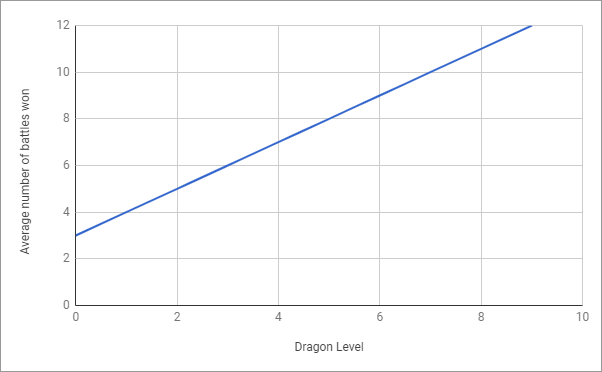
\includegraphics[width=6.09in,height=3.77in]{./media/image17.png}
		\caption{Average number of battles won required for a dragon Level Up}
		\label{fig:Average_number_of_battles_won_required_for_a_dragon_Level_Up}
	\end{Center}
\end{figure}
%%%%%%%%%%%%%%%%%%%% Figure/Image No: 6 Ends here %%%%%%%%%%%%%%%%%%%%
\end{Center}
Before we describe the growing difficulty in acquiring DP we have to look at how the DS is calculated,\par
\begin{center}
  \begin{equation} \label{Eq:DS}
    DS=0.7*A+2.1*D+2.3*S+1.1*V+1.5*I,
  \end{equation}
\end{center}
where A is the \textit{attack}, D is the \textit{defense}, S is the \textit{stamina}, V is the \textit{speed}, and I the \textit{intelligence} of the dragon. The \textit{basic skills} are calculated in Equation \ref{Eq:Sk}\footnote{In the equation $Sk(attack)\equiv A$, $Sk(defense)\equiv D$, $Sk(stamina)\equiv S$, $Sk(speed)\equiv V$, $Sk(intelligence)\equiv I$}.  \par

The constants in Equation \ref{Eq:DS} were carefully obtained through a rigorous simulation procedure ensuring that dragons with similar DS have an equal chance at winning the battle. Numerous battles between randomly chosen dragons with a similar amount of total basic skills were simulated and if there were battles where a dragon had an advantage, the values were adjusted in order to avoid this situation. The process was repeated until there were no dragons that had a winning advantage and every dragon, regardless of their skills or traits, has a 50$\%$  chance of winning against a dragon with a similar DS.\par

Based on the DS, the game’s algorithms offer suitable opponents for regular battles. A short description and the corresponding code for the regular battles are given in the Appendix.\par

As a result of these battles the winners will receive XP. The number of XP won, in the case when the attacking dragon is the winner, is calculated according to the formulas below.\par


\begin{center}
  \begin{equation}
    XP_e= \begin{cases}
    \left(\frac{DS_{d}}{DS_{w}}\right)^5 & \mbox{if } DS_{d} < DS_{w}\\
    \left(\frac{DS_{d}}{DS_{w}}\right)^2 & \mbox{if } DS_{d} \geq DS_{w},
    \end{cases}
  \end{equation}
\end{center}

\vspace{\baselineskip}
where $XP_e$ are the Experience Points earned after a battle, $DS_{d}$\ \  is the DS of the defeated dragon, and $DS_{w}$ is the DS of the winning dragon. In the case when the attacking dragon loses, and the defending dragon wins, XP won is calculated according to the formulas below, however it is limited by the algorithm to be not more than 10.\par 

\begin{center}
	\begin{equation}
	XP_e= \begin{cases}
	\left(\frac{DS_{d}}{DS_{w}}\right)^5/2 & \mbox{if } DS_{d} < DS_{w}\\
	\left(\frac{DS_{d}}{DS_{w}}\right)/2 & \mbox{if } DS_{d} \geq DS_{w},
	\end{cases}
	\end{equation}
\end{center}

The reduction in the number of XP won is done in order to incentivize the attacking dragons, which use gas to initiate the transaction on Ethereum.\par

Once the required amount of XP is accumulated the dragon will get a dragon level up. There are ten Dragon Level Ups possible for each dragon. Each next dragon level up requires more XP and therefore more battles to be won, see  Table \ref{tab:The amount of XP required for a level up at each level (0-10).}.\par

At the same time the strongest dragon in the population will likely get less XP as a result of battles as it will become more and more difficult to find an opponent of the same or higher DS, thereby limiting the number of battles it can have\textit{ }on the one hand and minimizing the amount of XP it can obtain by winning battles on the other.\par




%%%%%%%%%%%%%%%%%%%% Table No: 8 starts here %%%%%%%%%%%%%%%%%%%%


\begin{table}[!ht]
 			\centering
\begin{tabular}{p{0.84in}p{2.61in}}
\hhline{--}
%row no:1
\multicolumn{1}{|p{0.84in}|}{{\fontsize{10pt}{12.0pt}\selectfont Dragon Level}} & 
\multicolumn{1}{p{2.61in}|}{{\fontsize{10pt}{12.0pt}\selectfont Experience Points required for a level up}} \\
\hhline{--}
%row no:2
\multicolumn{1}{|p{0.84in}|}{\raggedleft {\fontsize{10pt}{12.0pt}\selectfont 0}} & 
\multicolumn{1}{p{2.61in}|}{\raggedleft {\fontsize{10pt}{12.0pt}\selectfont 30}} \\
\hhline{--}
%row no:3
\multicolumn{1}{|p{0.84in}|}{\raggedleft {\fontsize{10pt}{12.0pt}\selectfont 1}} & 
\multicolumn{1}{p{2.61in}|}{\raggedleft {\fontsize{10pt}{12.0pt}\selectfont 40}} \\
\hhline{--}
%row no:4
\multicolumn{1}{|p{0.84in}|}{\raggedleft {\fontsize{10pt}{12.0pt}\selectfont 2}} & 
\multicolumn{1}{p{2.61in}|}{\raggedleft {\fontsize{10pt}{12.0pt}\selectfont 50}} \\
\hhline{--}
%row no:5
\multicolumn{1}{|p{0.84in}|}{\raggedleft {\fontsize{10pt}{12.0pt}\selectfont 3}} & 
\multicolumn{1}{p{2.61in}|}{\raggedleft {\fontsize{10pt}{12.0pt}\selectfont 60}} \\
\hhline{--}
%row no:6
\multicolumn{1}{|p{0.84in}|}{\raggedleft {\fontsize{10pt}{12.0pt}\selectfont 4}} & 
\multicolumn{1}{p{2.61in}|}{\raggedleft {\fontsize{10pt}{12.0pt}\selectfont 70}} \\
\hhline{--}
%row no:7
\multicolumn{1}{|p{0.84in}|}{\raggedleft {\fontsize{10pt}{12.0pt}\selectfont 5}} & 
\multicolumn{1}{p{2.61in}|}{\raggedleft {\fontsize{10pt}{12.0pt}\selectfont 80}} \\
\hhline{--}
%row no:8
\multicolumn{1}{|p{0.84in}|}{\raggedleft {\fontsize{10pt}{12.0pt}\selectfont 6}} & 
\multicolumn{1}{p{2.61in}|}{\raggedleft {\fontsize{10pt}{12.0pt}\selectfont 90}} \\
\hhline{--}
%row no:9
\multicolumn{1}{|p{0.84in}|}{\raggedleft {\fontsize{10pt}{12.0pt}\selectfont 7}} & 
\multicolumn{1}{p{2.61in}|}{\raggedleft {\fontsize{10pt}{12.0pt}\selectfont 100}} \\
\hhline{--}
%row no:10
\multicolumn{1}{|p{0.84in}|}{\raggedleft {\fontsize{10pt}{12.0pt}\selectfont 8}} & 
\multicolumn{1}{p{2.61in}|}{\raggedleft {\fontsize{10pt}{12.0pt}\selectfont 110}} \\
\hhline{--}
%row no:11
\multicolumn{1}{|p{0.84in}|}{\raggedleft {\fontsize{10pt}{12.0pt}\selectfont 9}} & 
\multicolumn{1}{p{2.61in}|}{\raggedleft {\fontsize{10pt}{12.0pt}\selectfont 120}} \\
\hhline{--}
%row no:12
\multicolumn{1}{|p{0.84in}|}{\raggedleft {\fontsize{10pt}{12.0pt}\selectfont 10}} & 
\multicolumn{1}{p{2.61in}|}{\raggedleft {\fontsize{10pt}{12.0pt}\selectfont -}} \\
\hhline{--}

\end{tabular}\caption{The amount of XP required for a level up at each level (0-10).}
\label{tab:The amount of XP required for a level up at each level (0-10).}

 \end{table}


%%%%%%%%%%%%%%%%%%%% Table No: 8 ends here %%%%%%%%%%%%%%%%%%%%

Once a dragon goes up a level it receives DNA Points which are allocated according to  Table \ref{tab:Number of AP received after leveling up at each level  (0-10).} below.\par

%%%%%%%%%%%%%%%%%%%% Table No: 9 starts here %%%%%%%%%%%%%%%%%%%%


\begin{table}[!ht]
 			\centering
\begin{tabular}{p{0.84in}p{2.58in}}
\hhline{--}
%row no:1
\multicolumn{1}{|p{0.84in}|}{{\fontsize{10pt}{12.0pt}\selectfont Dragon Level}} & 
\multicolumn{1}{p{2.58in}|}{{\fontsize{10pt}{12.0pt}\selectfont DNA Points received after leveling up}} \\
\hhline{--}
%row no:2
\multicolumn{1}{|p{0.84in}|}{\raggedleft {\fontsize{10pt}{12.0pt}\selectfont 0}} & 
\multicolumn{1}{p{2.58in}|}{\raggedleft {\fontsize{10pt}{12.0pt}\selectfont 0}} \\
\hhline{--}
%row no:3
\multicolumn{1}{|p{0.84in}|}{\raggedleft {\fontsize{10pt}{12.0pt}\selectfont 1}} & 
\multicolumn{1}{p{2.58in}|}{\raggedleft {\fontsize{10pt}{12.0pt}\selectfont 10}} \\
\hhline{--}
%row no:4
\multicolumn{1}{|p{0.84in}|}{\raggedleft {\fontsize{10pt}{12.0pt}\selectfont 2}} & 
\multicolumn{1}{p{2.58in}|}{\raggedleft {\fontsize{10pt}{12.0pt}\selectfont 13}} \\
\hhline{--}
%row no:5
\multicolumn{1}{|p{0.84in}|}{\raggedleft {\fontsize{10pt}{12.0pt}\selectfont 3}} & 
\multicolumn{1}{p{2.58in}|}{\raggedleft {\fontsize{10pt}{12.0pt}\selectfont 16}} \\
\hhline{--}
%row no:6
\multicolumn{1}{|p{0.84in}|}{\raggedleft {\fontsize{10pt}{12.0pt}\selectfont 4}} & 
\multicolumn{1}{p{2.58in}|}{\raggedleft {\fontsize{10pt}{12.0pt}\selectfont 21}} \\
\hhline{--}
%row no:7
\multicolumn{1}{|p{0.84in}|}{\raggedleft {\fontsize{10pt}{12.0pt}\selectfont 5}} & 
\multicolumn{1}{p{2.58in}|}{\raggedleft {\fontsize{10pt}{12.0pt}\selectfont 28}} \\
\hhline{--}
%row no:8
\multicolumn{1}{|p{0.84in}|}{\raggedleft {\fontsize{10pt}{12.0pt}\selectfont 6}} & 
\multicolumn{1}{p{2.58in}|}{\raggedleft {\fontsize{10pt}{12.0pt}\selectfont 37}} \\
\hhline{--}
%row no:9
\multicolumn{1}{|p{0.84in}|}{\raggedleft {\fontsize{10pt}{12.0pt}\selectfont 7}} & 
\multicolumn{1}{p{2.58in}|}{\raggedleft {\fontsize{10pt}{12.0pt}\selectfont 48}} \\
\hhline{--}
%row no:10
\multicolumn{1}{|p{0.84in}|}{\raggedleft {\fontsize{10pt}{12.0pt}\selectfont 8}} & 
\multicolumn{1}{p{2.58in}|}{\raggedleft {\fontsize{10pt}{12.0pt}\selectfont 62}} \\
\hhline{--}
%row no:11
\multicolumn{1}{|p{0.84in}|}{\raggedleft {\fontsize{10pt}{12.0pt}\selectfont 9}} & 
\multicolumn{1}{p{2.58in}|}{\raggedleft {\fontsize{10pt}{12.0pt}\selectfont 81}} \\
\hhline{--}
%row no:12
\multicolumn{1}{|p{0.84in}|}{\raggedleft {\fontsize{10pt}{12.0pt}\selectfont 10}} & 
\multicolumn{1}{p{2.58in}|}{\raggedleft {\fontsize{10pt}{12.0pt}\selectfont 106}} \\
\hhline{--}

\end{tabular}\caption{The amount of DP received after leveling up at each level  (0-10).}
\label{tab:Number of AP received after leveling up at each level  (0-10).}

 \end{table}


%%%%%%%%%%%%%%%%%%%% Table No: 9 ends here %%%%%%%%%%%%%%%%%%%%
\begin{samepage}
DP might be spent on:
  \begin{itemize}
	\item body parts level up\par

	\item breeding\par
  \end{itemize}
\end{samepage}

Body part level ups will increase the total \textit{basic skills} as is shown in  Equation \ref{Eq:Sk},\  since every body part level up gives a boost to the corresponding skills it is responsible for (see Table \ref{tab:The table shows which body parts are responsible for which particular skills.})\footnote{When the body part level up increases the active gene’s level for that body part increases as well, since they are identical, however the levels of the other three genes in the body part set remain the same. From this arises the possibility that a dragon’s offspring will inherit one of these three genes as its active gene and will have lower initial basic skills than its parents.}. The example of how this is calculated is given in  Table \ref{tab:An example, illustrating the calculation of the basic skill for a specific body part - the Ashed Legs at level 3 of a particular dragon.} in Section  \ref{Calculating the overall basic skills of a dragon}.\par

The amount of DP required for a body part level up is calculated as follows:
\begin{center}
   \begin{equation} \label{Eq:CAP}
     C_{DP}(L_n) = Round(1.02 \times C_{DP}(L_{n-1})),
   \end{equation}
\end{center}
where\ \  $C_{DP}(L_n)$\ is the cost of the body part level up at level  $L_n$  and $C_{DP}(L_{n-1})$\ is the cost of the body part level up at level  $L_{n-1}$  correspondingly. The expression on the right hand side of the equation is rounded to the nearest hundredth, and this value is then used for the calculation of the cost at the next level and so on (the actual DP points are further rounded to the nearest integer). \ The first term in the series is  $C_{DP}(L_0)=10$, so 10 dP are required to level up a body part to level 1.  The DP points required for leveling up a body part, calculated in Equation \ref{Eq:CAP} are presented in Figure  \ref{fig:The_amount_of_Action_Points_necessary_for_a_body_part_level_up_at_each_level_099} as a function of the body part level.\par
\begin{Center}


%%%%%%%%%%%%%%%%%%%% Figure/Image No: 7 starts here %%%%%%%%%%%%%%%%%%%%

\begin{figure}[!ht]
	\begin{Center}
		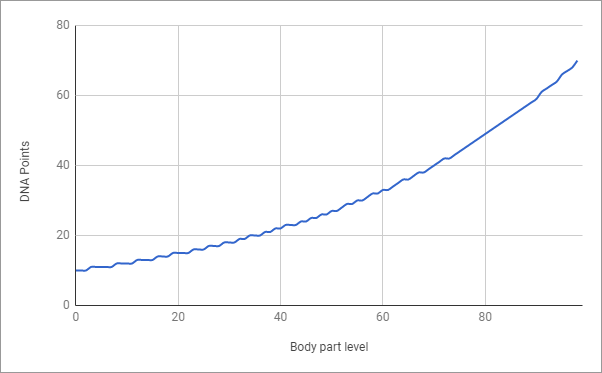
\includegraphics[width=6.27in,height=3.89in]{./media/image20.png}
		\caption{The amount of DNA Points necessary for a body part level up at each level (0-99)}
		\label{fig:The_amount_of_Action_Points_necessary_for_a_body_part_level_up_at_each_level_099}
	\end{Center}
\end{figure}


%%%%%%%%%%%%%%%%%%%% Figure/Image No: 7 Ends here %%%%%%%%%%%%%%%%%%%%



\end{Center}
Here we will look at the amount of DNA Points required for breeding at each level, see  Table \ref{tab:The amount of AP required for breeding at each level (0-10).}.\par


%%%%%%%%%%%%%%%%%%%% Table No: 10 starts here %%%%%%%%%%%%%%%%%%%%


\begin{table}[!ht]
 			\centering
\begin{tabular}{p{0.81in}p{2.59in}}
\hhline{--}
%row no:1
\multicolumn{1}{|p{0.81in}|}{{\fontsize{10pt}{12.0pt}\selectfont Dragon Level}} & 
\multicolumn{1}{p{2.59in}|}{{\fontsize{10pt}{12.0pt}\selectfont DNA Points required for breeding}} \\
\hhline{--}
%row no:2
\multicolumn{1}{|p{0.84in}|}{\raggedleft {\fontsize{10pt}{12.0pt}\selectfont 0}} & 
\multicolumn{1}{p{2.58in}|}{\raggedleft {\fontsize{10pt}{12.0pt}\selectfont -}} \\
\hhline{--}
%row no:3
\multicolumn{1}{|p{0.84in}|}{\raggedleft {\fontsize{10pt}{12.0pt}\selectfont 1}} & 
\multicolumn{1}{p{2.58in}|}{\raggedleft {\fontsize{10pt}{12.0pt}\selectfont 10}} \\
\hhline{--}
%row no:4
\multicolumn{1}{|p{0.84in}|}{\raggedleft {\fontsize{10pt}{12.0pt}\selectfont 2}} & 
\multicolumn{1}{p{2.58in}|}{\raggedleft {\fontsize{10pt}{12.0pt}\selectfont 13}} \\
\hhline{--}
%row no:5
\multicolumn{1}{|p{0.84in}|}{\raggedleft {\fontsize{10pt}{12.0pt}\selectfont 3}} & 
\multicolumn{1}{p{2.58in}|}{\raggedleft {\fontsize{10pt}{12.0pt}\selectfont 16}} \\
\hhline{--}
%row no:6
\multicolumn{1}{|p{0.84in}|}{\raggedleft {\fontsize{10pt}{12.0pt}\selectfont 4}} & 
\multicolumn{1}{p{2.58in}|}{\raggedleft {\fontsize{10pt}{12.0pt}\selectfont 21}} \\
\hhline{--}
%row no:7
\multicolumn{1}{|p{0.84in}|}{\raggedleft {\fontsize{10pt}{12.0pt}\selectfont 5}} & 
\multicolumn{1}{p{2.58in}|}{\raggedleft {\fontsize{10pt}{12.0pt}\selectfont 28}} \\
\hhline{--}
%row no:8
\multicolumn{1}{|p{0.84in}|}{\raggedleft {\fontsize{10pt}{12.0pt}\selectfont 6}} & 
\multicolumn{1}{p{2.58in}|}{\raggedleft {\fontsize{10pt}{12.0pt}\selectfont 37}} \\
\hhline{--}
%row no:9
\multicolumn{1}{|p{0.84in}|}{\raggedleft {\fontsize{10pt}{12.0pt}\selectfont 7}} & 
\multicolumn{1}{p{2.58in}|}{\raggedleft {\fontsize{10pt}{12.0pt}\selectfont 48}} \\
\hhline{--}
%row no:10
\multicolumn{1}{|p{0.84in}|}{\raggedleft {\fontsize{10pt}{12.0pt}\selectfont 8}} & 
\multicolumn{1}{p{2.58in}|}{\raggedleft {\fontsize{10pt}{12.0pt}\selectfont 62}} \\
\hhline{--}
%row no:11
\multicolumn{1}{|p{0.84in}|}{\raggedleft {\fontsize{10pt}{12.0pt}\selectfont 9}} & 
\multicolumn{1}{p{2.58in}|}{\raggedleft {\fontsize{10pt}{12.0pt}\selectfont 81}} \\
\hhline{--}
%row no:12
\multicolumn{1}{|p{0.84in}|}{\raggedleft {\fontsize{10pt}{12.0pt}\selectfont 10}} & 
\multicolumn{1}{p{2.58in}|}{\raggedleft {\fontsize{10pt}{12.0pt}\selectfont 106}} \\
\hhline{--}

\end{tabular}\caption{The amount of DP required for breeding at each level (0-10).}
\label{tab:The amount of AP required for breeding at each level (0-10).}

 \end{table}

%%%%%%%%%%%%%%%%%%%% Table No: 10 ends here %%%%%%%%%%%%%%%%%%%%


\setlength{\parskip}{9.96pt}
As can be noted, the amount of DP received (see  Table \ref{tab:Number of AP received after leveling up at each level  (0-10).}) and the amount of DP required for breeding (see Table \ref{tab:The amount of AP required for breeding at each level (0-10).}) are the same at each level. Therefore, a dragon has a choice between two options, it can either breed or upgrade its skills. The system will favor the spending of DP on breeding while on the same level where those DP were received, as once a dragon moves to the next level this amount of DP will only be sufficient for a body part level up.\par

\subsection{Early adopter advantage}
%\addcontentsline{toc}{subsection}{Early adopter advantage}
\label{Early adopter advantage} \par

As\ it was discussed in  Section \ref{Introduction to Dragonereum}  the game has the Treasury, where all unallocated Gold is held. It is used to reward battle winners and leaderboard entrants. The \textit{battle winner reward} is calculated using Equation \ref{Eq:R}  below,\par


\begin{center}
  \begin{equation}\label{Eq:R}
    R=\left(\frac{G}{N_d^2}\right)*I_{ds}*10*f_{DS},
  \end{equation}
\end{center}

\vspace{\baselineskip}
\textit{w}here R is the \textit{battle winner reward}, G is the Gold balance in the Treasury, $I_{ds}$ was defined in Equation \ref{Eq:I_{ds}} above, and $f_{DS}$ is the \textit{dragon strength} \textit{factor} defined as,\par


\begin{center}
  \begin{equation}
   f_{DS}=\begin{cases}
     \left(\frac{DS_{d}}{DS_{w}}\right)^8 & \mbox{if }  DS_{d} < DS_{w}\\
     \\
     \frac{DS_{d}}{DS_{w}} & \mbox{if } DS_{d}>DS_{w}.\\
    \end{cases}
  \end{equation}
\end{center}

\vspace{\baselineskip}
However, R, is subject to the following rules:\par

\begin{itemize}
  \begin{samepage}
	\item If there are less than 15000 dragons in the population the maximum \textit{battle winner reward} is 200 Gold coins;\par

	\item If there is more than 15000 but less than 30000 dragons in the population, the maximum \textit{battle winner reward} is 100 Gold coins;\par

	\item Else (more than 30000 dragons) the maximum \textit{battle winner reward} is 25 Gold coins.
  \end{samepage}
\end{itemize}\par

Additionally, due to the early adopter advantage, it will be easier for those players that start participating in the game from its launch to earn Gold by entering the leaderboard.

 %%%%%%%%%%%%  Starting New Page here %%%%%%%%%%%%%%
 
 \setlength{\parskip}{9.96pt}
 \subsection{Dragon population growth}
 %\addcontentsline{toc}{subsection}{Dragon population growth}
 \label{Dragon population growth}   \par

Now that we explained how dragon skills are calculated and how dragons level up, we can talk about dragon population growth.\par

Our simulation shows that if the dragon population will reach 100k of dragons, and even if just small part of players will play the game, it is highly unlikely that Ethereum Foundation network will be able to process those transactions even taking into account potential block gas limit growth according to the Moore's Law in the following years.\par

Therefore, there are several embedded mechanisms to ensure that dragon population will be within limits set by the game design (as described in Section \ref{Game Design Constraints}).\par

In addition to difficulty growth while going up levels (Section \ref{Leveling up dragons}) another game mechanism prevents the situation in which dragons become very valuable regardless of their level and skills and every player decides to breed their dragon once it receives the first dragon level up. It works as follows: as dragon population will grow, the number of battles held will increase. Therefore, the amount of Gold distributed to battle winners will decrease making it more and more difficult to obtain the required amount for an egg incubation (please see Section \ref{Early adopter advantage}).\par

On the other hand, dragons with higher DS\textit{ }will be able to receive Gold by being in the top of the leaderboards and by winning gladiator battles, thus creating incentive for other players to shift their playing style to produce higher valued dragons.\par

Additionally, once the 10000th dragon will be hatched, another game mechanism will come into play: half of Gold paid for each new incubation will be permanently destroyed by the Nest.\par

Given that the cost of incubation is constant and equals 1000 GOLD, 500 GOLD will be burned each time new egg is sent to the Nest, thus increasing relative price of every next incubation. This will limit theoretical supply of dragons at the level of 129999 dragons (with the remainder of 500 GOLD in the Treasury). Nonetheless we think that this theoretical cap will not likely be reached.\par

 %%%%%%%%%%%%  Starting New Page here %%%%%%%%%%%%%%
\newpage
\par

\section{Gameplay Simulations}
%\addcontentsline{toc}{section}{Gameplay Simulations}
\label{Gameplay Simulations}  \par

The following simulations were conducted, using the initial parameters shown in Table \ref{tab:Initial parameters used in the gameplay simulations.}\footnote{We are using values, which were typical for September of 2018.}.


%%%%%%%%%%%%%%%%%%%% Table No: 11 starts here %%%%%%%%%%%%%%%%%%%%


\begin{table}[H]
 			\centering
\begin{tabular}{p{2.94in}p{2.94in}}
\hline
%row no:1
\multicolumn{1}{|p{2.94in}}{Gas price} & 
\multicolumn{1}{|p{2.94in}|}{5 Gwei} \\
\hhline{--}
%row no:2
\multicolumn{1}{|p{2.94in}}{Egg incubation cost} & 
\multicolumn{1}{|p{2.94in}|}{1000 GOLD} \\
\hhline{--}

\end{tabular}\caption{Initial parameters used in the gameplay simulations.}
\label{tab:Initial parameters used in the gameplay simulations.}

 \end{table}


%%%%%%%%%%%%%%%%%%%% Table No: 11 ends here %%%%%%%%%%%%%%%%%%%%


We study in detail three different cases. It should be noted that not all possible game features have been included in the simulations. For instance, a reward can be distributed to the top dragons on the leaderboard, and this was not incorporated as part of the cases studied below.\ De facto, these cases should be considered to be simplified situations,  however they can be used as a very good gauge of the possible real life scenarios.\par

\subsection{Case 1: Predominantly breeding}
%\addcontentsline{toc}{subsection}{Case 1: Predominantly breeding}
\label{Case 1: Predominantly breeding} \par


%%%%%%%%%%%%%%%%%%%% Table No: 12 starts here %%%%%%%%%%%%%%%%%%%%


\begin{table}[H]
 			\centering
\begin{tabular}{p{0.6in}p{0.64in}p{0.55in}p{0.55in}p{0.99in}p{0.9in}p{0.99in}}
%row no:1
\hhline{-------}
%row no:2
\multicolumn{1}{|p{0.6in}}{{\fontsize{10pt}{12.0pt}\selectfont Number of Battles}} & 
\multicolumn{1}{|p{0.64in}}{{\fontsize{10pt}{12.0pt}\selectfont Population}} & 
\multicolumn{1}{|p{0.55in}}{{\fontsize{10pt}{12.0pt}\selectfont Treasury (GOLD)}} & 
\multicolumn{1}{|p{0.55in}}{{\fontsize{10pt}{12.0pt}\selectfont Supply (GOLD)}} & 
\multicolumn{1}{|p{0.99in}}{{\fontsize{10pt}{12.0pt}\selectfont Median battle reward (GOLD)}} & 
\multicolumn{1}{|p{0.9in}}{{\fontsize{10pt}{12.0pt}\selectfont Median cost of Gold (ETH)}} & 
\multicolumn{1}{|p{0.99in}|}{{\fontsize{10pt}{12.0pt}\selectfont Cost of egg incubation (ETH)}} \\
\hhline{-------}
%row no:3
\multicolumn{1}{|p{0.6in}}{\raggedleft {\fontsize{10pt}{12.0pt}\selectfont 500000}} & 
\multicolumn{1}{|p{0.64in}}{\raggedleft {\fontsize{10pt}{12.0pt}\selectfont 19100}} & 
\multicolumn{1}{|p{0.55in}}{\raggedleft {\fontsize{10pt}{12.0pt}\selectfont 27690000}} & 
\multicolumn{1}{|p{0.55in}}{\raggedleft {\fontsize{10pt}{12.0pt}\selectfont 40435000}} & 
\multicolumn{1}{|p{0.99in}}{\raggedleft {\fontsize{10pt}{12.0pt}\selectfont 29.92}} & 
\multicolumn{1}{|p{0.9in}}{\raggedleft {\fontsize{10pt}{12.0pt}\selectfont 0.000150}} & 
\multicolumn{1}{|p{0.99in}|}{\raggedleft {\fontsize{10pt}{12.0pt}\selectfont 0.150}} \\
\hhline{-------}
%row no:4
\multicolumn{1}{|p{0.6in}}{\raggedleft {\fontsize{10pt}{12.0pt}\selectfont 1000000}} & 
\multicolumn{1}{|p{0.64in}}{\raggedleft {\fontsize{10pt}{12.0pt}\selectfont 26800}} & 
\multicolumn{1}{|p{0.55in}}{\raggedleft {\fontsize{10pt}{12.0pt}\selectfont 25650000}} & 
\multicolumn{1}{|p{0.55in}}{\raggedleft {\fontsize{10pt}{12.0pt}\selectfont 36590000}} & 
\multicolumn{1}{|p{0.99in}}{\raggedleft {\fontsize{10pt}{12.0pt}\selectfont 14.32}} & 
\multicolumn{1}{|p{0.9in}}{\raggedleft {\fontsize{10pt}{12.0pt}\selectfont 0.000314}} & 
\multicolumn{1}{|p{0.99in}|}{\raggedleft {\fontsize{10pt}{12.0pt}\selectfont 0.314}} \\
\hhline{-------}
%row no:5
\multicolumn{1}{|p{0.6in}}{\raggedleft {\fontsize{10pt}{12.0pt}\selectfont 1500000}} & 
\multicolumn{1}{|p{0.64in}}{\raggedleft {\fontsize{10pt}{12.0pt}\selectfont 31100}} & 
\multicolumn{1}{|p{0.55in}}{\raggedleft {\fontsize{10pt}{12.0pt}\selectfont 24160000}} & 
\multicolumn{1}{|p{0.55in}}{\raggedleft {\fontsize{10pt}{12.0pt}\selectfont 34440000}} & 
\multicolumn{1}{|p{0.99in}}{\raggedleft {\fontsize{10pt}{12.0pt}\selectfont 10.05}} & 
\multicolumn{1}{|p{0.9in}}{\raggedleft {\fontsize{10pt}{12.0pt}\selectfont 0.000448}} & 
\multicolumn{1}{|p{0.99in}|}{\raggedleft {\fontsize{10pt}{12.0pt}\selectfont 0.448}} \\
\hhline{-------}
%row no:6
\multicolumn{1}{|p{0.6in}}{\raggedleft {\fontsize{10pt}{12.0pt}\selectfont 2000000}} & 
\multicolumn{1}{|p{0.64in}}{\raggedleft {\fontsize{10pt}{12.0pt}\selectfont 33900}} & 
\multicolumn{1}{|p{0.55in}}{\raggedleft {\fontsize{10pt}{12.0pt}\selectfont 22760000}} & 
\multicolumn{1}{|p{0.55in}}{\raggedleft {\fontsize{10pt}{12.0pt}\selectfont 33060000}} & 
\multicolumn{1}{|p{0.99in}}{\raggedleft {\fontsize{10pt}{12.0pt}\selectfont 8.01}} & 
\multicolumn{1}{|p{0.9in}}{\raggedleft {\fontsize{10pt}{12.0pt}\selectfont 0.000561}} & 
\multicolumn{1}{|p{0.99in}|}{\raggedleft {\fontsize{10pt}{12.0pt}\selectfont 0.561}} \\
\hhline{-------}
%row no:7
\multicolumn{1}{|p{0.6in}}{\raggedleft {\fontsize{10pt}{12.0pt}\selectfont 2500000}} & 
\multicolumn{1}{|p{0.64in}}{\raggedleft {\fontsize{10pt}{12.0pt}\selectfont 35900}} & 
\multicolumn{1}{|p{0.55in}}{\raggedleft {\fontsize{10pt}{12.0pt}\selectfont 21410000}} & 
\multicolumn{1}{|p{0.55in}}{\raggedleft {\fontsize{10pt}{12.0pt}\selectfont 32020000}} & 
\multicolumn{1}{|p{0.99in}}{\raggedleft {\fontsize{10pt}{12.0pt}\selectfont 6.70}} & 
\multicolumn{1}{|p{0.9in}}{\raggedleft {\fontsize{10pt}{12.0pt}\selectfont 0.000671}} & 
\multicolumn{1}{|p{0.99in}|}{\raggedleft {\fontsize{10pt}{12.0pt}\selectfont 0.671}} \\
\hhline{-------}
%row no:8
\multicolumn{1}{|p{0.6in}}{\raggedleft {\fontsize{10pt}{12.0pt}\selectfont 3000000}} & 
\multicolumn{1}{|p{0.64in}}{\raggedleft {\fontsize{10pt}{12.0pt}\selectfont 37600}} & 
\multicolumn{1}{|p{0.55in}}{\raggedleft {\fontsize{10pt}{12.0pt}\selectfont 20120000}} & 
\multicolumn{1}{|p{0.55in}}{\raggedleft {\fontsize{10pt}{12.0pt}\selectfont 31220000}} & 
\multicolumn{1}{|p{0.99in}}{\raggedleft {\fontsize{10pt}{12.0pt}\selectfont 5.76}} & 
\multicolumn{1}{|p{0.9in}}{\raggedleft {\fontsize{10pt}{12.0pt}\selectfont 0.000780}} & 
\multicolumn{1}{|p{0.99in}|}{\raggedleft {\fontsize{10pt}{12.0pt}\selectfont 0.780}} \\
\hhline{-------}

\end{tabular}\caption{Case Study 1: the number of battles held (column 1), the corresponding dragon population (column 2), the Gold in the Treasury (column 3), Gold supply (column 4), the median {\it battle winner reward} (column 5), the median cost of Gold in ETH (column 6), and the cost of an egg incubation in ETH (column 7).}
\label{tab:Table showing the number of battles held (column 1), the corresponding dragon population (column 2), the Gold in the Treasury (column 3), the median battle winner reward (column 4), the median cost of Gold in $ (column 5), and the cost of an egg incubation (column 6).  This information is provided for the three different cases studied below. }

 \end{table}


%%%%%%%%%%%%%%%%%%%% Table No: 12 ends here %%%%%%%%%%%%%%%%%%%%


In this scenario players breed dragons with a 90$\%$  probability and level them up with a 10$\%$  probability. The game balance decreases to around 20M GOLD at 3,000,000 battles and continue to decline slowly as a result of the high volume of egg incubations (part of Gold is burned during hatching), see  Table \ref{tab:Table showing the number of battles held (column 1), the corresponding dragon population (column 2), the Gold in the Treasury (column 3), the median battle winner reward (column 4), the median cost of Gold in $ (column 5), and the cost of an egg incubation (column 6).  This information is provided for the three different cases studied below. } (column 3), and Figure \ref{fig:The number of dragons (red line) as a function of the number of battles held, and the Treasury balance in GOLD (black line)} (black line). In Figure \ref{fig:The number of dragons (red line) as a function of the number of battles held, and the Treasury balance in GOLD (black line)} the dragon population growth is shown as a function of the number of battles held. The number of battles in these case studies is a more appropriate variable than using a synthetic time, as it is problematic to predict the actual number of active players. The initial sharp growth of the dragon population is due to the distribution of genesis eggs.\par



%%%%%%%%%%%%%%%%%%%% Figure/Image No: 9 starts here %%%%%%%%%%%%%%%%%%%%

\begin{figure}[H]
	\begin{Center}
		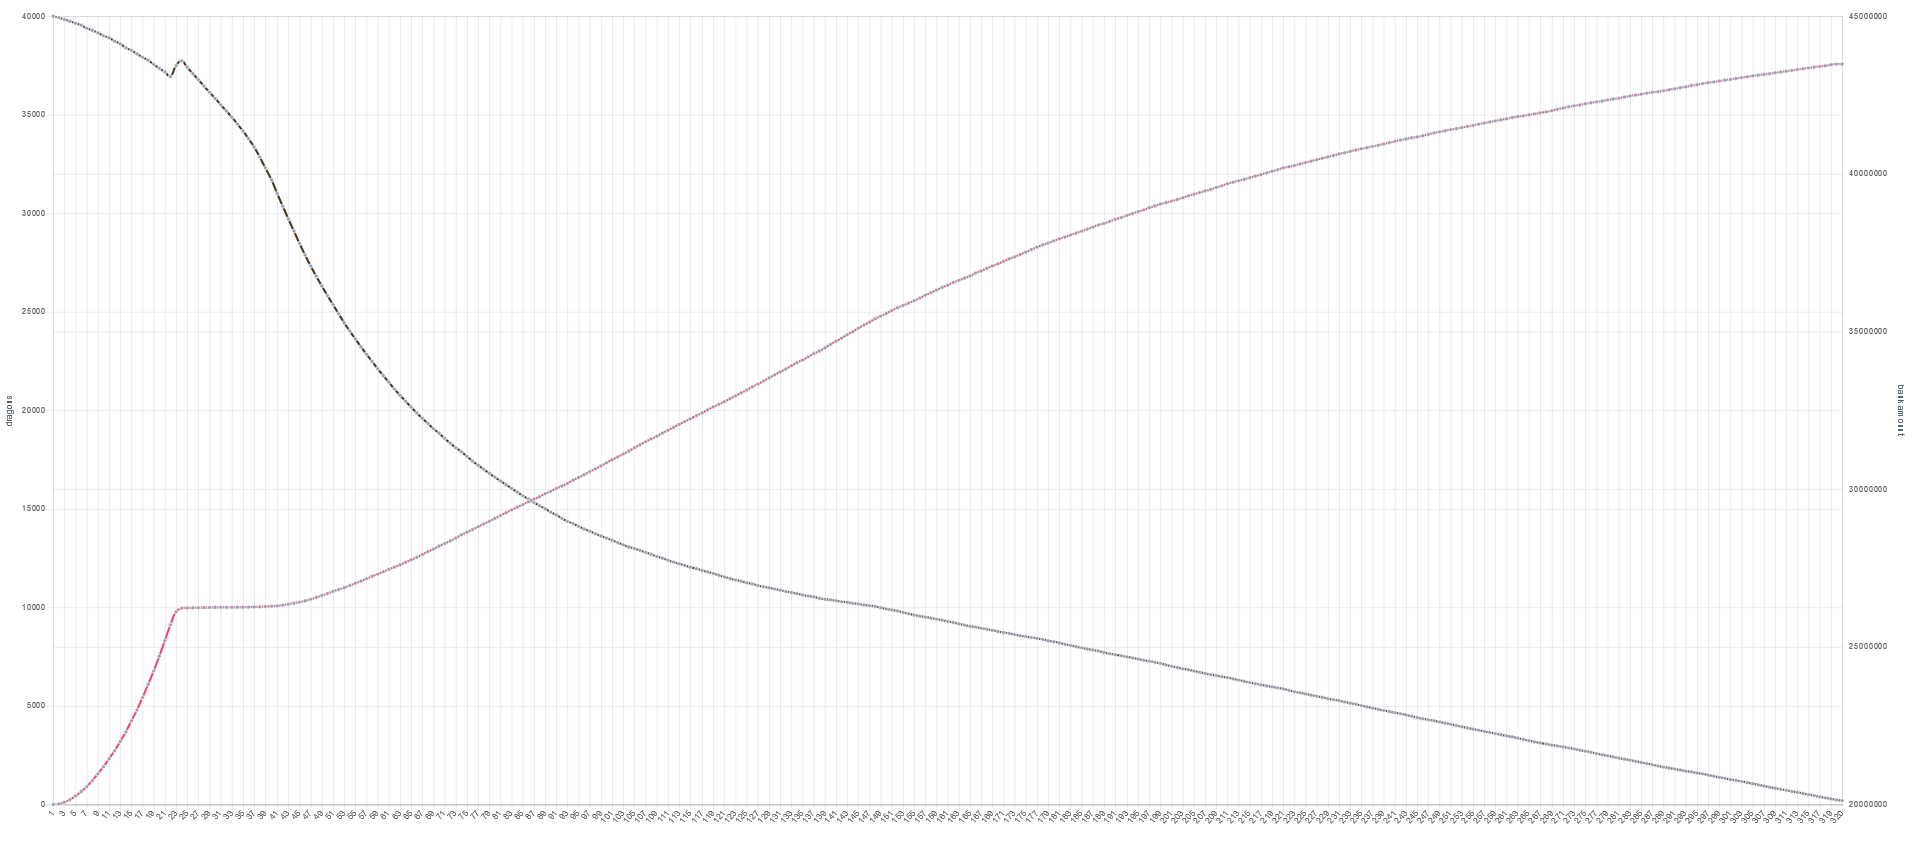
\includegraphics[width=6.27in,height=2.79in]{./media/CS1image1.png}
		\caption{The number of dragons (red line), and the Treasury balance in GOLD (black line)  as a function of the number of battles held.}
		\label{fig:The number of dragons (red line) as a function of the number of battles held, and the Treasury balance in GOLD (black line)}
	\end{Center}
\end{figure}


%%%%%%%%%%%%%%%%%%%% Figure/Image No: 9 Ends here %%%%%%%%%%%%%%%%%%%%


The \textit{battle winner reward} settles at 4.94 GOLD to 7.6 GOLD per battle depending on the DS\textit{.} This small range of reward values can be explained by the fact that all dragons are of similar DS since the players do not level up dragons and spend all DP on breeding. The exact values of the median \textit{battle winner reward }can be seen in  Table \ref{tab:Table showing the number of battles held (column 1), the corresponding dragon population (column 2), the Gold in the Treasury (column 3), the median battle winner reward (column 4), the median cost of Gold in $ (column 5), and the cost of an egg incubation (column 6).  This information is provided for the three different cases studied below. } (column 4), and Figure \ref{fig:The cost of Gold in dollars calculated as a sum of mining fees cost (light blue line), and the median battle reward in Gold versus the number of battles held (dark blue line).} (dark blue line).\par



%%%%%%%%%%%%%%%%%%%% Figure/Image No: 10 starts here %%%%%%%%%%%%%%%%%%%%

\begin{figure}[H]
	\begin{Center}
		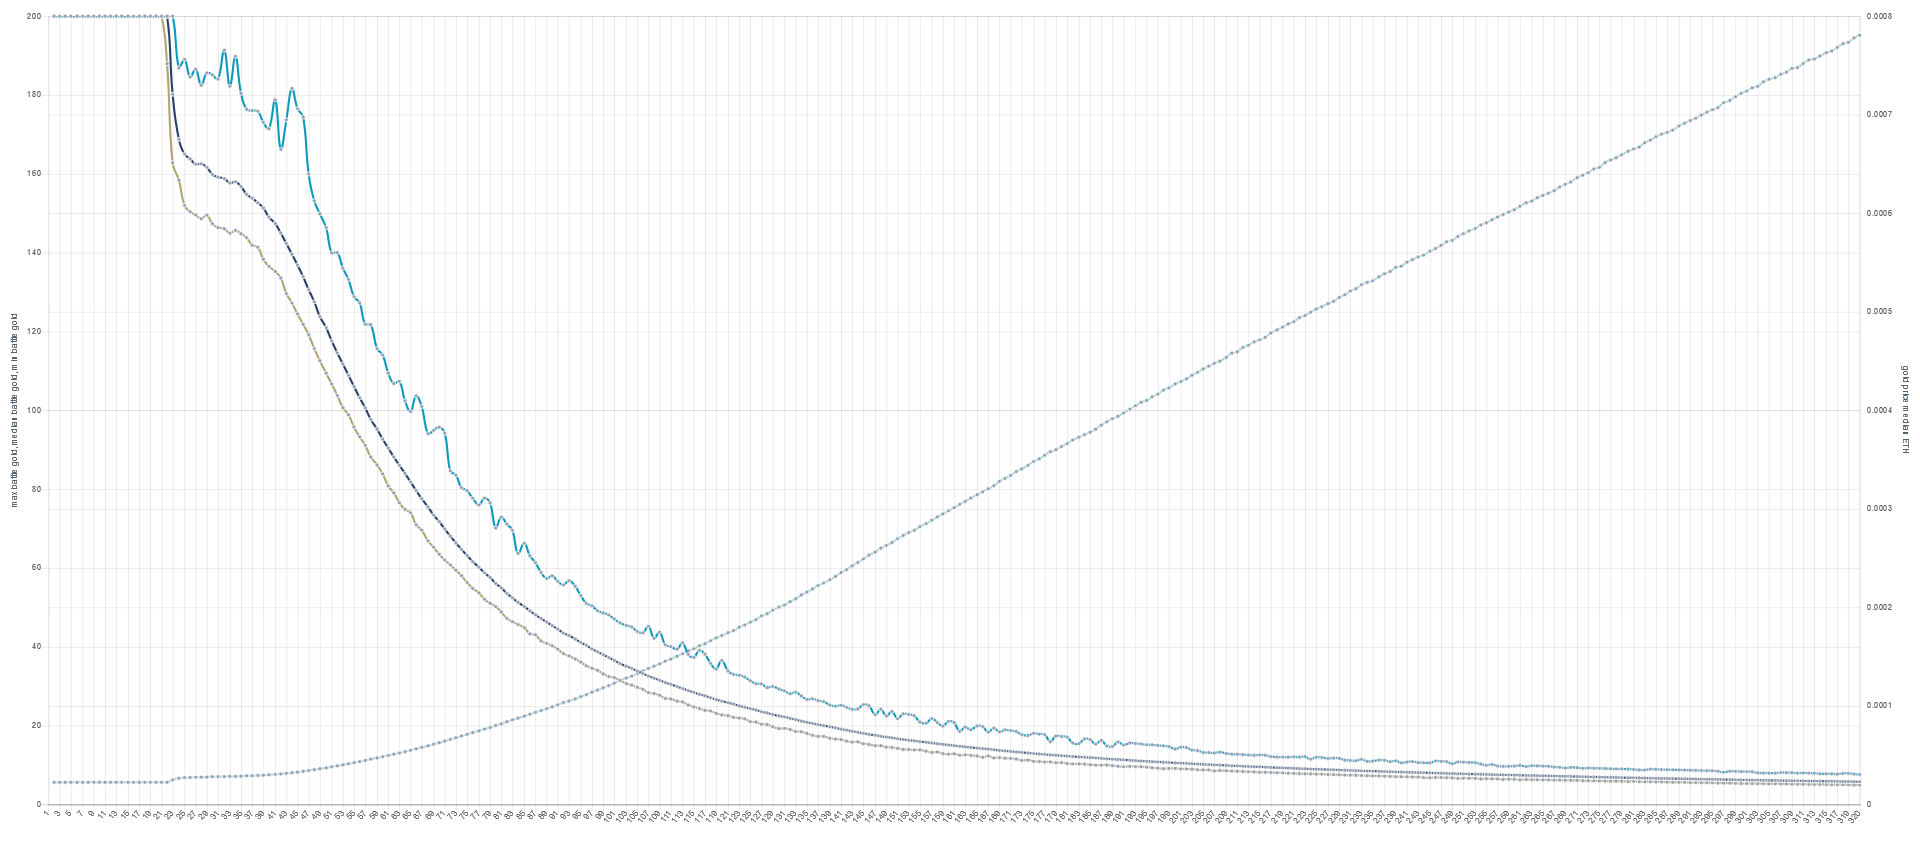
\includegraphics[width=6.27in,height=2.76in]{./media/CS1image2.png}
		\caption{The cost of Gold in ETH calculated as a sum of mining fees (light blue line), and the median {\it battle winner reward} in Gold versus the number of battles held (dark blue line). The minimum (brown line) and the maximum (cyan) {\it battle winner reward} are also shown encasing the median {\it battle winner reward}.}
		\label{fig:The cost of Gold in dollars calculated as a sum of mining fees cost (light blue line), and the median battle reward in Gold versus the number of battles held (dark blue line).}
	\end{Center}
\end{figure}


%%%%%%%%%%%%%%%%%%%% Figure/Image No: 10 Ends here %%%%%%%%%%%%%%%%%%%%


In Figure \ref{fig:The cost of Gold in dollars calculated as a sum of mining fees cost (light blue line), and the median battle reward in Gold versus the number of battles held (dark blue line).} the cost of Gold in ETH calculated as a sum of mining fees necessary to mine the corresponding transactions is shown (light blue line) versus the number of battles held, which just like in Figure \ref{fig:The number of dragons (red line) as a function of the number of battles held, and the Treasury balance in GOLD (black line)} is a variable that represents time in this synthetic environment. The cost of Gold grows because the amount of Gold distributed to winners reduces with the increasing number of battles held\ (see\ Section   \ref{Early adopter advantage}),\ making Gold more valuable.The median {\it battle winner reward} shown in the dark blue line decreases, as it depends on the amount of Gold in the Treasury, see Equation  \ref{Eq:R}, which also decreases as shown in Figure \ref{fig:The number of dragons (red line) as a function of the number of battles held, and the Treasury balance in GOLD (black line)}.\par

The mining cost for 1 GOLD is between 0.000591 ETH and 0.000909 ETH, at 3,000,000 battles, Figure \ref{fig:The cost of Gold in dollars calculated as a sum of mining fees cost (light blue line), and the median battle reward in Gold versus the number of battles held (dark blue line).} (light blue line).  It is calculated as:  ${{C}\over{\bar R}}$, where C is the cost of the transaction and  $\bar R$ is the median \textit{battle winner reward} (the median battle reward is shown as a function of the number of battles held in Figure \ref{fig:The cost of Gold in dollars calculated as a sum of mining fees cost (light blue line), and the median battle reward in Gold versus the number of battles held (dark blue line).}).\par

The cost of an egg incubation in this case is between 0.59 ETH and 0.91 ETH. This range comes from the fact that depending on who the winning dragons are there will be a different \textit{battle winner reward} associated with them depending on their DS.\par

Therefore, economically motivated players will start leveling up dragons in order to get dragons of higher DS and earn more Gold in battles. As such, Case 1 is not in a stable state and will eventually turn into Case 2 portrayed below.\par


\subsection{Case 2: Breeding and Leveling Up}
%\addcontentsline{toc}{subsection}{Case 2: Breeding and Leveling Up}
\label{Case 2: Breeding and Leveling Up} \par


%%%%%%%%%%%%%%%%%%%% Table No: 13 starts here %%%%%%%%%%%%%%%%%%%%


\begin{table}[H]
 			\centering
\begin{tabular}{p{0.6in}p{0.64in}p{0.55in}p{0.55in}p{0.99in}p{0.9in}p{0.99in}}
%row no:1
\hhline{-------}
%row no:2
\multicolumn{1}{|p{0.6in}}{{\fontsize{10pt}{12.0pt}\selectfont Number of Battles}} & 
\multicolumn{1}{|p{0.64in}}{{\fontsize{10pt}{12.0pt}\selectfont Population}} & 
\multicolumn{1}{|p{0.55in}}{{\fontsize{10pt}{12.0pt}\selectfont Treasury (GOLD)}} & 
\multicolumn{1}{|p{0.55in}}{{\fontsize{10pt}{12.0pt}\selectfont Supply (GOLD)}} & 
\multicolumn{1}{|p{0.99in}}{{\fontsize{10pt}{12.0pt}\selectfont Median battle reward (GOLD)}} & 
\multicolumn{1}{|p{0.9in}}{{\fontsize{10pt}{12.0pt}\selectfont Median cost of Gold (ETH)}} & 
\multicolumn{1}{|p{0.99in}|}{{\fontsize{10pt}{12.0pt}\selectfont Cost of egg incubation (ETH)}} \\
\hhline{-------}
%row no:3
\multicolumn{1}{|p{0.6in}}{\raggedleft {\fontsize{10pt}{12.0pt}\selectfont 500000}} & 
\multicolumn{1}{|p{0.64in}}{\raggedleft {\fontsize{10pt}{12.0pt}\selectfont 12500}} & 
\multicolumn{1}{|p{0.55in}}{\raggedleft {\fontsize{10pt}{12.0pt}\selectfont 18010000}} & 
\multicolumn{1}{|p{0.55in}}{\raggedleft {\fontsize{10pt}{12.0pt}\selectfont 43750000}} & 
\multicolumn{1}{|p{0.99in}}{\raggedleft {\fontsize{10pt}{12.0pt}\selectfont 51.18}} & 
\multicolumn{1}{|p{0.9in}}{\raggedleft {\fontsize{10pt}{12.0pt}\selectfont 0.000088}} & 
\multicolumn{1}{|p{0.99in}|}{\raggedleft {\fontsize{10pt}{12.0pt}\selectfont 0.088}} \\
\hhline{-------}
%row no:4
\multicolumn{1}{|p{0.6in}}{\raggedleft {\fontsize{10pt}{12.0pt}\selectfont 1000000}} & 
\multicolumn{1}{|p{0.64in}}{\raggedleft {\fontsize{10pt}{12.0pt}\selectfont 16000}} & 
\multicolumn{1}{|p{0.55in}}{\raggedleft {\fontsize{10pt}{12.0pt}\selectfont 10110000}} & 
\multicolumn{1}{|p{0.55in}}{\raggedleft {\fontsize{10pt}{12.0pt}\selectfont 42000000}} & 
\multicolumn{1}{|p{0.99in}}{\raggedleft {\fontsize{10pt}{12.0pt}\selectfont 20.50}} & 
\multicolumn{1}{|p{0.9in}}{\raggedleft {\fontsize{10pt}{12.0pt}\selectfont 0.000219}} & 
\multicolumn{1}{|p{0.99in}|}{\raggedleft {\fontsize{10pt}{12.0pt}\selectfont 0.219}} \\
\hhline{-------}
%row no:5
\multicolumn{1}{|p{0.6in}}{\raggedleft {\fontsize{10pt}{12.0pt}\selectfont 1500000}} & 
\multicolumn{1}{|p{0.64in}}{\raggedleft {\fontsize{10pt}{12.0pt}\selectfont 19600}} & 
\multicolumn{1}{|p{0.55in}}{\raggedleft {\fontsize{10pt}{12.0pt}\selectfont 6980000}} & 
\multicolumn{1}{|p{0.55in}}{\raggedleft {\fontsize{10pt}{12.0pt}\selectfont 40200000}} & 
\multicolumn{1}{|p{0.99in}}{\raggedleft {\fontsize{10pt}{12.0pt}\selectfont 10.72}} & 
\multicolumn{1}{|p{0.9in}}{\raggedleft {\fontsize{10pt}{12.0pt}\selectfont 0.000419}} & 
\multicolumn{1}{|p{0.99in}|}{\raggedleft {\fontsize{10pt}{12.0pt}\selectfont 0.419}} \\
\hhline{-------}
%row no:6
\multicolumn{1}{|p{0.6in}}{\raggedleft {\fontsize{10pt}{12.0pt}\selectfont 2000000}} & 
\multicolumn{1}{|p{0.64in}}{\raggedleft {\fontsize{10pt}{12.0pt}\selectfont 22900}} & 
\multicolumn{1}{|p{0.55in}}{\raggedleft {\fontsize{10pt}{12.0pt}\selectfont 5550000}} & 
\multicolumn{1}{|p{0.55in}}{\raggedleft {\fontsize{10pt}{12.0pt}\selectfont 38500000}} & 
\multicolumn{1}{|p{0.99in}}{\raggedleft {\fontsize{10pt}{12.0pt}\selectfont 6.70}} & 
\multicolumn{1}{|p{0.9in}}{\raggedleft {\fontsize{10pt}{12.0pt}\selectfont 0.000672}} & 
\multicolumn{1}{|p{0.99in}|}{\raggedleft {\fontsize{10pt}{12.0pt}\selectfont 0.672}} \\
\hhline{-------}
%row no:7
\multicolumn{1}{|p{0.6in}}{\raggedleft {\fontsize{10pt}{12.0pt}\selectfont 2500000}} & 
\multicolumn{1}{|p{0.64in}}{\raggedleft {\fontsize{10pt}{12.0pt}\selectfont 26400}} & 
\multicolumn{1}{|p{0.55in}}{\raggedleft {\fontsize{10pt}{12.0pt}\selectfont 4970000}} & 
\multicolumn{1}{|p{0.55in}}{\raggedleft {\fontsize{10pt}{12.0pt}\selectfont 36800000}} & 
\multicolumn{1}{|p{0.99in}}{\raggedleft {\fontsize{10pt}{12.0pt}\selectfont 4.75}} & 
\multicolumn{1}{|p{0.9in}}{\raggedleft {\fontsize{10pt}{12.0pt}\selectfont 0.000948}} & 
\multicolumn{1}{|p{0.99in}|}{\raggedleft {\fontsize{10pt}{12.0pt}\selectfont 0.948}} \\
\hhline{-------}
%row no:8
\multicolumn{1}{|p{0.6in}}{\raggedleft {\fontsize{10pt}{12.0pt}\selectfont 3000000}} & 
\multicolumn{1}{|p{0.64in}}{\raggedleft {\fontsize{10pt}{12.0pt}\selectfont 29300}} & 
\multicolumn{1}{|p{0.55in}}{\raggedleft {\fontsize{10pt}{12.0pt}\selectfont 4620000}} & 
\multicolumn{1}{|p{0.55in}}{\raggedleft {\fontsize{10pt}{12.0pt}\selectfont 35330000}} & 
\multicolumn{1}{|p{0.99in}}{\raggedleft {\fontsize{10pt}{12.0pt}\selectfont 3.69}} & 
\multicolumn{1}{|p{0.9in}}{\raggedleft {\fontsize{10pt}{12.0pt}\selectfont 0.001217}} & 
\multicolumn{1}{|p{0.99in}|}{\raggedleft {\fontsize{10pt}{12.0pt}\selectfont 1.217}} \\
\hhline{-------}

\end{tabular}\caption{Case Study 2: the number of battles held (column 1), the corresponding dragon population (column 2), the Gold in the Treasury (column 3), Gold supply (column 4), the median {\it battle winner reward} (column 5), the median cost of Gold in ETH (column 6), and the cost of an egg incubation in ETH (column 7).}
\label{tab:Same as Table 11, but for Case Study 2}

 \end{table}


%%%%%%%%%%%%%%%%%%%% Table No: 13 ends here %%%%%%%%%%%%%%%%%%%%


In this scenario players randomly breed and level up dragons. In our opinion this is the most likely scenario.\par

The game balance drops to around 10M GOLD at 1,000,000 battles, however further decline is very slow and the ballance decreases to 4.6M GOLD at 3,000,000 battles and to 3.1M GOLD at 5,000,000 battles. The \textit{battle winner reward} settles between 1.99 GOLD and 10.21 GOLD per battle depending on the DS of the winning dragon at 3,000,000 battles.\par

In Figure \ref{fig:CS2The number of dragons (red line) as a function of the number of battles held, and the Treasury balance in Gold (black line).}, just as in Figure \ref{fig:The number of dragons (red line) as a function of the number of battles held, and the Treasury balance in GOLD (black line)} the initial sharp growth of the dragon population is due to the distribution of genesis eggs (red line). The black line shows the amount of Gold in the Treasury, which is declining due to the distribution of Gold to the battle winners and partial annihilation of Gold by the Nest.\par



%%%%%%%%%%%%%%%%%%%% Figure/Image No: 11 starts here %%%%%%%%%%%%%%%%%%%%

\begin{figure}[H]
	\begin{Center}
		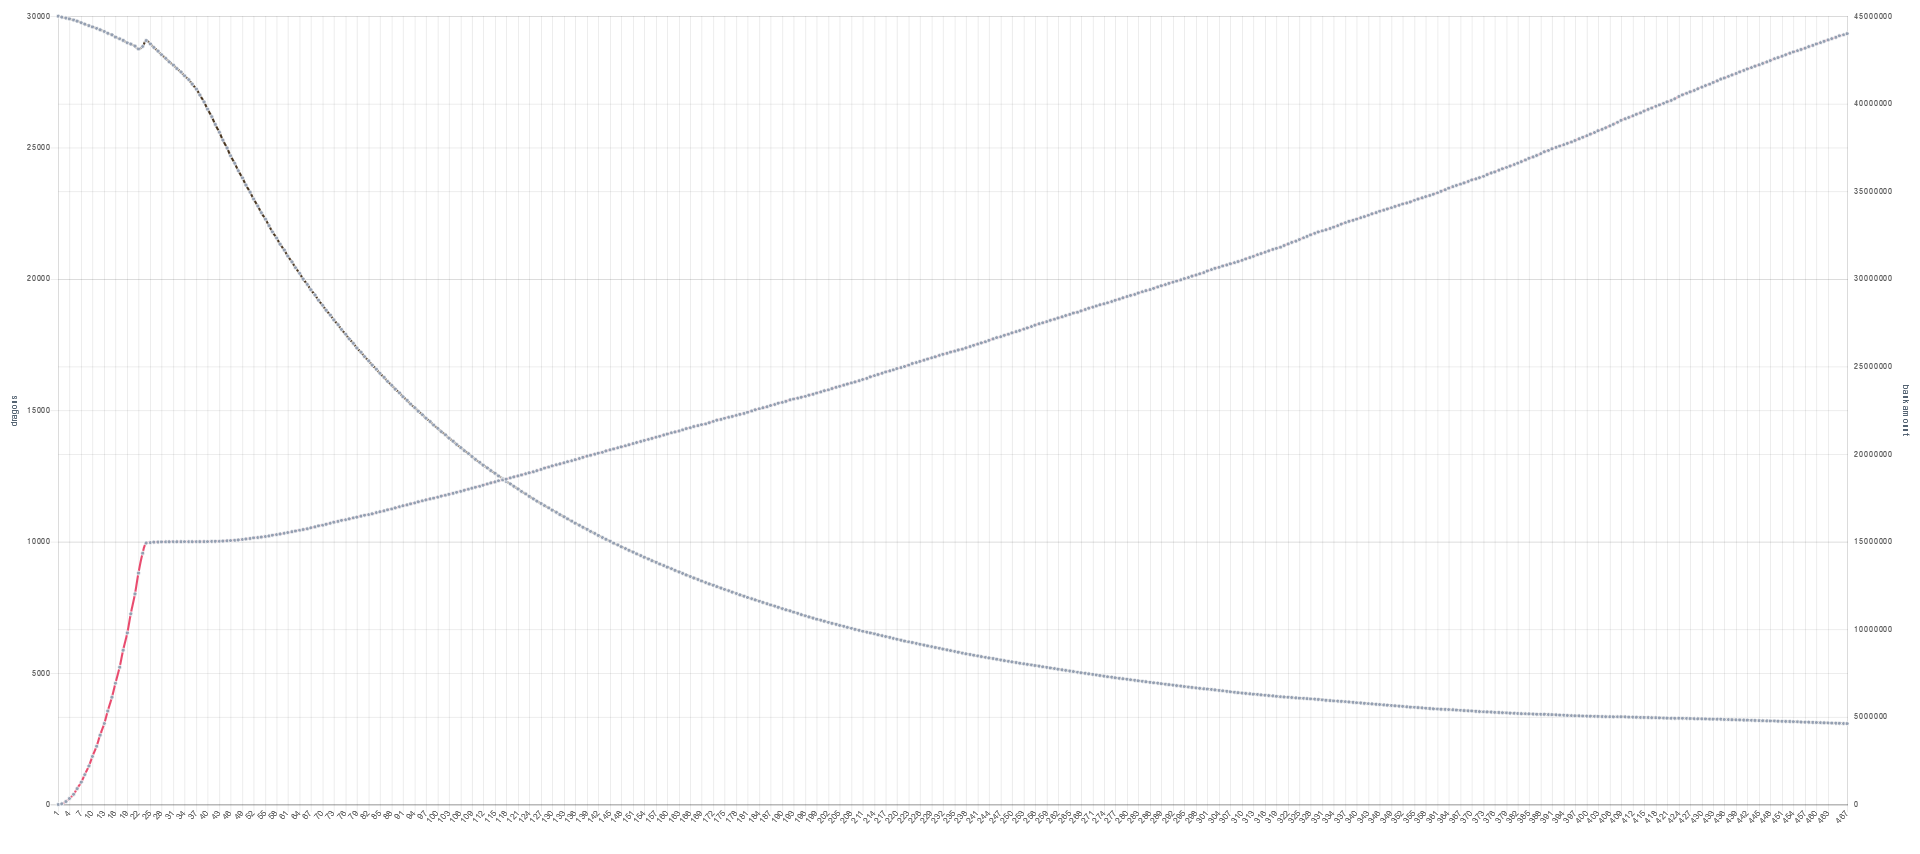
\includegraphics[width=6.27in,height=2.76in]{./media/CS2image1.png}
		\caption{The number of dragons (red line), and the Treasury balance in GOLD (black line) as a function of the number of battles held for Case Study 2.}
		\label{fig:CS2The number of dragons (red line) as a function of the number of battles held, and the Treasury balance in Gold (black line).}
	\end{Center}
\end{figure}


%%%%%%%%%%%%%%%%%%%% Figure/Image No: 11 Ends here %%%%%%%%%%%%%%%%%%%%



%%%%%%%%%%%%%%%%%%%% Figure/Image No: 12 starts here %%%%%%%%%%%%%%%%%%%%

\begin{figure}[H]
	\begin{Center}
		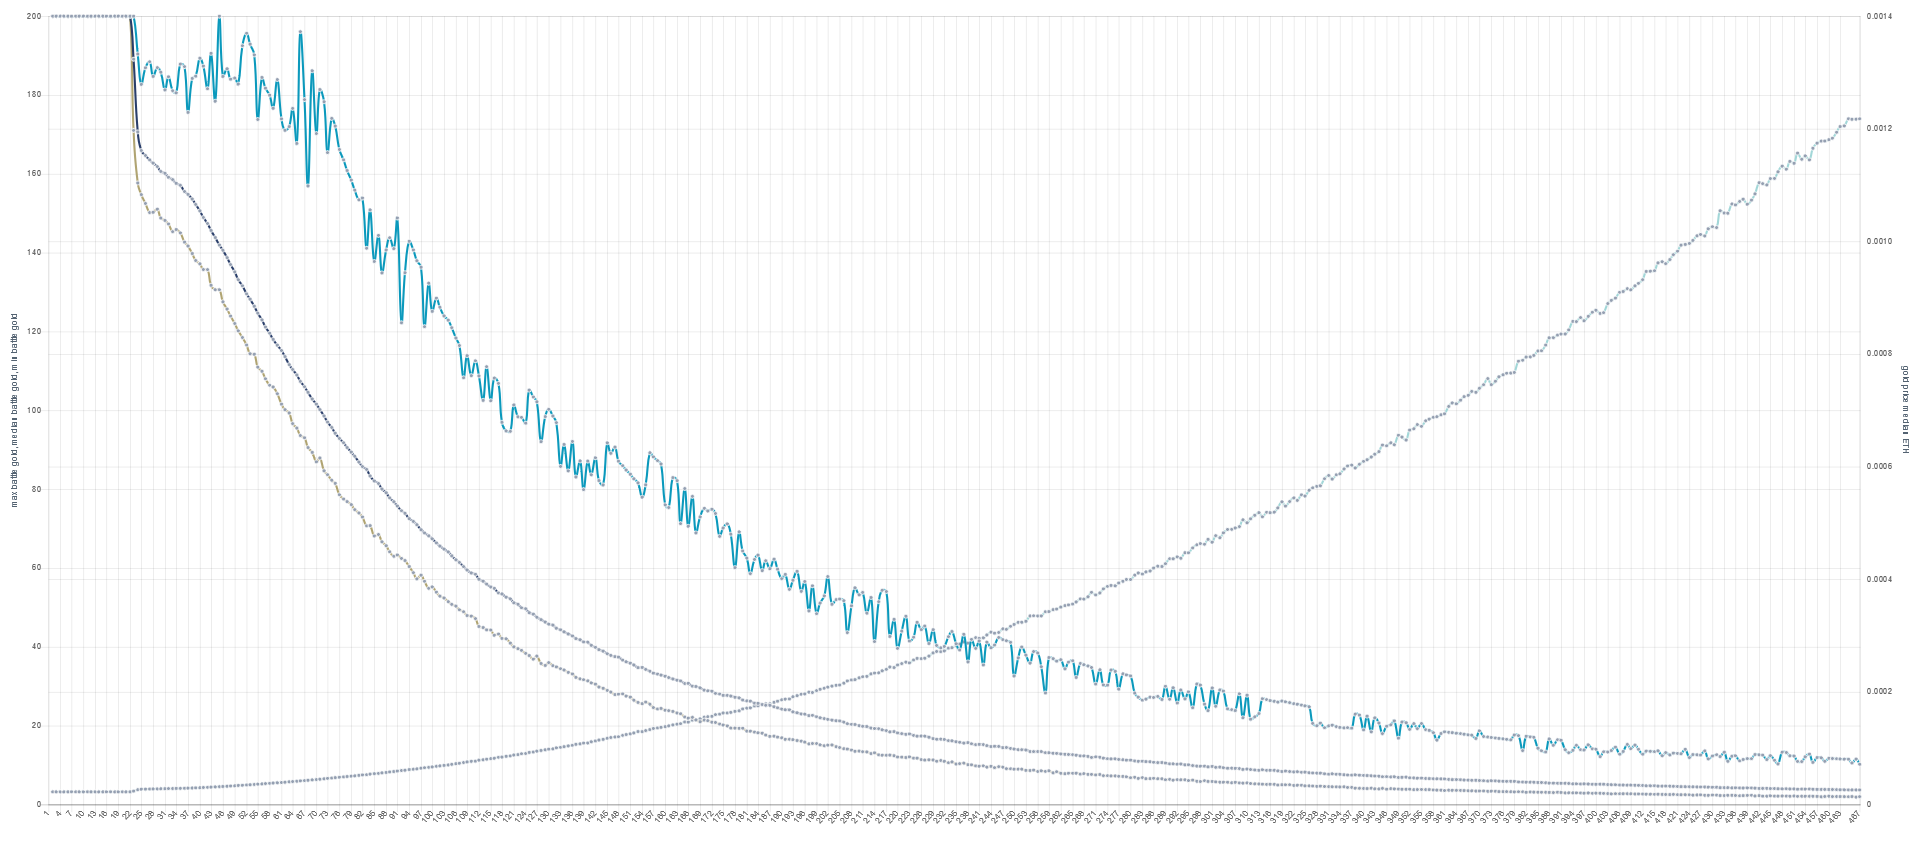
\includegraphics[width=6.27in,height=2.76in]{./media/CS2image2.png}
		\caption{The cost of Gold in ETH calculated as a sum of mining fees (light blue line), and the median {\it battle winner reward} in Gold versus the number of battles held (dark blue line) for Case Study 2. The minimum (brown line) and the maximum (cyan) {\it battle winner reward} are also shown encasing the median {\it battle winner reward}.}
		\label{The cost of Gold in dollars calculated as a mining fee (light blue line), and the median battle reward in Gold versus the number of battles held (dark blue line).}
	\end{Center}
\end{figure}


%%%%%%%%%%%%%%%%%%%% Figure/Image No: 12 Ends here %%%%%%%%%%%%%%%%%%%%


The mining cost for 1 GOLD is between 0.000441 ETH and 0.002257 ETH, at 3,000,000 battles, see Table \ref{tab:Same as Table 11, but for Case Study 2} (column 5), and Figure \ref{The cost of Gold in dollars calculated as a mining fee (light blue line), and the median battle reward in Gold versus the number of battles held (dark blue line).} (light blue line). The value of the mining cost will continue to grow with the increasing number of dragons and the \textit{battle winner reward} will be reduced as was described in Section \ref{Early adopter advantage}. The egg incubation cost in this case is between 0.44 ETH and 2.26 ETH. This variation is due to the fact that each dragon has a corresponding DS, on which the {\it battle winner reward} depends (see Equation \ref{Eq:R}), so the {\it battle winner reward} will depend on which dragons are fighting at a given time, and the possible price of the egg incubation will have a spread depending on all the different possibilities. It should also be noted that in Figure \ref{The cost of Gold in dollars calculated as a mining fee (light blue line), and the median battle reward in Gold versus the number of battles held (dark blue line).}, the maximum {\it battle winner reward} fluctuates due to the fact that it depends on the DS of the participating dragons. Therefore, if certain dragons with high DS are not participating in battles at some points this will affect the value of the maximum {\it battle winner reward}.\par


\subsection{Case 3: Predominantly Leveling Up}
%\addcontentsline{toc}{subsection}{Case 3: Predominantly Leveling Up}
\label{Case 3: Predominantly Leveling Up} \par


%%%%%%%%%%%%%%%%%%%% Table No: 14 starts here %%%%%%%%%%%%%%%%%%%%


\begin{table}[H]
 			\centering
\begin{tabular}{p{0.6in}p{0.64in}p{0.55in}p{0.55in}p{0.99in}p{0.9in}p{0.99in}}
%row no:1
\hhline{-------}
%row no:2
\multicolumn{1}{|p{0.6in}}{{\fontsize{10pt}{12.0pt}\selectfont Number of Battles}} & 
\multicolumn{1}{|p{0.64in}}{{\fontsize{10pt}{12.0pt}\selectfont Population}} & 
\multicolumn{1}{|p{0.55in}}{{\fontsize{10pt}{12.0pt}\selectfont Treasury (GOLD)}} & 
\multicolumn{1}{|p{0.55in}}{{\fontsize{10pt}{12.0pt}\selectfont Supply (GOLD)}} & 
\multicolumn{1}{|p{0.99in}}{{\fontsize{10pt}{12.0pt}\selectfont Median battle reward (GOLD)}} & 
\multicolumn{1}{|p{0.9in}}{{\fontsize{10pt}{12.0pt}\selectfont Median cost of Gold (ETH)}} & 
\multicolumn{1}{|p{0.99in}|}{{\fontsize{10pt}{12.0pt}\selectfont Cost of egg incubation (ETH)}} \\
\hhline{-------}
%row no:3
\multicolumn{1}{|p{0.6in}}{\raggedleft {\fontsize{10pt}{12.0pt}\selectfont 500000}} & 
\multicolumn{1}{|p{0.64in}}{\raggedleft {\fontsize{10pt}{12.0pt}\selectfont 10000}} & 
\multicolumn{1}{|p{0.55in}}{\raggedleft {\fontsize{10pt}{12.0pt}\selectfont 14010000}} & 
\multicolumn{1}{|p{0.55in}}{\raggedleft {\fontsize{10pt}{12.0pt}\selectfont 45000000}} & 
\multicolumn{1}{|p{0.99in}}{\raggedleft {\fontsize{10pt}{12.0pt}\selectfont 66.69}} & 
\multicolumn{1}{|p{0.9in}}{\raggedleft {\fontsize{10pt}{12.0pt}\selectfont 0.000067}} & 
\multicolumn{1}{|p{0.99in}|}{\raggedleft {\fontsize{10pt}{12.0pt}\selectfont 0.067}} \\
\hhline{-------}
%row no:4
\multicolumn{1}{|p{0.6in}}{\raggedleft {\fontsize{10pt}{12.0pt}\selectfont 1000000}} & 
\multicolumn{1}{|p{0.64in}}{\raggedleft {\fontsize{10pt}{12.0pt}\selectfont 10190}} & 
\multicolumn{1}{|p{0.55in}}{\raggedleft {\fontsize{10pt}{12.0pt}\selectfont 2497000}} & 
\multicolumn{1}{|p{0.55in}}{\raggedleft {\fontsize{10pt}{12.0pt}\selectfont 44900000}} & 
\multicolumn{1}{|p{0.99in}}{\raggedleft {\fontsize{10pt}{12.0pt}\selectfont 16.86}} & 
\multicolumn{1}{|p{0.9in}}{\raggedleft {\fontsize{10pt}{12.0pt}\selectfont 0.000267}} & 
\multicolumn{1}{|p{0.99in}|}{\raggedleft {\fontsize{10pt}{12.0pt}\selectfont 0.267}} \\
\hhline{-------}
%row no:7
\multicolumn{1}{|p{0.6in}}{\raggedleft {\fontsize{10pt}{12.0pt}\selectfont 1500000}} & 
\multicolumn{1}{|p{0.64in}}{\raggedleft {\fontsize{10pt}{12.0pt}\selectfont 11250}} & 
\multicolumn{1}{|p{0.55in}}{\raggedleft {\fontsize{10pt}{12.0pt}\selectfont 0}} & 
\multicolumn{1}{|p{0.55in}}{\raggedleft {\fontsize{10pt}{12.0pt}\selectfont 44370000}} & 
\multicolumn{1}{|p{0.99in}}{\raggedleft {\fontsize{10pt}{12.0pt}\selectfont 0}} & 
\multicolumn{1}{|p{0.9in}}{{\fontsize{10pt}{12.0pt}\selectfont Determined by the market}} & 
\multicolumn{1}{|p{0.99in}|}{{\fontsize{10pt}{12.0pt}\selectfont Determined by the market}} \\
\hhline{-------}

\end{tabular}\caption{Case Study 3: the number of battles held (column 1), the corresponding dragon population (column 2), the Gold in the Treasury (column 3), Gold supply (column 4), the median {\it battle winner reward} (column 5), the median cost of Gold in ETH (column 6), and the cost of an egg incubation in ETH (column 7).}
\label{tab:Same as Table 11, but for Case Study 3}

 \end{table}


%%%%%%%%%%%%%%%%%%%% Table No: 14 ends here %%%%%%%%%%%%%%%%%%%%


In this scenario players level up dragons on all levels with a 90$\%$  probability and breed with a 10$\%$  probability.\par

The game balance drops to 0 GOLD at approximately 1,430,000 battles, as a result of the low amount of fees collected for egg incubations, as is seen in Figure \ref{fig:The number of dragons (red line), and the Treasury balance in Gold (black line) as a function of the number of battles held for Case Study 3.}}, and in column 3 of  Table \ref{tab:Same as Table 11, but for Case Study 3}. Therefore the \textit{battle winner reward} will not be paid. This is shown in Figure \ref{fig:The median battle reward in Gold versus the number of battles held (dark blue line) for Case Study 3.}, where the {\it battle winner reward} drops sharply to zero with the number of battles held (dark blue line). Just before that moment the median {\it battle winner reward} will be 0.13 GOLD, and the median mining cost of Gold will be 0.022573 ETH.  Once the game balance is at 0 GOLD, the price of Gold cannot be predicted due to the fact that when there is no Gold in the Treasury, the model assumes that the price of Gold is equal to the transaction fees price divided by zero (or another very small amount), thus making it too big to display on the graph. \par



%%%%%%%%%%%%%%%%%%%% Figure/Image No: 13 starts here %%%%%%%%%%%%%%%%%%%%

\begin{figure}[H]
	\begin{Center}
		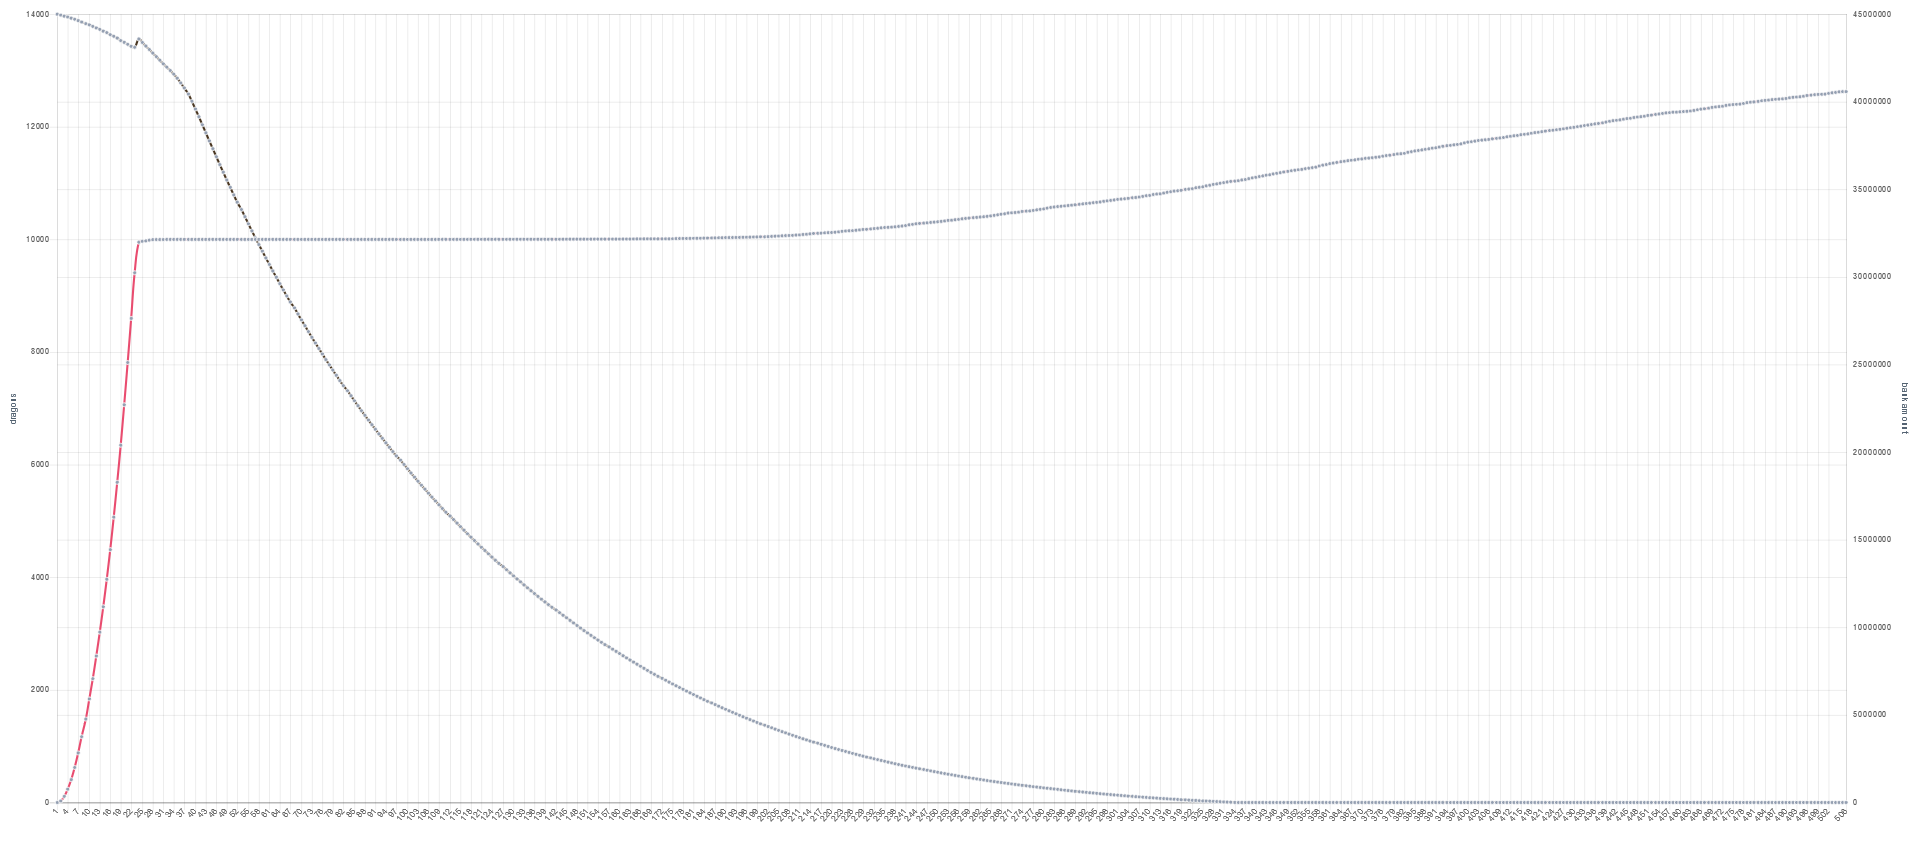
\includegraphics[width=6.27in,height=2.78in]{./media/CS3image1.png}
		\caption{The number of dragons (red line), and the Treasury balance in GOLD (black line) as a function of the number of battles held for Case Study 3.}
		\label{fig:The number of dragons (red line), and the Treasury balance in Gold (black line) as a function of the number of battles held for Case Study 3.}
	\end{Center}
\end{figure}


%%%%%%%%%%%%%%%%%%%% Figure/Image No: 13 Ends here %%%%%%%%%%%%%%%%%%%%


Gold can be obtained from other players and therefore its price can not be determined by this simulation. The egg incubation cost also goes up and becomes unfeasible for the majority of players.\par



%%%%%%%%%%%%%%%%%%%% Figure/Image No: 14 starts here %%%%%%%%%%%%%%%%%%%%

\begin{figure}[H]
	\begin{Center}
		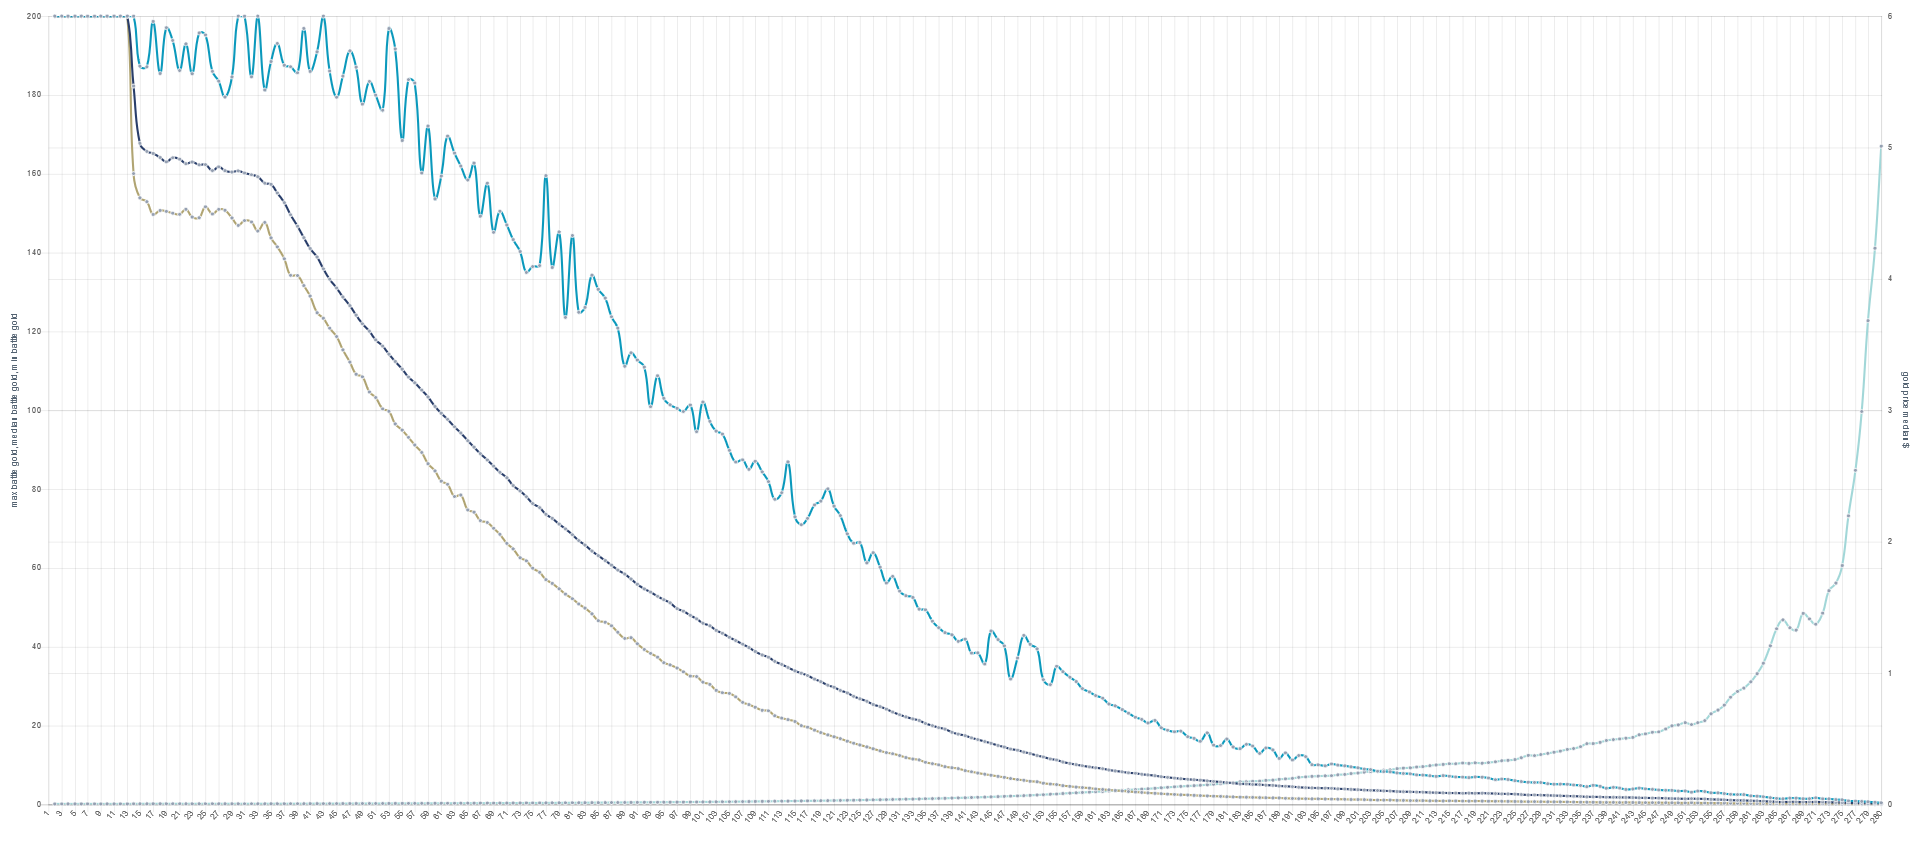
\includegraphics[width=6.27in,height=2.78in]{./media/CS3image2.png}
        \caption{The cost of Gold in ETH calculated as a sum of mining fees (light blue line), and the median {\it battle winner reward} in Gold versus the number of battles held (dark blue line) for Case Study 3. The minimum (brown line) and the maximum (cyan) {\it battle winner reward} are also shown encasing the median {\it battle winner reward}.}
		\label{fig:The median battle reward in Gold versus the number of battles held (dark blue line) for Case Study 3.}
	\end{Center}
\end{figure}


%%%%%%%%%%%%%%%%%%%% Figure/Image No: 14 Ends here %%%%%%%%%%%%%%%%%%%%


Therefore, the game slows down and new dragons can only be hatched with the Gold bought on the marketplace. However, this is not critical as the initial \textit{battle winner reward }is not a goal of the game but just a mechanism to start up the in-game economy. Our aim is the creation of the game ecosystem where users will offer different goods and services to each other and those goods and services will be exchanged for Gold (healing, buffs) or acquired with the help of Gold (bets on dragon battles).\par

Additionally, as the price of dragons will become higher more players will switch to breeding dragons therefore bringing the game to the state portrayed in Case 2.\par

These synthetic tests confirm that the aim to create a game ecosystem which is stable in the long term was achieved. The explored scenarios might not include all the possible options for the players’ behaviour, nonetheless, they offer an insight on how the game ecosystem might develop after the launch. It is shown that due to the system of feedback loops implemented in the game, that all three cases are going to end up in the equilibrium state of Case Study 2.\par

 %%%%%%%%%%%%  Starting New Page here %%%%%%%%%%%%%%

\newpage

\vspace{\baselineskip}\section{Implementation Details}
%\addcontentsline{toc}{section}{Implementation Details}
\label{Implementation Details}  \par

\subsection{Serverless application}
%\addcontentsline{toc}{subsection}{Serverless application}
\label{Serverless application} \par

Modern centralized games heavily rely on the entities that have created those games and that have full control over every aspect of the game: what to consider as a $``$bad$"$  or $``$good$"$  behaviour, private data policies, controls over the servers and all the data stored there, and determining the overall direction of the game development  \cite{Gogo_2018_Jun_16},  \cite{Steam_2017},  \cite{WikipediA_2018}\footnote{Sort the table by organization type (3rd column) and see the gaming entries.}, \cite{Ben_Gilbert_2018_Jun_22},  \cite{Aaron_Mamiit__2017_Mar_30}.\par

At the same time a number of technologies unrelated to the gaming industry has been emerging which let users enjoy a transparent, censorship resistant, trustless, programmable and permissionless environment where anyone has full control over their private data (this technology stack is often referred to as Web 3.0  \cite{Josh_Stark_2018_Jun_6},  \cite{Stephan_Tual_2017_May_26}.)\par

We think that it would be great to create a full scale game built on top of those technologies, so the created game will be 100$\%$  autonomous and decentralized, and no party will have control over any element of the game or its delivery mechanisms once it is launched, while still remaining engaging and fun compared to its centralized siblings.\par

However, with Dragonereum our aim is more realistic and it is to create a decentralized game which will have minimal ties to our servers at launch and gradually move to decentralized solutions (storage, naming services and indexing) once the game is released.\par

At game's launch we will retain the possibility to update and pause smart contracts in case of a critical bug or game balance issues. However, once the smart contracts will be battle-tested and all necessary security measures will be taken, the control over deployed smart contracts will be voluntarily transferred to a new owner. This might be a DAO or just the 0x000..0001 address.\par

\begin{samepage}
The upgrade mechanism works as follows:\par

\begin{itemize}
\item A new version of a required smart contract is deployed.\par

\item Ownership of this contract is transfered to UpgradeController.\par

\item Migrate function with old and new smart contracts is called by our multisig address.
\end{itemize}\par
\end{samepage}

In the long run and with the advancement of technology, we hope to remove any user dependency on us or on any other third party and switch to a fully autonomous and decentralized mode.\par

The game is currently accessible via browser with a MetaMask plugin installed (\href{https://metamask.io/}{\textcolor[HTML]{1155CC}{\uline{https://metamask.io/}}}), in Opera beta mobile browser, Status (\href{https://status.im/}{\textcolor[HTML]{1155CC}{\uline{https://status.im/}}}) and Cyb.\par

No sign up or any kind of registration is\ required as in order to offer engaging gameplay no one  needs to know the names or any other personal information of the players. The private keys which are stored in user's wallet are sufficient to serve as the players’ IDs.\par

The data layer consists of two ERC721  \cite{Ethereum_2017_Sep_26}  non-fungible tokens which will represent two states of a dragon (an egg and a dragon) and an ERC20  \cite{Ethereum_2015_Nov_19}  which will represent the in-game cryptocurrency. \par

The business logic layer consists of several smart contracts: egg core features contract, dragon core features contract, breeding, battling and marketplace contract.\par

The game itself can be used without reliance on a back-end server for any purposes other than allowing users to derive the app from the server to the player’s browser. The app uses client-side rendering, therefore, our server is actually just a storage which can be easily replaced.\par

\begin{samepage}
However, to make the life of players a bit easier another back-end server is used for:\par

\begin{itemize}
	\item Filtering of items offered on marketplaces.\par

	\item Opponent matchmaking for regular battles.\par

	\item Storage and delivery of notifications while a player is not online.
\end{itemize}\par
\end{samepage}

While the filtering server stores complete information about every item offered on the game’s marketplaces, the client side application only receives the list of items in a required order. This feature can easily be turned off in the app settings so the app can be used without it.\par

Full scale decentralization is our long term goal and once the game has all the core functionality we hope that new solutions and services from a Web 3.0 stack will be implemented.

 %%%%%%%%%%%%  Starting New Page here %%%%%%%%%%%%%%

%\newpage

\vspace{\baselineskip}\subsection{Off-chain solutions}
%\addcontentsline{toc}{subsection}{Off-chain solutions}
 \label{Off-chain solutions} \par

In Section \ref{Game Design Constraints} we discussed the current limitations associated with decentralized technologies and explained the steps taken in building Dragonereum with these limitations in mind. Another possible way of resolving the effects of the transaction costs, the associated delays with transaction processing and network congestion issues on the Ethereum network is with the use of off-chain (state-chain) solutions. We studied in detail the following most promising off-chain approaches for resolving the scalability issue:\par

\begin{itemize}
	\item State channels \cite{Joseph_Poon_et_al_2016}\par

	\item Sharding \cite{Vitalik_Buterin_2016}\par

	\item Plasma \cite{Josh_Stark__2018_February_12}\par

	\item TrueBit \cite{Jason_Teutsch_et_al_2017}, \cite{Julia_Koch_et_al_2018}\par

	\item zk-SNARKS off-chain validation(ZoKrates) \cite{Jacob_Eberhardt_2018}\par

	\item Sidechains \cite{Adam_Back_et_al_2014}\par
	
	\item POA network \cite{Stephen_Arsenault_2018}
\end{itemize}\par


\vspace{\baselineskip}
After\ carefully investigating the above off-chain solutions, we have concluded that at present they do not offer a viable solution for our game design, as many of them are not production ready yet and those in production do not have wide user base. As our game design was built with the current limitations of Ethereum’s blockchain bandwidth in mind, at this stage there is no real necessity to go off-chain. \par

Furthermore, by staying on-chain we have the advantage of remaining more secure, while the above third-party solutions might have certain vulnerabilities associated with them, especially if they have not been released and tested out yet. Another benefit from not relying on third parties is the fact that our system will not become dependent on solutions that might be suspended or abandoned at any point in time and, as a result, dragons will be immortal and will live forever. \par


 %%%%%%%%%%%%  Starting New Page here %%%%%%%%%%%%%%

%\newpage

\vspace{\baselineskip}\subsection{Graphics}
%\addcontentsline{toc}{subsection}{Graphics}
  \label{Graphics}  \par

While designing the game we considered several options for visualisation style of our dragons. Current status quo in cryptocollectible industry is  use of flat, simplified images which are easily merged into an image of a game character.\par

However, we decided to switch to 3/4 view as it gives more realistic perspective to players and it makes the potential transition to VR or AR a bit easier.

 %%%%%%%%%%%%  Starting New Page here %%%%%%%%%%%%%%

\newpage
\par

\section{Possible Integrations}
%\addcontentsline{toc}{section}{Possible Integrations}
 \label{Possible Integrations}  \par


\vspace{\baselineskip}
\subsection{Trading protocols}\label{Trading protocols}\par

In addition to the in-house marketplaces for game tokens such as dragon eggs (ERC721), dragons (ERC721) and Gold (ERC20) the decentralized nature of the tokens will allow them to be traded on other global trading platforms.\par

We prefer this to happen in an open and decentralized manner as all the information about each token is publicly accessible and there is no need to rely on any third party. Therefore, the best option for this is the decentralized liquidity networks and exchanges.\par

Joining the decentralized liquidity network Bancor will provide instant liquidity for Gold and enable its convertibility to other connected tokens and vice versa with low fees and no trading spread.\par

Additionally, all game tokens are compliant with the 0x’s protocol V2 therefore all of them can be traded on 0x relayers when V2 of 0x’s protocol will be launched.\par

The compliance of Dragonereum’s ERC721 tokens with the Wyvern Protocol (\url{https://www.projectwyvern.com/}) will enable gas-free and escrow-free auctions (sell orders) on platforms such as Opensea.io.\par

At game's launch there will be basic solution for in-game ERC20 trading, however we will consider implementing advanced solutions at a later date.\par


\vspace{\baselineskip}
\subsection{Prediction markets}\label{Prediction markets}\par

There are many game events which can be used as a base for a prediction, for example, battle winners and leaderboard entrants. Since in Dragonereum everything is kept on-chain, third-party services such as Augur (\url{https://www.augur.net/}) can be used to place bets on events and outcomes stored in the game’s smart contracts (even those that we can not predict at the moment).\par

With the current implementation of the Augur ecosystem we do not see the possibility to bet on small events (such as the outcome of a regular battle), however, other betting services (DiceyBit \url{https://diceybit.com}) already offer those capabilities with the use of data supplied by the game developers through an API. On the other hand, Augur can be used for larger scale events, such as predicting the maximum Dragon Skillfulness Index at a future date.\par


\vspace{\baselineskip}
 \subsection{Virtual worlds}\label{Virtual worlds} \par

Bringing Dragonereum’s dragons into the virtual reality of Decentraland (\url{https://decentraland.org}) will make the gaming experience even more engaging and immersive. For example, players will be able to witness dragon battles and find hidden dragon eggs. \par

Additionally, connecting Dragonereum’s marketplaces to Decentraland’s economy and community will allow for a higher engagement on the game’s marketplaces.\par

At the first stage Dragonereum will have its own world in Decentraland (land in Genesis City) which will serve as a basis for future VR capabilities and features.\par


\vspace{\baselineskip}
 \subsection{Messenger integrations}\label{Messenger integrations} \par

Easy access to the Ethereum blockchain will make the world a more open and transparent place. Therefore we advocate the use of the game in messenger platforms (e.g. Status) which will allow interaction with the game through text based contracts, interfaces and bots.\par


\vspace{\baselineskip}
 \subsection{Location based protocols}\label{Location based protocols} \par

Use of location based protocols will bring new dimensions into the Dragonereum’s gameplay. Though core game design will much likely stay unchanged, it will be possible create new location based game mechanics in order to utilize the power of proof-of-location protocols such as control by a dragon or a thunder of dragons over countries or territories.\\


 %%%%%%%%%%%%  Starting New Page here %%%%%%%%%%%%%%

\newpage
\par

\section{Genesis}
%\addcontentsline{toc}{section}{Genesis}
 \label{Genesis}  \par

An initial distribution of genesis eggs will be conducted during the game’s launch. 10 000 genesis eggs will be distributed in total (2000 of each egg type). Types of eggs (water, fire, air, earth, and cyber) will be distributed on a sequential basis. Genesis eggs store pure types of dragons without additions from other types.\par

\begin{samepage}
The Genesis eggs will be distributed in the following way:\par
\begin{itemize}
\item First 5000 Genesis eggs will be available for a claim once per block.\par

\item Next 1250 Genesis eggs will be available for a claim once every 2 blocks.\par

\item Next 1250 Genesis eggs will be available for a claim once every 4 blocks.\par

\item Next 1250 Genesis eggs will be available for a claim once every 8 blocks.\par

\item Next 1250 Genesis eggs will be available for a claim once every 16 blocks.\par
\end{itemize}\par
\end{samepage}

The eggs will be free to claim, however the amount of gas used by genesis transactions will be artificially increased in order to make genesis eggs and dragons more valuable.\par

As Gold is required for egg incubation, genesis eggs will be distributed together with the required amount of Gold. Genesis eggs do not store any information about parents, therefore, a player will not be able to predict the value and rarity of a dragon which will be hatched from a particular genesis egg.\par

The distribution of body parts during genesis is shown in  Table \ref{tab:The percentage distribution of the different body parts according to their variety.}.\par




%%%%%%%%%%%%%%%%%%%% Table No: 12 starts here %%%%%%%%%%%%%%%%%%%%


\begin{table}[!ht]
 			\centering
\begin{tabular}{p{0.84in}p{0.84in}}
\hhline{--}
%row no:0
\multicolumn{1}{|p{0.84in}|}{{\fontsize{10pt}{12.0pt}\selectfont Body part}} & 
\multicolumn{1}{p{0.84in}|}{{\fontsize{10pt}{12.0pt}\selectfont Percentage}} \\
\hhline{--}
%row no:1
\multicolumn{1}{|p{0.84in}|}{{\fontsize{10pt}{12.0pt}\selectfont inbreeding}} & 
\multicolumn{1}{p{0.84in}|}{\raggedleft {\fontsize{10pt}{12.0pt}\selectfont 0}} \\
\hhline{--}
%row no:2
\multicolumn{1}{|p{0.84in}|}{{\fontsize{10pt}{12.0pt}\selectfont common 0}} & 
\multicolumn{1}{p{0.84in}|}{\raggedleft {\fontsize{10pt}{12.0pt}\selectfont 0.30}} \\
\hhline{--}
%row no:3
\multicolumn{1}{|p{0.84in}|}{{\fontsize{10pt}{12.0pt}\selectfont common 1}} & 
\multicolumn{1}{p{0.84in}|}{\raggedleft {\fontsize{10pt}{12.0pt}\selectfont 0.24}} \\
\hhline{--}
%row no:4
\multicolumn{1}{|p{0.84in}|}{{\fontsize{10pt}{12.0pt}\selectfont common 2}} & 
\multicolumn{1}{p{0.84in}|}{\raggedleft {\fontsize{10pt}{12.0pt}\selectfont 0.22}} \\
\hhline{--}
%row no:5
\multicolumn{1}{|p{0.84in}|}{{\fontsize{10pt}{12.0pt}\selectfont common 3}} & 
\multicolumn{1}{p{0.84in}|}{\raggedleft {\fontsize{10pt}{12.0pt}\selectfont 0.19}} \\
\hhline{--}
%row no:6
\multicolumn{1}{|p{0.84in}|}{{\fontsize{10pt}{12.0pt}\selectfont rare 0}} & 
\multicolumn{1}{p{0.84in}|}{\raggedleft {\fontsize{10pt}{12.0pt}\selectfont 0.025}} \\
\hhline{--}
%row no:7
\multicolumn{1}{|p{0.84in}|}{{\fontsize{10pt}{12.0pt}\selectfont rare 1}} & 
\multicolumn{1}{p{0.84in}|}{\raggedleft {\fontsize{10pt}{12.0pt}\selectfont 0.015}} \\
\hhline{--}
%row no:8
\multicolumn{1}{|p{0.84in}|}{{\fontsize{10pt}{12.0pt}\selectfont rare 2}} & 
\multicolumn{1}{p{0.84in}|}{\raggedleft {\fontsize{10pt}{12.0pt}\selectfont 0.01}} \\
\hhline{--}
%row no:9
\multicolumn{1}{|p{0.84in}|}{{\fontsize{10pt}{12.0pt}\selectfont epic 0}} & 
\multicolumn{1}{p{0.84in}|}{\raggedleft {\fontsize{10pt}{12.0pt}\selectfont 0}} \\
\hhline{--}
%row no:10
\multicolumn{1}{|p{0.84in}|}{{\fontsize{10pt}{12.0pt}\selectfont epic 1}} & 
\multicolumn{1}{p{0.84in}|}{\raggedleft {\fontsize{10pt}{12.0pt}\selectfont 0}} \\
\hhline{--}

\end{tabular}\caption{The percentage distribution of the different body parts according to their variety.}
\label{tab:The percentage distribution of the different body parts according to their variety.}

 \end{table}

 %%%%%%%%%%%%  Starting New Page here %%%%%%%%%%%%%%

\newpage

\vspace{\baselineskip}\section{GOLD}
%\addcontentsline{toc}{section}{GOLD}
\label{GOLD} \par

There will be 60,000,000 GOLD minted during product deployment and no new coins will be added. Gold will be allocated as shown in Figure \ref{fig:Chart_showing_the_allocation_of_GOLD}.\par



%%%%%%%%%%%%%%%%%%%% Figure/Image No: 15 starts here %%%%%%%%%%%%%%%%%%%%

\begin{figure}[H]
	\begin{FlushLeft}		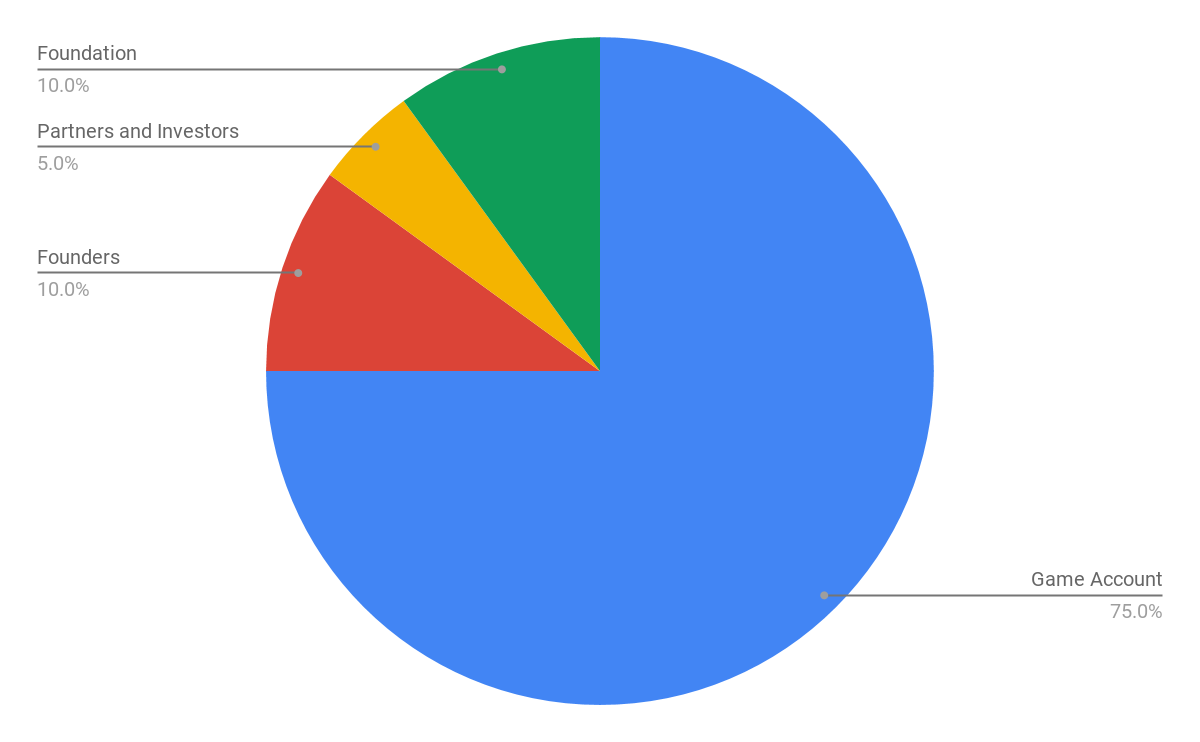
\includegraphics[width=6.27in,height=3.88in]{./media/image26.png}
		\caption{Chart showing the allocation of GOLD.}
		\label{fig:Chart_showing_the_allocation_of_GOLD}
	\end{FlushLeft}\end{figure}


%%%%%%%%%%%%%%%%%%%% Figure/Image No: 15 Ends here %%%%%%%%%%%%%%%%%%%%


\textbf{The Treasury}\par

As Dragonereum will not have any kind of initial coin offerings or a sale, the majority (75$\%$ ) of tokens will be allocated to the Treasury (shown in blue in Figure \ref{fig:Chart_showing_the_allocation_of_GOLD}).\par

Cybernomics of the game is based on the willingness of players to evolve better dragons: as dragons with higher DS are likely to earn more Gold.\par

The more dragons are battling, the more expensive it becomes to earn Gold from the Treasury (please see \ref{Early adopter advantage}). The Treasury is guaranteed to be replenished with players' Gold payments for incubation through embedded genetics mechanism. This basic feedback loop stimulates GOLD internal liquidity.\par

Cybernomics also determines the population specifications: dragons are very cheap to generate at the Genesis, thus stimulating aggressive population growth in order to become dominant species in the Ethereum universe.\par

During early stages of the game there is an incentive for a faster population growth, as available  supply of Gold inflates faster than its deflation occurs (originating from the environmental costs of incubation).\par

Similar to the real world, evergrowing population is strictly limited by available resources. Once environmental resources become scarcer deflation starts dominating over inflation thus securing the store of value for players who have managed to earn more Gold.\par

\textbf{Founders}\par

Once the smart contract is deployed, appointed team members will receive a total of 10$\%$ of tokens in their possession (shown in red in Figure \ref{fig:Chart_showing_the_allocation_of_GOLD}) in accordance with individual contribution to the project in a form of funding, development, design, drawings, etc conducted before Genesis.\par

\textbf{Nonsense Games}\par

Nonsense Games will receive another 5$\%$ (shown in yellow in Figure \ref{fig:Chart_showing_the_allocation_of_GOLD}) as a reward for the contribution of the team to the project before Genesis. The multisig address of Nonsense Games is 0x10208fb4ef202bdc49803995b0a8ca185383bba4.\par

\textbf{The Foundation}\par

The remaining 10$\%$  will be used for the Dragonereum ecosystem development and community building (shown in green in Figure \ref{fig:Chart_showing_the_allocation_of_GOLD}). This may include (but not necessarily):\par

\begin{itemize}
	\item New team members and advisors\par

	\item Liquidity pool (eg. Bancor)\par

	\item Airdrop\par

	\item Security audits\par

	\item Bounty campaigns (eg. Gitcoin).
\end{itemize}\par

Overall purpose of the Foundation is to stimulate liquidity of Gold by increasing its consumption by basic protocol contracts and auxiliary contracts which return Gold to the Treasury. Examples of such contracts can be name registries, trading protocols, bridges to other networks, etc.\par

The multisig address of the Foundation is 0x5ff8957ef7e964e8072815211c9fc3e7f820f1d4.\par

 %%%%%%%%%%%%  Starting New Page here %%%%%%%%%%%%%%

\newpage

\vspace{\baselineskip}\section{Conclusion}
%\addcontentsline{toc}{section}{Conclusion}
In this document we described a blockchain cryptocollectible PvP game built on the Ethereum network which emphasizes the advantages of the blockchain solutions for future blockchain gaming, gambling and collectible markets.  \par

The technological and socioeconomic solutions for creation of a sustainable game ecosystem were examined and discussed.\par

A thorough description of the game’s details and rules was provided. Further, we showed that Dragonereum is made with the current constraints of the blockchain technology in mind.\par

A description of the in-game cryptocurrency, Gold, was given and it was shown that its value will grow.  \par

In addition, we presented a large variety of possible future integrations of the game.\par

\vspace{\baselineskip}

 

\newpage
\printbibliography

\newpage
\section*{Appendix}
\addcontentsline{toc}{section}{Appendix}
 % \appendix  \par


%\vspace{\baselineskip}
  \begin{Large}
  {Regular Battles}%&\label{Regular Battles}  \par
  \end{Large}


\vspace{\baselineskip}
Below is the code describing the execution of the regular battles.\par

\begin{footnotesize}
\begin{verbatim}
   function _resetBlocking(Dragon dragon) internal pure returns (Dragon) {
        dragon.blocking = false;
        dragon.specialBlocking = false;
        return dragon;
    }

    function _attack(uint8 turnId, bool isMelee, Dragon attacker, Dragon opponent, uint8 
_random) internal pure returns (Dragon, Dragon) {
        uint8 _turnModificator = 10; // multiplied by 10
        if (turnId > 30) {
            // _turnModificator = uint8(1 * 10 + uint16((turnId - 30) * 10 * 5) / 40);
            // hack "stack too deep" error
            uint256 _modif = uint256(turnId).sub(30);
            _modif = _modif.mul(50);
            _modif = _modif.div(40);
            _modif = _modif.add(10);
            _turnModificator = _modif.toUint8();
        }

        bool isSpecial = _random < _multiplyByFloatNumber(attacker.specialAttackChance, 
_turnModificator);
        uint32 damage = _multiplyByFloatNumber(attacker.attack, _turnModificator);
        if (isSpecial && attacker.mana >= attacker.specialAttackCost) {
            attacker.mana = attacker.mana.sub(attacker.specialAttackCost);
            damage = _multiplyByFloatNumber(damage, attacker.specialAttackFactor);
        }
        if (!isMelee) {
            damage = _multiplyByFloatNumber(damage, DISTANCE_ATTACK_WEAK__);
        }
        uint32 defense = opponent.defense;
        if (opponent.blocking) {
            defense = _multiplyByFloatNumber(defense, DEFENSE_SUCCESS_MULTIPLY__);
            if (opponent.specialBlocking) {
                defense = _multiplyByFloatNumber(defense, opponent.specialDefenseFactor);
            }
        } else {
            defense = _multiplyByFloatNumber(defense, DEFENSE_FAIL_MULTIPLY__);
        }
        if (damage > defense) {
            opponent.health = _safeSub(opponent.health, damage.sub(defense));
        } else if (isMelee) {
            attacker.health = _safeSub(attacker.health, defense.sub(damage));
        }

        return (attacker, opponent);
    }

    function _defense(Dragon attacker, uint256 initialSeed, uint256 currentSeed) internal 
pure returns (Dragon, uint256) {
        uint8 specialRandom;
        (specialRandom, currentSeed) = _getRandomNumber(initialSeed, currentSeed);
        bool isSpecial = specialRandom < attacker.specialDefenseChance;
        if (isSpecial && attacker.mana >= attacker.specialDefenseCost) {
            attacker.mana = attacker.mana.sub(attacker.specialDefenseCost);
            attacker.specialBlocking = true;
        }
        attacker.blocking = true;
        return (attacker, currentSeed);
    }

    /* solium-disable-next-line security/no-assign-params */
    function _turn(
        uint8 turnId,
        uint256 initialSeed,
        uint256 currentSeed,
        uint32 distance,
        Dragon currentDragon,
        Dragon currentEnemy
    ) internal view returns (
        Dragon winner,
        Dragon looser
    ) {
        uint8 rand;

        (rand, currentSeed) = _getRandomNumber(initialSeed, currentSeed);
        bool isAttack = rand < currentDragon.attackChance;

        if (isAttack) {
            (rand, currentSeed) = _getRandomNumber(initialSeed, currentSeed);
            bool isMelee = rand < currentDragon.meleeChance;

            if (isMelee && distance > MAX_MELEE_ATTACK_DISTANCE) {
                distance = _safeSub(distance, currentDragon.speed);
            } else if (!isMelee && distance < MIN_RANGE_ATTACK_DISTANCE) {
                distance = distance.add(_multiplyByFloatNumber(currentDragon.speed, FALLBACK_SPEED_FACTOR__));
            } else {
                (rand, currentSeed) = _getRandomNumber(initialSeed, currentSeed);
                (currentDragon, currentEnemy) = _attack(turnId, isMelee, currentDragon, 
currentEnemy, rand);
            }
        } else {
            (currentDragon, currentSeed) = _defense(currentDragon, initialSeed, currentSeed);
        }

        currentEnemy = _resetBlocking(currentEnemy);
        if (currentDragon.health == 0) {
            return (currentEnemy, currentDragon);
        } else if (currentEnemy.health == 0) {
            return (currentDragon, currentEnemy);
        } else if (turnId < MAX_TURNS) {
            return _turn(turnId.add(1), initialSeed, currentSeed, distance, currentEnemy, 
currentDragon);
        } else {
            uint32 _dragonMaxHealth;
            uint32 _enemyMaxHealth;
            (_dragonMaxHealth, ) = getter.getDragonMaxHealthAndMana(currentDragon.id);
            (_enemyMaxHealth, ) = getter.getDragonMaxHealthAndMana(currentEnemy.id);
            if (_calcPercentage(currentDragon.health, _dragonMaxHealth) >= 
_calcPercentage(currentEnemy.health, _enemyMaxHealth)) {
                return (currentDragon, currentEnemy);
            } else {
                return (currentEnemy, currentDragon);
            }
        }
    }

\end{verbatim}
\end{footnotesize}


\vspace{\baselineskip}

\vspace{\baselineskip}
%  \section{Gladiator Battles}\label{Gladiator Battles}  \par


%\vspace{\baselineskip}

%\printbibliography
\end{document}